\documentclass[12pt]{report}
\usepackage[portuguese]{babel}
\usepackage[utf8]{inputenc}
%\usepackage[dvips]{graphicx}
\usepackage{graphicx}
\usepackage{enumitem}
\usepackage[normalem]{ulem}
\usepackage{latexsym}
\usepackage{amsmath}
\usepackage{float}
\usepackage{units} % Para frações bonitas
\usepackage{verbatim} % Para que o bloco {comment} funcione
\usepackage[pdfborder={0 0 0}]{hyperref}
\usepackage{wrapfig} % Para o qrcode do editorial
\usepackage[labelformat=empty]{caption} % Para tirar o "Figure:" da caption do QRCode

%\usepackage{showframe} %Para mostrar o frame do arquivo

\newcounter{qcounter}

\setlength{\parindent}{0pt}
\setlength{\parskip}{3ex plus 0.5ex minus 0.5ex}

\addtolength{\voffset}{-2.8cm}
\addtolength{\textheight}{5.5cm}
\addtolength{\hoffset}{-2.3cm}
\addtolength{\textwidth}{4.5cm}
\setlength{\topmargin}{0cm}

%FIXME GAMBIARRA
%\setlength{\evensidemargin}{55pt}

\pagestyle{plain}

% =============== Seção de definições de macros ========================

% Delimita uma seção:
\newenvironment{secao}[1] {
    \framebox[\textwidth] {
        \rule[-1.2ex]{5ex}{5.5ex}
        {\Large\sf #1}
        \hspace{\stretch{1}}
    }
    \phantomsection %Faz o link do pdf funcionar direito
	\addcontentsline{toc}{chapter}{#1}
    \nopagebreak[4]
}{}

%FIXME Isso pode ser resolvido de um jeito melhor, fazendo uma seção (editorial e mandamentos)
% não entrarem no índice usando uma tag, e não outro tipo de environment.
% Veja a primeira linha de editorial.tex para entender melhor.
% Delimita o editorial (que não entra no Índice):
\newenvironment{editorial}[1] {
    \framebox[\textwidth] {
        \rule[-1.2ex]{5ex}{5.5ex}
        {\Large\sf #1}
        \hspace{\stretch{1}}
    }
    \phantomsection %Faz o link do pdf funcionar direito
    %\addcontentsline{toc}{chapter}{#1}
    \nopagebreak[4]
}{
\thispagestyle{empty}
\pagebreak
}


% Delimita uma subseção
\newenvironment{subsecao}[1] {
    \rule[0ex]{2.5ex}{2.5ex}
    {\Large\sf #1}
    \phantomsection %Faz o link do pdf funcionar direito
	\addcontentsline{toc}{section}{#1}
    \nopagebreak[4]
}{}

% Delimita uma subsubseção
\newenvironment{subsubsecao}[1] {
    \rule[0ex]{1ex}{1.5ex}
    {\large\sf #1}
    \phantomsection %Faz o link do pdf funcionar direito
% Próxima linha é responsável por subsubseções não aparecerem no índice!
	%\addcontentsline{toc}{subsection}{#1}
    \nopagebreak[4]
}{}

% Coloca uma figura grande (sem ser quadrinhos)
\newcommand{\figuragrande}[1] {
    \begin{figure}[!htbp]
      \begin{center}
        \includegraphics[width=\textwidth]{img/#1.pdf}
      \end{center}
    \end{figure}
}

% Coloca uma figura menor (sem ser quadrinhos)
\newcommand{\figurapequenainline}[1] {
  \begin{wrapfigure}{r}{0.25\textwidth}
    \vspace{-25pt}
    \begin{center}
      \includegraphics[width=0.25\textwidth]{img/#1.pdf}
    \end{center}
    \vspace{-25pt}
  \end{wrapfigure}
}

% Coloca uma figura menor (sem ser quadrinhos) apertada verticalmente
\newcommand{\figurapequenainlineflexivel}[2] {
  \begin{wrapfigure}{r}{0.25\textwidth}
    \vspace{-#2}
    \begin{center}
      \includegraphics[width=0.25\textwidth]{img/#1.pdf}
    \end{center}
    \vspace{-#2}
  \end{wrapfigure}
}

% Coloca uma figura menor (sem ser quadrinhos) apertada verticalmente
\newcommand{\figurapequenainlineapertada}[1] {
  \begin{wrapfigure}{r}{0.25\textwidth}
    \vspace{-40pt}
    \begin{center}
      \includegraphics[width=0.25\textwidth]{img/#1.pdf}
    \end{center}
    \vspace{-40pt}
  \end{wrapfigure}
}

% Coloca quadrinhos
\newcommand{\quadrinhos}[1] {
    \figuragrande{quad#1}
}

% Coloca um mapa
\newcommand{\mapa}[1] {
	\begin{figure}[H]
		\centering
		\includegraphics[height=\textwidth, angle=90]{img/#1}
	\end{figure}
}

%FIXME GAMBIARRA
% Coloca um mapa do IME virando ele do jeito certo
\newcommand{\mapaime}[1] {
    \begin{figure}[H]
        \centering
        \includegraphics[width=\textwidth, angle=180]{img/#1.pdf}
    \end{figure}
}



% ============================ Documento ===============================
\begin{document}

% Capa -------------------------------------------------------------------------
\begin{figure}[p]
  %\begin{center}
    %\hspace{1.7cm}
    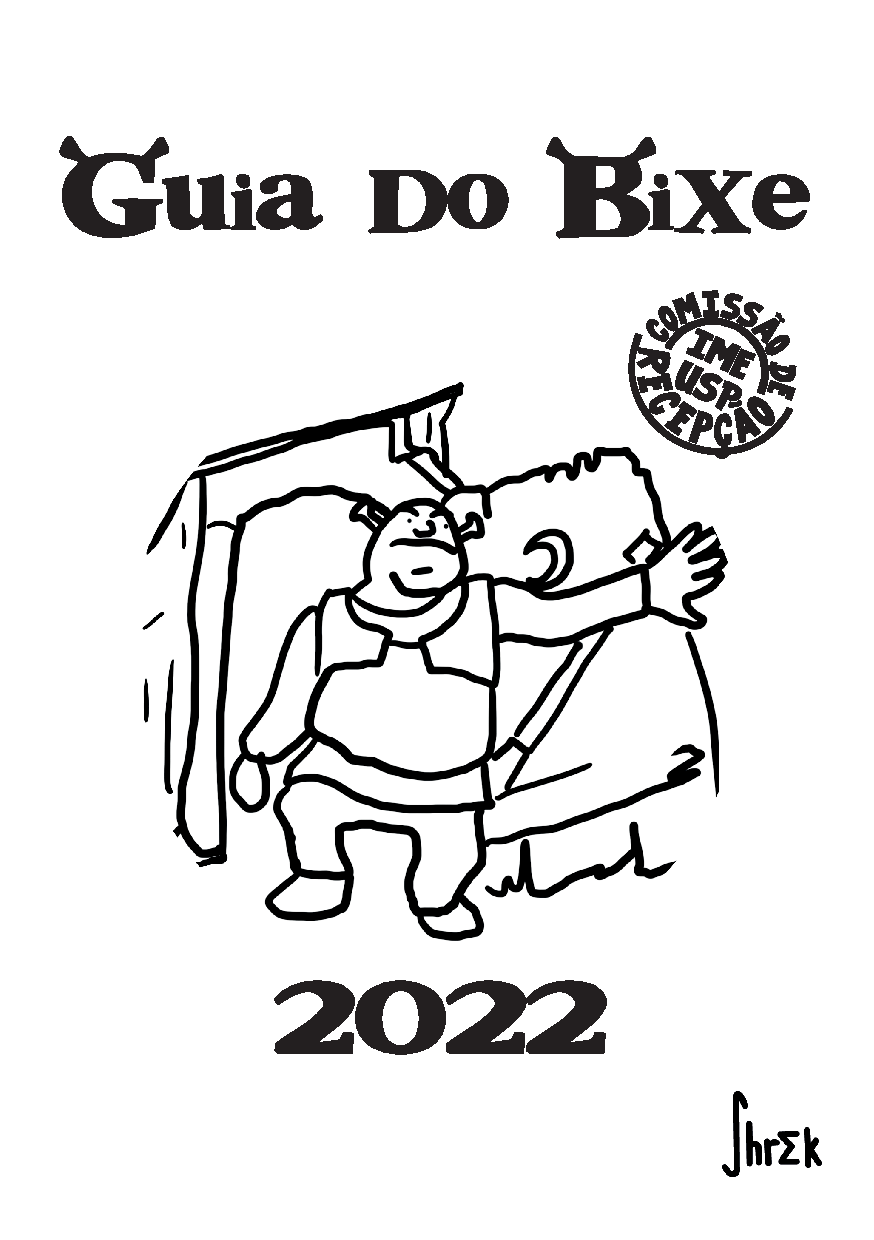
\includegraphics[height=1\textheight]{img/capa_2022.pdf} %REFTIME
  %\end{center}
\end{figure}
\thispagestyle{empty} % Some com aquele número 1 feio na capa.
\clearpage
\newpage

% Começa a numeração aqui para que o LaTeX entenda qual
% página é ímpar e qual é par antes do índice.
\pagenumbering{arabic}

% Pré-Índice -------------------------------------------------------------------
\begin{editorial}{Editorial}

Bixes, foi difícil chegar até aqui. Vocês
estão meio ou completamente perdidos. Temos apenas uma sugestão: aproveitem esta
etapa! Façam da sua estadia na USP a melhor época das suas vidas! Vocês verão
que a USP tem muitas e muitas coisas a oferecer! Não se preocupem apenas em
estudar e passar de ano, como vocês fizeram durante sua vida inteira; aproveitem
TUDO! Vocês podem não acreditar nisso agora, mas saibam que viverão momentos
inesquecíveis aqui no IME: alguns fantásticos, outros deploráveis.

Este guia foi feito para que vocês (bixes que não gostam de ler, apenas olhem as figuras)
possam aprender um pouquinho do que é a USP,
o IME e a vida universitária que se inicia agora. 
Gostaríamos que guardassem este guia com muito carinho para que, futuramente, possam consultá-lo
quando surgir alguma dúvida do que fazer em determinada situação!

O guia foi escrito numa forma
descontraída e fácil para que vocês consigam entender; mesmo assim, se aparecer
alguma dúvida, vocês podem se dirigir a qualquer veterane, e sua dúvida será
sanada (e, quem sabe, talvez você também comece uma nova amizade).

Além disso, ao invés de usarmos as palavras ``bixos'' ou ``bixetes'', vamos nos referir
a vocês como ``bixes'', pois estamos dirigindo palavra a todas as identidades de 
gênero! Por motivos de vocabulário e acessibilidade, usamos a linguagem neutra 
apenas em ``bixes'' e ``veteranes''.

%Empurra pro fim da página (altura)
%\vspace{\stretch{1}}

%Linha divisória
\rule{\textwidth}{0.5ex}\rule{2ex}{0.5ex}

%REFTIME
{\large\bf Guia de Bixe 2024} \\
Uma publicação da Comissão de Recepção


\begin{wrapfigure}{R}{0.25\textwidth}

% Link para "https://ime.usp.br/~kazuo/guia"
% Esse link contém um contador de acessos que redireciona para o guia correto
% Em 2020: https://ime.usp.br/~kazuo/guiadobixo.pdf
  \begin{center}
    
\includegraphics[width=0.22\textwidth]{img/qrcode_guia2023.pdf}
  \end{center}
  \vspace{-20pt}
  \caption{Baixe aqui o Guia em formato digital!}
  \vspace{80pt}
\end{wrapfigure} 

Muitas pessoas dedicaram seu tempo (e suas férias) para que esse Guia ficasse
pronto: desde o Donald Knuth em 1978, na criação do \TeX\makebox{}, até o
pessoal da Comissão na correria de ontem à noite. Esperamos que vocês gostem do Guia
e adotem-no como livro de cabeceira. Por fim, nos avisem de qualquer informação
incorreta ou desatualizada, afinal vocês também são responsáveis por tudo que o
IME oferece a partir de agora.

Lembrem-se: este é o primeiro e último ano de vocês como bixes. Aproveitem!
%\vspace{2em}

%REFTIME (Capa muda todo ano)
%Capa de 2022: ???
%Capa de 2021: ???
%Capa de 2020: ???
%Capa de 2019: ???
%Capa de 2018: ???
%Capa de 2017: ???
%Capa de 2016: public domain
%Capa de 2015:
%{\bf Imagem da Capa:} Viktoria Ridzel -- \href{www.viria13.deviantart.com}{viria13.deviantart.com}

Este trabalho está licenciado sob a Licença Attribution-ShareAlike 4.0 da
Creative Commons. Para ver uma cópia desta licença, visite
\url{https://creativecommons.org/licenses/by-sa/4.0/deed.pt_BR} ou envie
uma carta para Creative Commons, 444 Castro Street, Suite 900, Mountain View,
California, 94041, USA.
\\
\begin{figure}[H]
    \centering
    \includegraphics{img/cc/by-sa.png}
\end{figure}

\end{editorial}


% Carta Aos Ingressantes -------------------------------------------------------
\begin{editorial}{Carta Aos Ingressantes}

Agora que vocês entraram na USP, bixes, adquiriram novas
responsabilidades. Vocês são responsáveis pelas suas próprias vidas, isto é, 
ninguém irá se preocupar com seus problemas acadêmicos (matrículas, notas erradas,
dificuldades com algumas matérias, rixas com professores, etc.) se vocês não se
preocuparem. Existem pessoas que podem lhes ajudar, mas só o farão se vocês
forem procurá-las. Caso contrário, as únicas pessoas prejudicadas serão vocês.

A faculdade não é o Paraíso (essa estação fica perto da Avenida Paulista), mas pode
melhorar a cada dia. Nós, alunes, também devemos contribuir para essa melhora.
Vocês são o \textbf{futuro da Universidade}. Portanto, participem, reclamem, busquem seus
direitos, ajudem e, principalmente, não tenham medo de cara feia, pois isso é o
que não vai faltar.

Lembrem-se que vocês não são mais crianças e já sabem o que querem sem que
outros precisem decidir por vocês; então procurem o que lhes interessa: iniciação
científica, estágios, monitorias, matérias que não são obrigatórias, mas que
vocês gostariam de fazer (mesmo que não tenham nada a ver com seu curso ou que não
sejam no IME), participação no CAMat ou na Atlética, esportes no CEPE, artigos no
jornal, etc., etc., etc.

Não é só porque vocês podem, que vocês devem fazer tudo sozinhes, portanto lembrem que
as amizades vão ser \textbf{muito importantes} para vocês e para o bom andamento do seu
curso. Procurem combinar atividades fora da faculdade, diferentes do cotidiano,
porque isso ajuda a amenizar o estresse que o dia a dia na faculdade pode
trazer.

Além de tudo, vocês não podem se esquecer de uma parte importante de suas vidas
na universidade, que é \textbf{estudar}. Tentem não deixar para estudar na véspera da
prova, porque a probabilidade de vocês não irem bem é altíssima (exceto se vocês
tiverem uma sala do tempo em casa, que nem a do Dragon Ball). A mesma coisa se
aplica aos EPs, ainda mais porque, quanto mais próximo da data de entrega, mais
erros vão aparecer e, na maioria dos casos, os EPs não são aceitos depois da
data limite de entrega e, caso sejam aceitos, não valerão a mesma nota.

Além disso, como em todo lugar, existem aquelas pessoas ranzinzas e
pentelhas que acham super bacana acabar com a graça de todo mundo,
criticar o IME e aumentar a sua baixa autoestima dizendo que os cursos
são impossíveis e que vocês não vão se formar nunca, mas não acreditem
nelas! Vocês entraram aqui com um propósito. Sigam-no!  

\textbf{Obs.:} não se assustem com palavras e siglas que vocês não entenderam ou 
não entenderem! Continuem lendo, porque tudo será explicado em detalhes, 
mastigado, tim-tim por tim-tim. Saibam que vai faltar um monte de siglas...  
Aprendam-nas seletiva e rapidamente. Destaques para: USP, IME, MAC,
MAT, MAE, MAP, BCC, BM, BMA, LIC, BMAC, BE, CEPE, CEAGESP, CTA, RD, CAMat,
AAAMat, SSG, P1, P2, P3, P4, P5, Pn, PQP, CEC, CNPq (=\$), FAPESP
(=\$\$\$), CG, DP, REC, SUB (esta última, ou talvez as duas ou três últimas,
vocês vão conhecer bem melhor, mais cedo ou mais tarde).

\end{editorial}


% Os Dez Mandamentos -----------------------------------------------------------
\begin{editorial}{Os Dez Mandamentos}

\begin{enumerate}
  \item Os veteranes têm sempre razão, exceto quando os bixes têm;
  \item Na hipótese de o bixe ter razão, entra imediatamente em vigor
        o primeiro mandamento;
  \item Em qualquer evento social, as despesas correm sempre por conta dos
        bixes, menos o que os veteranes consomem;
  \item Os bixes têm o direito de permanecerem calados (exceto quando
        interpelados por veteranes ou quando quiserem falar). Tudo o que eles
        disserem pode ser usado contra eles, \textit{c’est la vie};
  \item Os bixes devem se apresentar imediatamente em caso de convocação por
        veteranes, a não ser que estejam fazendo algo melhor da vida. Os bixes
        que não se apresentarem se arrependerão amargamente por perderem
        conselhos valiosos; %não queremos ameaçar ninguém :)
  \item Não são garantidos no IME os direitos constitucionais dos bixes à vida
        social, liberdade de sono e igualdade de notas;
  \item Os bixes devem estar prontos para assumirem as seguintes funções para
        veteranes: completar mesa de jogo, companhia de bandejão, completar
        time(s) etc., mas somente quando tiverem vontade;
  \item Os bixes devem amar e respeitar seus veteranes, a vida, as plantas,
        todo mundo e acima de qualquer coisa, Goku;
  \item Para os casos não abrangidos por estas regras, a decisão final correrá
        por conta dos veteranes, com exceção do que não lhes diz respeito;
  \item Todos os bixes estão despreparados, exceto os que leram isto.
\end{enumerate}

Como bixes, vocês têm todo o direito de reclamar dos mandamentos! 
Qualquer reclamação deverá ser protocolada em três vias datadas, assinadas e
autenticadas, com firma reconhecida em cartório, e assim encaminhadas à
Comissão de Recepção 2024 %REFTIME
via mala direta e serão imediatamente incineradas. Alguns veteranes sugeriram
que incinerássemos os reclamantes também. Ao invés disso, cogitamos incinerar
tais veteranes. A medida passou por estudo e, devido aos custos operacionais e
ao lixo tóxico que seria produzido, foi rejeitada.

OU vocês podem conversar diretamente com um veterane da Comissão :)

\end{editorial}


% Os Sete Pecados --------------------------------------------------------------
%PANDEMIA - esta seção foi totalmente refeita! Quando as aulas online acabarem, fazer
          % a revisão anual tendo como base o guia de 2020 (e talvez algumas coisas
          % do online, se elas se mantiverem).
\begin{editorial}{Os 7 pecados cometidos por bixes}

\begin{itemize}
  \item Dizer que cursa ``matemática'' (bixes, vocês cursam
        lic/pura/aplicada/bcc/estat/bmac...);
  \item Procurar pelo Jupiter no Google e encontrar uma imagem do planeta;
  \item Esquecer o dia da prova;
  \item Esquecer de fazer a matrícula;
  \item Atrasar a devolução de livros na biblioteca;
  \item Entregar a versão errada do EP, ou pior, entregar em \texttt{*.doc};
  \item Não saber que o professor cancelou a aula;
  \item Frequentar a turma errada da matéria;
  \item Se matricular em uma matéria em um campus do interior sem querer;
        %(agora podem fazer isso sem medo!);
  \item Esquecer do prazo de trancamento;
  %\item Entrar na aula on-line com a câmera ligada enquanto ainda nem saiu da cama;
  %\item Largar a aula síncrona aberta, ir fazer outra coisa e esquecer de sair antes da aula acabar;
  %\item Esquecer o microfone aberto enquanto fala com outras pessoas;
  \item Não saber quem é o Goku.
%\end{itemize}
%Os pecados a seguir são os que (ainda) não fazem muito sentido para vocês que
%estão entrando virtualmente no IME, mas vamos manter todos aqui, porque
%achamos que é bom vocês já saberem sobre eles (se não entenderem,
%tudo bem! Recomendamos perguntar para veteranes):

%\begin{itemize}
  \item Pegar o circular errado;
  \item Ir bandejar sem crédito no cartão USP;
  \item Jogar o talher do bandejão no lixo;
  \item Confundir o bilhete único com o BUSP e pagar o circular;
  \item Comprar na lanchonete;
  \item \sout{Não ter moeda para a máquina de café}\footnote{Quando escrevemos
    esse pecado, era sobre a nossa querida Jennifer (R.I.P.), que aceitava
    moedas. Conheça-a em \url{fb.com/jennifer.maccafe}} Pagar um café da
    máquina e só depois descobrir que acabaram os copos (ou açúcar, ou café,
    ou qualquer outra coisa);
  \item Achar que o P3 é perto;
  \item Ir para a aula só para assinar a lista, e o professor não passar lista;
  \item Desperdiçar quota na impressora sem papel;
  \item Deixar o computador logado na Linux ou no CEC e ser trollado;
  \item Acender a luz da vivência antes das 8h da manhã;
  \item Atrapalhar a aula gritando alto demais no truco;
  %\item Se matricular em uma matéria em um campus do interior sem querer, quando
  %      voltarmos a ter aula presencial;
\end{itemize}
e, por último, mas não menos importante,
\begin{itemize}
  \item Não saber contar quantos pecados tem na lista de 7 pecados.
\end{itemize}

\end{editorial}



%Renomeando o índice------------------------------------------------------------
\renewcommand{\contentsname}{\center Esse guia contém...}

% Coloca o índice --------------------------------------------------------------
\tableofcontents
% Remove números de página do índice
\thispagestyle{empty}
\addtocontents{toc}{\protect\thispagestyle{empty}}
\addtocontents{toc}{\protect\pagestyle{empty}}
\newpage
\thispagestyle{empty}
\cleardoublepage

% Começa a numeração aqui
\pagenumbering{arabic}


% Comissão de Trote e o Kit-bixe -----------------------------------------------
\begin{secao}{Comissão de Recepção e \textit{Kit}-bixe}

A Comissão de Recepção aos Calouros, também conhecida apenas como Comissão de
Recepção, é responsável por auxiliar os ingressantes em seus primeiros momentos
IMEanos. Sabemos que não é um momento fácil. Vocês estão entrando em uma nova fase
de suas vidas, em um lugar estranho, com pessoas estranhas (em todos os sentidos),
e nosso objetivo é fazer com que vocês se sintam bem-vindos e se integrem
($\int$) com seus coleguinhas e seus veteranes!

A Comissão de Recepção organiza a super Semana de Recepção, cheia de atividades
legais! (Vejam a programação em: \url{https://recepcao.ime.usp.br/}!).
Somos nós também que organizamos o magnífico encontro dos bixes: AnIME-se.
Atente-se à página da Comissão no Facebook para quando a data for divulgada.

A Comissão de Recepção é formada pelos mais animados e divertidos veteranes. Como
dissemos, eles organizam a Semana de Recepção, ajudam bixes perdidos, mantêm um clima
alegre durante a recepção, fazem isso e aquilo...
Vocês devem estar pensando ``Puxa! Como nós, bixes, podemos retribuir
tamanha dedicação?'' É simples, bixes: {\bf\em comprem o \textit{kit}-bixe}!!!

O \textit{kit}-bixe, como vocês devem saber, é um conjunto de coisas
importantíssimas para vocês, ingressantes perdidos! Ele contém dois tipos de
itens:
\begin{itemize}
\item itens úteis;
\item itens essenciais.
\end{itemize} %REFTIME (Isso muda todo ano)
Dentre eles, temos uma camiseta com uma linda estampa do tema do ano de vocês,
que serve para que nós os identifiquemos como bixes e para que as pessoas
achem que vocês são inteligentes; um lindo estojo com o símbolo do IME e vários materiais
para vocês usarem nas aulas e mostrarem aos seus amigos; uma caneca e um talabarte MARAVILHOSOS
(também personalizados) para vocês economizarem muitos copos no bandejão; um
chaveiro personalizado muito maneiro que também serve para abrir garrafas;
dois adesivos, um para vocês colarem no carro que vão ganhar de presente, e outro
para os papais (quando vocês virem o adesivo vocês vão entender); e um caderno super
lindo e sem pauta para vocês desenharem seus gráficos das aulas de Cálculo. Tudo
isso preparado com muito carinho e especialmente para vocês pela Comissão de Recepção,
além de estarem contidos em uma mochila sport do IME-USP, afinal, não dá pra
carregar tudo isso na mão, né?

Além dessa maravilha de \textit{kit}-bixe, vocês ainda podem adicionar à parte bottons
exclusivos e personalizados com o símbolo do IME-USP e com o tema da recepção.

Adquiram o maravilhoso \textit{kit}-bixe do IME-USP! Fiquem atentos às redes sociais da
Comissão de Recepção para saberem quais os períodos em que as vendas estarão abertas.
O kit estará à venda na Semana de Recepção e inclusive na semana subsequente em
\url{https://cheersshop.com.br/recepcaoimeusp} mas somente enquanto
durarem os estoques. (Não vão chorar depois, hein?)

Para terminar, além de tudo isso, a Comissão de Recepção é que faz esse maravilhoso guia que
vocês estão lendo agora (ou estão só olhando as figuras, vai
saber...). Esperamos que vocês gostem do nosso trabalho! Qualquer coisa, nos
procurem! Entrem na nossa página no Facebook (\url{fb.com/recepcaoimeusp}) ou no nosso
Instagram (\url{instagram.com/recepcaoimeusp}) contando
o que vocês sentiram ao ler o guia, o que fizeram de errado com vocês na
recepção (com o nome do veterane na denúncia), o que vocês acharam da Semana
de Recepção e se vocês se sentiram bem-vindos . Estaremos sempre prontos a ajudá-los!
\end{secao}

\quadrinhos{1}

% O CAMat ----------------------------------------------------------------------
\begin{secao}{O CAMat}

CAMat é a sigla para Centro Acadêmico da Matemática, Estatística e Computação 
"Elza Furtado Gomide". Bom, o que faz um centro acadêmico? 
O centro acadêmico é a entidade representativa dos estudantes (conhecido 
também como entidade de base), ele serve para organizar o movimento estudantil
dentro do Instituto, lutando por melhorias internas no IME, e também
participando de assuntos da política da USP e de fora dela.

No caso do CAMat, representamos todos aqueles matriculados na graduação e pós-graduação do IME-USP.

O administrativo da entidade fica no interior da Vivência (sala 18 do bloco B), lá você 
poderá encontrar uma vendinha de guloseimas e bebidas para matar a larica e sede nossa de
cada dia. Como a Vivência,  o acesso é livre e aberto a todos! Além dos
comes e bebes, também emprestamos - mediante a apresentação do cartão USP -
calculadoras científicas, baralhos e outros jogos de carta! Na Vivência em si, temos sofás
para vocês passarem um tempo, tirar um cochilo, jogar sinuca ou Smash, e
também armários para alugar. Enfim, a Vivência + CAMat são o espaço de convivência 
dos estudantes, com a manutenção e organização de responsabilidade do centro acadêmico 
- o que não exclui a necessidade de qualquer um que frequente o espaço também se 
empenhar na conservação da limpeza e ordem na Vivência.

Importante reforçar que a atuação do CAMat não se basta à salinha ou à Vivência. 
O centro acadêmico é responsável por diversos projetos - a exemplo, CinIME e Aulões 
-, e também promove eventos para maior integração entre os estudantes e o espaço do 
instituto e da universidade. Aliás, caso você tenha propostas de eventos ou projetos, 
fale conosco, dado que sendo o meio dos estudantes agirem e se organizarem na luta pela 
universidade popular, estamos sempre abertos ao debate de ideias e a fomentação de discussões 
construtivas. O diálogo com os estudantes é essencial para que a gestão seja ativa e presente no IME!

Veja a seguir um pouco sobre os projetos do CAMat:


\begin{subsecao}{Banco de Provas}

O CAMat, conjuntamente com os estudantes, organizam um Banco de Provas
\href{https://camat.ime.usp.br/apoio/} com VÁAAARIAS provas dos anos 
anteriores feitas pelos maravilhosos veteranes.

Não se esqueça de contribuir com sua prova ao final do semestre, não
deixe o Banco de Provas morrer! 

\end{subsecao}

%\begin{subsecao}{Aulões do CAMat e Oficina de Demonstrações}

%Os aulões são atividades promovidas pelo CAMat para ajudar os bixes com as
%disciplinas do primeiro ano do curso. Muitas vezes algum veterane que tem mais
%experiência em certa disciplina se oferece para dar uma aula tirando as dúvidas
%mais comuns e tentando passar um ponto de vista diferente para complementar e facilitar
%as aulas. As vezes os professores do IME podem ajudar também, como é o caso da Oficina 
%de Demonstrações que foi ministrada por uma professora para ajudar os bixes a entenderem 
%melhor como se faz uma prova matemática rigorosa, e até se tornou uma bolsa PUB para que alunos
%possam estudar mais sobre o uso dessa ferramenta pedagógica. 
%Participem dos aulões e usem esse espaço para tirar suas dúvidas e complementar as aulas!

%\end{subsecao}

\begin{subsecao}{CinIME}

Com a proposta de pautar de maneira mais crítica quais, como e onde consumimos 
entretenimento audiovisual, o CAMat organiza as atividades de cinema no IME 
como parte de um momento de reflexão, mas também de lazer. Afinal, cinema e 
pipoquinha são legais e todo mundo gosta! Toda sexta-feira são exibidos filmes 
diferentes com pipoca e refrigerante de graça, e as sessões são abertas a todos 
os alunos, funcionários e docentes. O CinIME também tem um espaço exclusivo nesse
guia para que vocês possam saber mais detalhes.

\end{subsecao}

\begin{subsecao}{Chá Mate e BoletIME}

Chá Mate é o encontro mensal que o CAMat organiza para os estudantes debaterem temas
ligados à política e à vida universitária. Desde a criação do Chá Mate, já discutiu-se
desde a falta de água no CRUSP até a elitização do acesso ao futebol (esse tema com parceria
da Atlética). Sempre buscamos trazer um material de apoio, que pode ser um texto, podcast, matéria
de jornal ou qualquer outra coisa que seja útil para abordar o assunto. 
Além disso, a organização do Chá Mate edita o BoletIME, uma espécie de jornal dos alunos do IME em
que publicamos entrevistas, notícias sobre a USP, editoriais políticos, repasses dos Representantes
Discentes e novidades do Centro Acadêmico. Toda a comunidade estudantil IMEana é bem vinda a construir
o BoletIME conosco: existe um forms para enviar textos, e você pode falar sobre qualquer assunto da sua
experiência universitária. Você pode conferir a última edição do BoletIME em formato 
digital no site do CAMat, e em formato impresso na salinha do CAMat na vivência.

\end{subsecao}


\begin{subsecao}{An(IME)\texorpdfstring{$^2$}{²}}

An(IME)$^2$ é o evento de animes e mangás do IME, organizado pelo CAMat. Entre as atrações,
contamos com PokéBingo, Just Dance, Karaokê, concurso de Cosplay e de Cospobre e uma sessão 
especial do CinIME.
Também é quando você pode comprar o já tradicional Kit Otaku, que normalmente vem com uma
caneca, uma camiseta e um caderno temáticos de anime, além dos bottons exclusivos do evento.
É um dia para o IMEano liberar o seu lado otaku e correr solto pelo Instituto depois de
encher a cara de Mupy!

\end{subsecao}

\begin{subsecao}{Campeonato de Sinuca}

Se você gosta de jogar sinuca, cola na Vivência que a mesa está sempre disponível
e basta pedir para jogar para ter sua vez nela. Se tem interesse em aprender a jogar,
não se sinta intimidado pelas pessoas que já estão na mesa, elas já passaram pelo
que você está passando e estão dispostas a te ajudar a aprender.

Fora as partidinhas entre aulas, organizamos também um campeonato de sinuca. Costuma
ter uma taxa de inscrição, parte do dinheiro é revertida em prêmio e a outra parte
destinada à manutenção da mesa.

Em 2023, a mesa passou por uma reforma que a deixou novinha em folha, então aproveitem
ao máximo esse momento para socializar e descansar um pouco no espaço do CAMat! %REFTIME

\end{subsecao}


\begin{subsecao}{Aluguel de Armário}

Agora, para salvar suas costas dos milhares de livros de Defesa Contra as Artes
das Trevas (Cálculo, Álgebra, Análise...) que você precisará carregar, o CAMat
também aluga armários mediante uma taxa relativamente insignificante (fiquem de olho
nas chamadas pra alugar armários). A distribuição costuma ocorrer através de sorteio -
podendo escolher entre armário alto ou baixo -, de forma que é necessário ficar atento
às datas do período de inscrição e chamada do sorteio! Confira seu e-mail para ficar por 
dentro dos prazos.

\end{subsecao}

\begin{subsecao}{Projeto Conectividade}

Durante a pandemia (2020 e 2021), dado à adoção do ensino remoto, o centro acadêmico em conjunto 
com a comunidade IMEana criou o Projeto Conectividade para mapear os estudantes que não tinham acesso
às aulas por falta de equipamento adequado ou conexão. Com esse mapeamento, conseguimos distribuir 
computadores para aqueles que precisavam. Em relação à conexão, trabalhamos em conjunto com a diretoria, 
que organiza a distribuição dos kits de internet disponibilizados pela Reitoria.

\end{subsecao}

O CAMat também tem várias formas de você entrar em contato sempre que precisar:

\begin{description}
\item [E-mail:] camat@ime.usp.br
\item [Site:] \url{https://www.ime.usp.br/~camat/}
\item [Telegram:] \url{https://t.me/camat_usp}
\item [Instagram:] \url{https://instagram.com/camat.usp}
\item [Telegram:] \url{https://chat.whatsapp.com/DZvJKoUXZ8247LmerFsRUS}
\end{description}

\textbf{LEMBREM-SE:} OCUPE PRA CARALHO a salinha do CAMat, a Vivência e a USP inteirinha, esses são espaços seus também!


\end{secao}

\quadrinhos{2}

% A Atlética -------------------------------------------------------------------
\begin{secao}{A Atlética} %REFTIME - Quase tudo aqui é REFTIME...

\begin{subsecao}{O que é a AAAMat?}

É a Associação Atlética Acadêmica da Matemática - a entidade mais divertida do
mundo!!!! - que tem como objetivo trazer os melhores momentos da sua vida
universitária! A Atlética é formada por um grupo de IMEanes (gestão) que é
responsável por organizar atividades esportivas e eventos (festas, pizzadas,
premiações etc) para a comunidade IMEana.

\end{subsecao}
%%%%%%%%%%%%%%%%%%%%%%%%%%%%%%%%%%%%%%%%%%%%%%%%%%%%%%%%%%%%%%%%%%%%%%%%%%%%%%%%

Algumas das atividades da Atlética:

\begin{subsecao}{Atividades esportivas internas:}

Na AAAMat existem diretores de modalidade (DMs) que são pessoas responsáveis
pelos treinos e campeonatos dos seguintes esportes: futebol de campo, futsal,
basquete, vôlei, handebol, atletismo, natação, tênis de mesa, tênis de campo,
xadrez, baseball, softball, bridge, sinuca, truco, parkour, judô, karatê,
kendô, jiu-jitsu, rugby e e-sports (\textit{League of Legends}, \textit{Osu!},
\textit{Counter Strike: Global Offense}, \textit{Brawl Stars}, \textit{FIFA}
\textit{Rocket League}, \textit{Clash Royale}, \textit{Valorant},
\textit{Call of Duty: mobile}, \textit{Just Dance}, \textit{Hearthstone},
\textit{Pokemon UNITE}, \textit{Rainbow 6}, \textit{Super Smash Bros},
\textit{Teamfight Tactics}, \textit{Mario Kart},, \textit{Overwatch 2},
\textit{Legends of Runeterra}, \textit{Wild Rift} e outros estão sempre surgindo).
Além disso, contamos com a nossa amada BatIMEduca, bateria do IME juntamente
com a Pedago.

Os dias e horários dos treinos/jogos de cada uma dessas modalidades serão
sempre informados através do instagram e de um mural no vidro da salinha da atlética.
Vocês também podem entrar em contato pelas nossas redes sociais ou diretamente
na página da modalidade (todas estão na nossa bio do Instagram: @atleticaimeusp).

Com essa variedade de modalidades, não tem desculpa pro sedentarismo hein,
bixe? Se você não conhece nenhuma delas, a gente te apresenta e, se já conhece,
vem dar aquele “ooooi, sumido!!!” para aquele esporte que você largou por conta
da Fuvest! Ah, não esqueça de torcer pelos nossos atletas! Raça e coração, IME!

Além disso, a Atlética promove anualmente campeonatos internos daqueles jogos
que a gente passa hooooras fritando em casa. Já foram promovidos campeonatos de
\textit{Winning Eleven}, \textit{LoL}, \textit{Mario Kart}, \textit{Super Smash Bros}, 
\textit{Mario Tenis}, \textit{Guitar Hero} e 
sinuca.

Ideias e sugestões sobre novas modalidades, campeonatos, inters etc. são
sempre muito bem-vindas! Conversem com a gente!

\end{subsecao}
%%%%%%%%%%%%%%%%%%%%%%%%%%%%%%%%%%%%%%%%%%%%%%%%%%%%%%%%%%%%%%%%%%%%%%%%%%%%%%%%

\begin{subsecao}{Atividades esportivas externas:}

Além das modalidades da AAAMat, você pode participar das atividades do CEPEUSP,
o Centro de Práticas Esportivas da USP! 

O espaço oferece piscina (sim, piscina!!!), campos, quadras e salas incríveis.
Ainda organiza palestras, eventos e dicas sobre nutrição, saúde e bem-estar e 
possui cursos para a Terceira Idade, Comunidade USP e Externa. 

Os cursos vão de alongamento, caminhada e ioga até canoagem, capoeira, futsal, 
basquete, judô, karatê e outros. A duração média é de seis meses, possui custo 
significativo para a matrícula e as inscrições podem ser feitas direto pelo site. 

Para saber mais, visite o site do CEPEUSP: \url{https://www.cepe.usp.br} e acompanhe 
as datas. 

\end{subsecao}
%%%%%%%%%%%%%%%%%%%%%%%%%%%%%%%%%%%%%%%%%%%%%%%%%%%%%%%%%%%%%%%%%%%%%%%%%%%%%%%%

A AAAMat também representa o IME em diversos campeonatos universitários. São
eles:

\begin{subsecao}{BichUSP}

De nome intuitivo e charmoso, o BichUSP é um campeonato disputado entre as
faculdades da USP em que apenas bixes (VOCÊS!) participam. O campeonato
acontece logo nas primeiras semanas de aula, sempre aos finais de semana. Aqui,
vocês têm a chance de suar a camisa IMEana pela primeira vez e ver a torcida
indo ao delírio em cada jogada - ganhando ou perdendo, veteranes estarão
sempre vibrando por vocês!

``Mas, Atlética, eu não sei jogar nenhum desses esportes :('' - Não tem
problema, a gente te ensina! Teremos treinos especiais para que vocês conheçam
a modalidade, os DM’s, os técnicos, a gente e outres bixes que te
acompanharão nesse momento único da graduação! O importante aqui é ter vontade
de participar e se divertir!

Fiquem atentos: a Atlética vai divulgar as datas do BichUSP em breve!

Se você acha que tem alergia a esportes, dá uma chance de a gente te mostrar
o contrário! São várias modalidades com várias dinâmicas diferentes, alguma
delas com certeza vai se encaixar no que você gosta! Se quiser só assistir
no começo e vir torcer com a gente, apareça nos jogos e nós vamos gritar
``VERMELHO E BRANCO ATÉ MORRER'' todos juntos!

%REFTIME
%Esse ano o BichUSP acontecerá nas seguintes datas:

%\begin{itemize}
  %\item Tênis todos os dias do BichUSP
  %\item 16 e 17/03/2019 - Basquete e Handebol.
  %\item 23 e 24/03/2019 - Natação, Atletismo, Tênis de Mesa e Xadrez.
  %\item 30/03 e 01/04/2019 - Futebol de campo e Rugby.
  %\item 06 e 07/04/2019 - Vôlei e Futsal.  
%\end{itemize}

Pra vocês se inspirarem, fizemos essa tabelinha que mostra quanto es bixes
brilharam em anos anteriores. Mal podemos esperar pra completar ela com as
conquistas que virão esse ano:

%REFTIME
\begin{center}
  \begin{tabular}{|c|c|}
    \hline
    Ano & Campeão\\
    \hline
    2005 & Basquete Masculino \\
    2005 & Tênis de Mesa Feminino \\
    2007 & Atletismo Masculino\\
    2009 & Atletismo\\
    2011 & Tênis de Campo Feminino\\
    2012 & Basquete Feminino\\
    2014 & Tênis de Mesa Masculino\\
    2014 & Futsal Masculino\\
    2015 & Futsal Masculino\\
    2016 & Vôlei Masculino\\
    2017 & Xadrez\\
    2017 & Rugby Misto\\
    2017 & Rugby Feminino (IME+EEFE)\\
    2018 & Xadrez\\
    2018 & Futebol de Campo Feminino\\
    2022 & Xadrez\\
    2023 & Brawl Stars\\
    2024 & BORA BIXES!!!!\\
    \hline
  \end{tabular}
\end{center}

\end{subsecao}
%%%%%%%%%%%%%%%%%%%%%%%%%%%%%%%%%%%%%%%%%%%%%%%%%%%%%%%%%%%%%%%%%%%%%%%%%%%%%%%%
\begin{subsecao}{Copa USP}

A Copa USP é o primeiro campeonato após o BichUSP, e existem duas séries (Azul:
1ª divisão e Laranja: 2ª divisão). São nesses jogos que colocamos em prática
tudo o que fizemos nos treinos semanais para brilharmos nos jogos da fase de
grupos e então seguirmos arrasando nos jogos mata-matas.

\end{subsecao}
%%%%%%%%%%%%%%%%%%%%%%%%%%%%%%%%%%%%%%%%%%%%%%%%%%%%%%%%%%%%%%%%%%%%%%%%%%%%%%%%
\begin{subsecao}{Jogos da Liga}

Acontece no segundo semestre (UFA, já passou a P1 de cálculo, vem Cálculo 2!!!
\sout{Ou não}) e nessa competição não existe separação por séries. Somente as
faculdades da USP jogam, as disputas são sorteadas para formarem grupos e
então apenas os melhores colocados seguem para a fase final. Essa é a
oportunidade perfeita para gritar um ``CHUPA, POLI!" na arquibancada.

\end{subsecao}
%%%%%%%%%%%%%%%%%%%%%%%%%%%%%%%%%%%%%%%%%%%%%%%%%%%%%%%%%%%%%%%%%%%%%%%%%%%%%%%%
\begin{subsecao}{NDU}

Esse campeonato acontece duas vezes ao ano, e várias faculdades de São Paulo
(tanto da USP quanto algumas não-USP) competem na cidade com rodadas durante
os fins de semana em busca dos melhores
resultados. Confira com o DM da modalidade se o time está participando da
competição.

\end{subsecao}
%%%%%%%%%%%%%%%%%%%%%%%%%%%%%%%%%%%%%%%%%%%%%%%%%%%%%%%%%%%%%%%%%%%%%%%%%%%%%%%%
\begin{subsecao}{BIFE}

O BIFE É O MELHOR EVENTO ESPORTIVO DO MUNDO! As iniciais das quatro fundadoras
(Bio, IME, FAU e ECA) formam a sigla que dá nome a esses jogos universitários
que a gente tanto ama. Trata-se de um campeonato entre dez faculdades da USP:
a VET, GEO, Física, FFLCH, Química, Pedago e, é claro, as quatro fundadoras já 
citadas, as vezes contando também com algumas faculdades convidadas.

Funciona assim: em um determinado feriado, pessoas que jogam, torcem, festejam e
simpatizam se deslocam até alguma cidade do interior do Estado de SP. A cidade nos
dá um alojamento (leia-se: local para tomar um banho quentinho e descansar no
aconchego de sua barraca), alguns ginásios e um local para as festas. São
quatro dias, às vezes três, muito divertidos e engraçados, onde há rivalidade 
apenas dentro de quadra - porque fora é muito amor e integração! Além disso,
o BIFE organiza as três maiores festas da USP: Desmame, Engorda e Abate, as
quais antecedem a viagem para a cidade e servem para todo mundo se divertir e
se conhecer antes do evento principal!

Nosso histórico neste Inter é de parar o trânsito! Olhem só:

%REFTIME
\begin{center}
  \begin{tabular}{|c|c|c|}
   \hline
   Ano & Cidade & Campeão\\
   \hline
   1999 & Jacareí & IME\\
   2000 & Não Houve & - \\
   2001 & Serra Negra & IME\\
   2002 & Socorro & ECA\\
   2003 & São Sebastião & IME\\
   2004 & Cruzeiro & FFLCH\\
   2005 & Jacareí & FFLCH\\
   2006 & Lorena & IME\\
   2007 & Piedade & IME\\
   2008 & Itapeva & IME\\
   2009 & Cruzeiro & IME\\
   2010 & Barra Bonita & IME\\
   2011 & Casa Branca & IME\\
   2012 & Barra Bonita & IME\\
   2013 & Sumaré & ECA\\
   2014 & Cidade/Araraquara & FFLCH\\
   2015 & Taquaritinga & FFLCH\\
   2016 & Registro & FFLCH\\
   2017 & Avaré & FFLCH\\
   2018 & Casa Branca & FAU\\
   2019 & Franca & FFLCH\\
   2020 & On-line & AAAGW\\
   2021 & On-line & IME\\
   2022 & Itapeva & ICBIÓ\\
   2023 & Casa Branca & ICBIÓ\\
   2024 & VAMO IME!! & \\
   \hline
  \end{tabular}
\end{center}

%REFTIME
Em 2020 e 2021, o BIFE se reinventou trazendo o inter de maneira on-line, através do
E-Bife, em que rolaram jogos dos e-sports e também algumas festas. Nas últimas 
duas edições nós ficamos em  4º!!!!! Nossos times contam com vocês para conquistar
mais um título em 2024! VAMO QUE VAMO, GALERA!!!


\end{subsecao}
%%%%%%%%%%%%%%%%%%%%%%%%%%%%%%%%%%%%%%%%%%%%%%%%%%%%%%%%%%%%%%%%%%%%%%%%%%%%%%%%

\begin{subsecao}{Títulos}

Fruto de muito treino, empenho, suor, torcida e amor pelo IME-USP, reunimos
abaixo algumas de nossas conquistas:

%REFTIME
\begin{center}
  \begin{tabular}{|c|c|c|c|}
    \hline
    Ano & Campeonato & Modalidade & Colocação\\
    \hline
    2009 & Intercalouros  & Atletismo       & 1º\\
    2011 & LUPAA          & Atletismo       & 1º\\
    2011 & BOBPAI         & Baseball        & 1º\\
    2016 & BOBPAI         & Baseball        & 2º\\
    2016 & Liga Paulista  & Baseball        & 3º\\
    2017 & Copa USP       & Baseball Fem.   & 2º\\
    2016 & Wakaba         & Softball        & 2º\\
    2016 & Softparty      & Softball        & 1º\\
    2023 & Copa USP       & Softball        & 2º\\
    2011 & Jogos da Liga  & Basquete Fem.   & 1º\\
    2012 & Copa Camp      & Basquete Fem.   & 2º\\
    2012 & Copa USP       & Basquete Fem.   & 3º\\
    2019 & BIFE           & Basquete Fem.   & 2º\\
    2018 & BIFE           & Basquete Masc.  & 1º\\
    2018 & Jogos da Liga  & Basquete Masc.  & 2º\\
    2018 & Jogos da Liga Série Prata & Basquete Masc. & 1º\\
    2019 & BIFE           & Basquete Masc.  & 1º\\
    2022 & BIFE           & Basquete Masc.  & 2º\\
    2023 & NDU            & Basquete Masc.  & 3º\\
    2023 & Copa USP Série Laranja & Basquete Masc. & 1º\\
    2020 & E-BIFE         & Brawl Stars     & 1º\\
    2021 & E-BIFE         & Brawl Stars     & 1º\\
    2020 & E-BIFE         & Clash Royale    & 1º\\
    2021 & E-BIFE         & Clash Royale    & 1º\\
    2021 & E-BIFE         & CSGO            & 3º\\
    2018 & BIFE           & E-Sports        & 1º\\
    2019 & BIFE           & E-Sports        & 2º\\
    2020 & E-BIFE         & E-Sports        & 2º\\
    2021 & E-BIFE         & E-Sports        & 1º\\
    2022 & BIFE           & E-Sports        & 1º\\
    2023 & BIFE           & E-Sports Absoluto  & 1º\\
    2023 & BIFE           & E-Sports Inclusivo & 1º\\
    2015 & Integramix     & Futebol Campo   & 1º\\
    2017 & Copa USP       & Futebol Campo M & 1º\\
    2018 & BIFE           & Futebol Campo F & 2º\\
    2014 & Interfarofa    & Futsal Fem.     & 1º\\
    2015 & NDU            & Futsal Fem.     & 2º\\
    2017 & Copa USP       & Futsal Fem.     & 1º\\
    2017 & Jogos da Liga  & Futsal Fem.     & 2º\\
    2017 & IMEACHECA      & Futsal Fem.     & 1º\\
    2022 & Interatléticas & Futsal Fem.     & 2º\\
    2011 & Copa USP       & Futsal Masc.    & 1º\\
    2012 & Copa Camp      & Futsal Masc.    & 1º\\
    2013 & NDU            & Futsal Masc.    & 1º\\
    2013 & Jogos da Liga  & Futsal Masc.    & 2º\\
    2015 & Integramix     & Futsal Masc.    & 1º\\
    2015 & NDU            & Futsal Masc.    & 2º\\
    2023 & Jogos da Liga Série Prata & Futsal Masc. & 2º\\
    2023 & Interatléticas & Futsal Masc.    & 1º\\
    2023 & BIFE           & Futsal Masc.    & 1º\\
    2015 & Camp. G-4      & Handebol Fem.   & 1º\\
    2015 & Integramix     & Handebol Fem.   & 1º\\
    2016 & CUPA           & Handebol Fem.   & 2º\\
    2016 & Interfarofa    & Handebol Fem    & 1º\\
    2018 & Copa USP       & Handebol Fem.   & 1º\\
    \hline
         \end{tabular}
\end{center}
\begin{center}
\begin{tabular}{|c|c|c|c|}
  \hline
  Ano & Campeonato & Modalidade & Colocação\\
  \hline
    2006 & Jogos da Liga  & Handebol Masc.  & 2º\\
    2009 & Copa USP       & Handebol Masc.  & 1º\\
    2012 & Copa USP       & Handebol Masc.  & 2º\\
    2016 & IMEACHECA      & Handebol Masc.  & 2º\\
    2018 & Jogos da Liga  & Handebol Masc.  & 2º\\
    2022 & BIFE           & Handebol Masc.  & 1º\\
    2023 & Jogos da Liga Série Prata & Handebol Masc. & 2º\\
    2023 & Copa USP Série Laranja & Handebol Masc.  & 1º\\
    2017 & TUES           & Hearthstone     & 2º\\
    2020 & E-BIFE         & Hearthstone     & 1º\\
    2017 & Copa USP       & Jiu-jitsu       & 2º\\
    2022 & BIFE           & Judô Masc.      & 2º\\
    2023 & BIFE           & Judô Masc.      & 2º\\
    2021 & E-BIFE         & LOL             & 2º\\
    2018 & BIFE           & Natação Masc.   & 2º\\
    2018 & Jogos da Liga  & Natação Masc.   & 2º\\
    2019 & BIFE           & Natação Masc.   & 3º\\
    2023 & BIFE           & Natação Masc.   & 1º\\
    2021 & E-BIFE         & Rocket League   & 2º\\
    2018 & BIFE           & Rugby Masc.     & 2º\\
    2022 & BIFE           & Sinuca          & 1º\\
    2023 & BIFE           & Sinuca          & 1º\\
    2017 & Jogos da Liga  & Tênis Campo M   & 2º\\
    2021 & E-BIFE         & Valorant        & 2º\\
    2016 & IMEACHECA      & Vôlei Fem.      & 1º\\
    2016 & Gran Prix USP  & Vôlei Fem.      & 3º\\
    2017 & Gran Prix USP  & Vôlei Fem.      & 3º\\
    2015 & Camp. G-4      & Vôlei Masc.     & 2º\\
    2016 & Copa USP       & Vôlei Masc.     & 1º\\
    2017 & Copa USP       & Vôlei Masc.     & 2º\\
    2017 & NDU            & Vôlei Masc.     & 1º\\
    2018 & Copa USP       & Vôlei Masc.     & 1º\\
    2018 & BIFE           & Vôlei Masc.     & 2º\\
    2018 & NDU            & Vôlei Masc.     & 2º\\
    2023 & Jogos da Liga Série Prata & Vôlei Masc. & 2º\\
    2017 & NDU            & Xadrez          & 1º\\
    2017 & Copa USP       & Xadrez          & 3º\\
    2017 & Jogos da Liga  & Xadrez          & 2º\\
    2020 & E-BIFE         & Xadrez          & 1º\\
    2021 & E-BIFE         & Xadrez          & 1º\\
    2022 & BIFE           & Xadrez          & 3º\\
    2023 & NDU            & Xadrez          & 3º\\
    2023 & Copa USP       & Xadrez          & 1º\\
    2023 & BIFE           & Xadrez          & 1º\\
    \hline
  \end{tabular}
\end{center}

\end{subsecao}
%%%%%%%%%%%%%%%%%%%%%%%%%%%%%%%%%%%%%%%%%%%%%%%%%%%%%%%%%%%%%%%%%%%%%%%%%%%%%%%%
\begin{subsecao}{Outras atividades}

\begin{subsubsecao}{Vendas}

A Atlética também quer te ajudar a vestir o vermelho e branco (que, a essa
altura, já corre em suas veias! :D) e traz pra você diversos produtos
personalizados, tais como: canecas, talabartes, corta-ventos,
samba-canção, camisetas e agasalhos do
IME, pra você sair por aí esbanjando seu amor pelo IME-USP $<$3

Vocês podem comprar esses produtos na salinha da Atlética, ou nos nossos
stands de venda.

\end{subsubsecao}
%%%%%%%%%%%%%%%%%%%%%%%%%%%%%%%%%%%%%%%%%%%%%%%%%%%%%%%%%%%%%%%%%%%%%%%%%%%%%%%%
\begin{subsubsecao}{Festas}

%REFTIME
A Atlética e o CAMat já promoveram muitas festas e happy hours. Atualmente,
promovemos a I Will SurvIME, a JunIME, a Melhores do Ano e, além disso, 
auxiliamos as festas pré-BIFE (Desmame, Engorda e Abate). Todas imperdíveis!
Esperamos vocês!

\end{subsubsecao}
%%%%%%%%%%%%%%%%%%%%%%%%%%%%%%%%%%%%%%%%%%%%%%%%%%%%%%%%%%%%%%%%%%%%%%%%%%%%%%%%
\begin{subsubsecao}{Como falar com a Atlética?}

A salinha da AAAMat é a B-18. Ela fica dentro da vivência e é pequena, mas
sempre cabe mais um! Sempre que precisarem conversar com a Atlética, vocês
podem ir até lá e falar com qualquer membro da gestão. Além disso, também temos
outros meios de contato, tais como o e-mail: aaamat.presidente@gmail.com  e as
nossas redes sociais (principalmente o Instagram)

Para ficarem sabendo tudo que acontece na atlética basta:

\begin{itemize}
  \item Acompanhar o site da atlética: \url{https://atletica.ime.usp.br}
  \item Curtir nossa página no Facebook: \url{https://fb.com/aaamat.ime}
  \item Seguir a gente no Instagram: @atleticaimeusp
\end{itemize}

%REFTIME
Talvez vocês notem que existem outros dois instas antigos da AAAMat
(@aaamat\_imeusp e @atleticaime), ambos já não são mais utilizados
e se algum bixe souber como derrubar essas contas, fale para a atlética, 
pois a gestão será eternamente agradecida pela sua ajuda! 

A Atlética inicia 2024 esperando vocês, bixes querides, para que juntos
possamos trazer muitos títulos e troféus para casa!! É importantíssimo que
vocês saibam que estamos abertos para qualquer tipo de crítica, dúvida, ideia
ou sugestão.

Vocês são SEMPRE muito bem-vindes em nossa sala, atividades, times e eventos!
\end{subsubsecao}
\end{subsecao}
\end{secao}
\pagebreak


% Dissecando os Cursos ---------------------------------------------------------
\begin{secao}{Dissecando os Cursos}

Vamos dissecar os cursos agora (argh.. Que horrível!):

Como vocês já sabem (ou deveriam saber), o IME oferece seis cursos: Bacharelado
em Ciência da Computação (BCC), Licenciatura em Matemática (Lic), Bacharelado em
Estatística (Estat), Bacharelado em Matemática (Pura), Bacharelado em Matemática
Aplicada (Aplicada)  e Bacharelado em Matemática Aplicada Computacional
(BMAC). Abaixo vão algumas dicas, sugestões e explicações sobre todos esses
cursos:

\quadrinhos{4}

\begin{subsecao}{Computação}

Muito bem, bixes, vocês conseguiram passar em Computação! Depois de tanto
esforço e dedicação, vocês vão finalmente poder descansar e relaxar, certo?
Errado!

Se vocês pretendem se formar no tempo ideal (4 anos), vocês precisarão se
dedicar bastante ao curso, pelo menos nos dois primeiros anos (mas ainda é
perfeitamente possível aproveitar a faculdade ao mesmo tempo!). Ter um bom
paitrocínio, quando possível, costuma ajudar. Senão, caso vocês ainda precisem
daqueles papéis coloridos que deixam as pessoas felizes, uma boa alternativa é
pedir uma bolsa trabalho do SAS, que paga um salário mínimo e só vai tomar
40h do seu mês, portanto não vai atrapalhar tanto seus estudos. Normalmente
vocês não vão conseguir fazer estágios de verdade antes do 3º ano, por causa
das aulas do período da tarde. Então aproveitem o curso! Preocupem-se em
trabalhar quando tiverem mais tempo ``livre''.

%REFTIME
Sobre o curso, em 2020 foi introduzida uma nova grade curricular para o BCC,
fazendo algumas poucas mudanças no currículo 450\textbf{52} (esse é o código
atual, mas não se preocupe tanto com isso), introduzido em 2016. Tudo que você
precisa saber sobre a grade atual está no site
\url{https://bcc.ime.usp.br/principal/vida\_academica/grade.html}.
Fora isso, é bom saber que a mudança de 2016 foi bem significativa, sendo
discutida durante três anos por professores e veteranes (sim, nós ajudamos a
fazer a grade!), além de ter sido apoiada por dados de pesquisas feitas com
alunes de todos os anos anteriores do BCC. Informações mais completas podem
ser encontradas no pequeno relatório de 1000 páginas, acessível em
\url{http://www.ime.usp.br/~batista/reformulacao.pdf}.

Outro site interessante é o \url{https://akafts.github.io/yggdrasil2/}, um
site interativo onde você pode adicionar as matérias que já cursou,
visualizando quais faltam para completar as obrigatórias e para as trilhas
(isso já vai ser explicado). O site também mostra quantos créditos faltam no
total e quais os requisitos para cada matéria, e faz tudo isso de forma muito
intuitiva, vale a pena conferir.

Então, bixes, vocês podem estar pensando ``Ah! Finalmente saí do colégio! Faço
computação e passarei o dia inteiro no computador!''. Pois é, isso não é
verdade, pelo menos nos primeiros anos. Vocês logo vão descobrir por que o
curso se chama Ciência da Computação, e não Aplicação em Computação.

Para começar, temos a trilogia dos cálculos. Os dois primeiros são os mesmos
que aparecem em outros cursos, mas o terceiro é um cálculo especial para o BCC
que tem um pouco do cálculo III e um pouco do IV, apelidado de Cálculo $\pi$.
Não se enganem, isso é bastante cálculo em suas vidas. Outro tópico que
compartilhamos com vários cursos é a dobradinha de Vetores e Geometria mais
Álgebra Linear. 

%REFTIME (primeiro ano)
E a matemática não para por aí. No primeiro ano vocês também precisam cursar
uma matéria de Estatística e, como se não bastasse, existem matérias do MAT
disfarçadas como MAC (como MAC0105). Muitos dizem que toda essa maratona de
matemática foi inventada para torturá-los. Eles estão certos. Mas além disso,
ela serve para dar uma boa ``base'' em matemática, já que toda a teoria da
computação envolve matemática e, como futuros possíveis pesquisadores, vocês
precisam estar preparados para trabalhar com ela. Além disso, dizem que a
matemática desenvolve um raciocínio lógico extremamente necessário para a
programação (basta notar que as pessoas que são boas em programação geralmente
são boas em matemática, ou não). Mas não se preocupem, vocês terão algumas
matérias mão na massa, ou mão no teclado, durante esses primeiros anos também.

Dois detalhes importantes na grade são as optativas-obrigatórias de
estatística e de ciências. Como é possível ser optativa e obrigatória ao mesmo
tempo? Bom, no caso da de estatística, você precisa obrigatoriamente escolher
alguma optativa dentro da lista que o departamento te dá. Já para a de
ciências, não é necessário ser alguma da lista, mas precisa ser uma disciplina
optativa considerada de ``ciências''. Então você pode fazer qualquer uma que
encontrar e depois mandar um requerimento.

%REFTIME (segundo ano)
Outra coisa importantíssima sobre nosso curso é a liberdade que ele te dá:
depois de ter a base teórica, você pode montar sua grade e cursar as
disciplinas que achar mais relevantes para o que você quer aprender, ou só
mais interessantes mesmo. Por causa disso, um momento importante na graduação
de um BCÇoide é o segundo ano. É nele que começamos a ter que escolher as
optativas eletivas de acordo com nossos gostos por áreas específicas da
computação. Vai acontecer da optativa que você queria fazer acabar não sendo
oferecida no momento em que você podia fazê-la, mas é a vida. Ainda assim, a
liberdade no curso quanto à escolha de optativas é bem grande. Assim, vocês
podem montar o curso de acordo com o gosto de vocês, como por exemplo escolher
matérias para o lado de inteligência artificial, e criar um programa chamado
Smith para acabar com a Matrix.

Seguindo nessa linha, algo que ajuda nas escolhas são as \textbf{trilhas}, ou
ênfases, que são possíveis caminhos que vocês podem seguir no curso. Essas
trilhas foram criadas para agrupar as matérias de uma área e ajudar alunes a
escolher as optativas dos assuntos que querem estudar mais. Atualmente temos
quatro: Teoria da Computação, Sistemas de Software, Inteligência Artificial e
Ciência de Dados, mas não se preocupe se você não gostou de nenhuma, não é
obrigatório escolher uma delas. Aliás, é possível terminar o curso inteiro sem
seguir nenhuma trilha, ou até concluindo duas de uma vez (mais que isso é
praticamente impossível). Quem completa os requisitos de alguma trilha ganha
um diploma com uma nota de ênfase em alguma área da computação, então se
conseguir escolher alguma e completá-la, isso vai ser bom para entrevistas de
emprego.

Porém, vocês perceberão que, como se já não bastasse o curso ter um monte de
optativas, para completar uma trilha vocês também têm escolhas -- ou seja,
além de fazer a trilha que mais lhes agrada, vocês podem escolher, dentro da
trilha, as matérias que mais interessam. Confuso? Quer saber mais
especificamente quais matérias compõem cada trilha e como terminá-las? Além
dos links já citados e do Apoio ao BCC para te guiar, temos as matérias MAC0101
(palestrinha 1) e MAC0102 (palestrinha 2), feitas justamente para
\sout{aumentar sua nota} que vocês conheçam as possibilidades de áreas e
trilhas, e para verem como o BCC é um curso divertido.

Como vocês puderam perceber, bixes, BCC é uma formação bem teórica. Essa
formação teórica te prepara para contornar todo tipo de problema que você
possa vir a encontrar em sua vida profissional. Na verdade, não. Na sua vida
profissional, você pode ter, por exemplo, que programar em $C\#$, Asp.NET,
aprender uma nova linguagem de programação bizarra ou fazer alguma coisa que
aparentemente não tem nada a ver com o que você aprendeu na faculdade. E você
dirá ``Mas eu não tive uma aula de Como Programar na Linguagem Stavromula
Beta!''. O que importa é que você (teoricamente) sabe os princípios da
programação e pode aplicar esse conhecimento para dominar rapidamente ``toda''
e ``qualquer'' linguagem, tecnologia etc. O BCC não é um curso que ensina $N$
linguagens (na verdade, $N = 4$ ou $5$, dependendo da boa vontade dos
professores) e como usar $M$ programas e recursos. O BCC é um curso que ensina
a técnica e a teoria que lhe darão uma base sólida para você aprender qualquer
coisa. E essas $N + M$ coisas que são ensinadas vão te ajudar bastante a
entender tudo.

Finalmente, esteja sempre atento aos eventos promovidos pela Empresa Júnior,
pelo CAMat, pelos grupos de extensão e pelo instituto, que ajudarão a
complementar sua formação. Boa sorte, pois você vai precisar. \textbf{Use
Linux, aprenda Git} e memorize esta mensagem: ``Segmentation Fault''. Ela será
uma assombração que perseguirá você pelo resto do curso.

\end{subsecao}


\begin{subsubsecao}{Apoio BCC}

Desde 2011, o BCC conta com um projeto de melhoria do curso: o Apoio BCC.

Muitos bixes, quando entram, não têm ideia do que é o curso de fato. Também não
sabem o que a USP pode lhes trazer de interessante.

Para tentar dar uma luz à bixarada, o pessoal do Apoio montou um Canal do YouTube:
\url{http://youtube.com/c/CienciadacomputacaoIMEUSP}, contendo vídeos sobre as disciplinas,
entrevistas com ex-alunes, apresentações dos grupos de extensão, palestras e muito
mais. A ideia aqui é apresentar o curso e suas possibilidades pelo ponto de vista
de alunes, e mostrar tudo de legal que fazemos no BCC.

Vocês sabiam que existem congressos, simpósios e outros eventos acadêmicos?
Sabiam que é possível vocês mesmos organizarem viagens a tais lugares? Agora
vocês estão na USP e são gente grande. Se quiserem saber como fazer isso, podem 
dar uma olhada no ``Guia para Organizar Caravanas'' que fica disponível 
no \textit{site}.

Também guardamos uma cópia de todos os TCCs a partir de 2000 para que a 
comunidade possa consultar e eventualmente se inspirar. Como o curso tem TCC, é 
legal tomar contato com esse tipo de material o quanto antes!

Se vocês quiserem se informar melhor sobre determinadas coisas do curso, como as
citadas acima, visitar o \textit{site} do Apoio é obrigatório! Site do Apoio: \url{http://bcc.ime.usp.br}

Ah! Caso deseje participar do projeto, as inscrições são feitas entre
o final do 2º e início do 1º semestre;
portanto, NÃO DEIXE DE ACOMPANHAR SEU
\textit{E-MAIL} USP!

\end{subsubsecao}

%\pagebreak
\begin{subsecao}{Estatística}

Se vocês, bixes espertos, acabaram de ingressar no curso de Bacharelado em
Estatística do IME, PARABÉNS! Se forem alunos dedicados, com certeza serão
estatísticos bem-sucedidos, pois emprego é o que não falta! Mas não vão
pensando que vai ser moleza...

%REFTIME
% O ano de 2022 foi o primeiro com essas mudanças
A grade da Estatística passou por algumas mudanças no ano passado 
para deixá-la mais atualizada e melhorar o aproveitamento do conteúdo;
como resultado disso, algumas matérias agora fazem mais sentido cronologicamente.

O 1º ano do curso de Bacharelado em Estatística é composto por matérias básicas
dessa e de outras áreas aqui do IME. Assim, vocês vão ter que aprender Cálculo,
Álgebra Linear, Programação etc.

A partir do 2º ano, o curso vai ficando mais direcionado, com mais matérias de
Estatística. Vocês vão passar o ano todo fazendo listas e mais listas de
exercícios e vão perceber que é preciso que vocês sejam bixes (bixe é eterno e
universal, mesmo que vocês não estejam mais no 1º ano) esforçados para conseguir o tão
sonhado diploma.

No último ano, vocês poderão pôr em prática um pouco de tudo o que
aprenderam, entrando em contato com pesquisadores de outras áreas, elaborando
relatórios, apresentações etc. Se vocês quiserem saber um pouco mais sobre
isso, é só procurarem o CEA (Centro de Estatística Aplicada). Podem encontrar
mais sobre o CEA no seguinte link: \url{https://www.ime.usp.br/cea/}

Não se esqueçam de que nós, veteranes da Estatística, estamos sempre à
disposição para esclarecer qualquer dúvida sobre as disciplinas (apesar %REFTIME
das diferenças na grade) e, principalmente, sobre os professores. Além disso,
sempre acontecem no IME palestras de alunos já graduados e que estão no
mercado de trabalho. Acompanhá-las também é uma boa dica se vocês se sentem meio
perdidos sobre a graduação e o seu futuro emprego.

Enfim, aproveitem o curso e façam muitos amigos.

\end{subsecao}

%\pagebreak
\begin{subsecao}{Pura}

\quadrinhos{19}

Ufa, vocês chegaram à Pura! Sejam bem-vindos! Nesse curso vocês serão apresentados a
muitas das diversas áreas da matemática pura. Muitas pessoas entram no curso
sem saber direito do que ele se trata e descobrem que afinal era bem diferente
daquilo que esperavam que fosse. Mas estamos aqui para ajudar vocês!
%\begin{enumerate}[label=\roman{*})]

i) Como é o curso da Pura?

\begin{itemize}

\item  Existem matérias extremamente úteis e práticas para o dia-a-dia e é
exatamente por isso que vocês vão acabar as odiando (Ex. Estatística,
Computação, Física...). Mas felizmente elas acabam antes do fim do segundo ano!
E se por acaso acabarem gostando podem pegar mais matérias sobre esses assuntos
como optativas.
\item No segundo ano começam as matérias específicas do curso, como Análise Real,
Anéis e Corpos, EDO... Aí é que a coisa fica interessante e vocês vão sentir
mais o que é a Pura! Talvez vocês não saibam ainda, mas matemática a partir de
agora vai ser algo muito maior do que fazer contas para achar uma resposta e aplicar
algoritmos. A partir de agora tudo tem que ser provado. O que matemáticos
fazem é provar teoremas e estudar estruturas matemáticas como corpos, grupos,
espaços topológicos, espaços vetoriais, espaços de medida... Vocês provavelmente
não sabem o que é nada disso, mas não se preocupem, vocês vão descobrir.
\item O Bacharelado em matemática não tem TCC! Mas não comemorem ainda, no final da
graduação vocês vão precisar fazer uma matéria chamada "Introdução ao trabalho Científico"
em que precisarão fazer um trabalho de Iniciação Científica com algum professor. A
disciplina vai ajudar muito aqueles que pretendem seguir carreira acadêmica, mas não
precisam se preocupar com isso por enquanto, pois é recomendado que só cursem essa
matéria no último ano.
\item Em 2015, a matéria Números Inteiros passou a ser ministrada no primeiro
semestre de curso, e esse vai ser o melhor momento para aprenderem a fazer boas
demonstrações. Em 2017, juntaram as duas geometrias diferenciais em apenas uma
matéria e cálculo VI passou a ser obrigatória. Agora o curso tem os cálculos 1, 2, 3,
5 e 6 (Para onde foi cálculo 4? A demonstação fica a cargo do leitor).
O curso está sempre se atualizando para oferecer o melhor para os estudantes,
então se mobilizem para continuar melhorando a Pura.
\item  Vocês vão ter que estudar muito, mas nem por isso desistam. Vão às monitorias,
peçam ajuda a seus colegas e aos veteranes, se ajudem e lembrem que ninguém é melhor
que ninguém por saber mais disso ou daquilo!

\end{itemize}

ii) O que fazer depois de se formar??

O objetivo principal do Bacharelado em Matemática é formar bons pesquisadores
em... Matemática!. Para quem não sabe, a matemática não está completa (e nunca
vai estar!), isto é, sempre tem alguma coisa nova para descobrir. Caso seja isso
que você queira, Mestrado e Doutorado te aguardam depois desse curso! Se vocês
pensam que quem se forma nesse curso só pode ser professor/pesquisador, vocês
estão muito enganados! O curso forma pessoas que sabem analisar e resolver problemas
metodicamente (vocês vão ver que estarão pensando com mais clareza em breve). Por
mais que esse não seja o objetivo do curso, isso acaba acontecendo e os alunos
que não tem viés acadêmico tiram bom proveito disso. Vocês muito provavelmente
não aprenderão a aplicar matemática em outras ciências, mas terão plena capacidade
de irem atrás disso sozinhos e o mercado gosta disso. Quem se formou na Pura pode
trabalhar em vários locais: universidades, colégios, bancos, empresas...

iii) Como lidar com o curso da Pura?

O essencial é gostar de matemática, ter gosto pela descoberta e pelo raciocínio
em matemática! No começo, você provavelmente vai achar incrível o simples processo
de provar coisas. ``Uau, saí de $A$ e por passos lógicos cheguei em $B$, isso é
magia!''. Infelizmente, essa empolgação inicial passa, porém acabamos desenvolvendo
um gosto pelo estudo de estruturas matemáticas (como espaços vetoriais e etc.
citados acima). E gostamos de verdade. E prosseguimos estudando essas coisas.

Um meio para te ajudar é trocar ideias com seus amigos: Além de conversar
sobre matemática (você vai fazer isso bastante por aqui), vocês podem formar um
grupo unido que esteja disposto a enfrentar as matérias, EPs (exercícios de
programação para entregar), provas, etc, além de estudarem juntos e, claro,
aprenderem juntos. O curso da pura é mais divertido depois que você se enturma. Não se
esqueça também que há muitos veteranes que gostam de ajudar e o farão se você pedir!

Talvez já tenham te contado que esse curso pode ser fácil de entrar, mas
costumam se formar uns seis de nós por ano (e olhe lá!). E foi em 2011 que a Pura
bateu seu recorde de formandos ao mesmo tempo: foram dezesseis! Isso não acontecia
desde pelo menos a época do Jacy Monteiro (que logo você vai descobrir que é o
nome do auditório)! E ainda teve uns três que se formaram em
três anos. Nunca desanime com as pessoas que querem abaixar a sua moral dizendo
que você nunca vai se formar. É mentira! Todos nós amamos matemática, mas sabemos
que matemática é trabalho duro e persistência (mas isso é ruim?). Então nunca
desanime com os comentários dos outros e não desista!

É importante lembrar que a vida não é só estudar. Aprenda a conciliar o seu estudo
com seus amigos, alguns hobbies, namoro e etc. Ao contrário do que falam, é
possível ter vida social e estudar matemática. Inclusive tiveram alunos com notas
muito boas e que até se formaram em menos do que quatro anos que sabidamente
sempre tinham algum tempo reservado para as três coisas citadas. É importante
sempre ter um tempo para esfriar a cabeça também. É estranho, mas o nosso cérebro
trabalha enquanto estamos em repouso ou nos entretendo, e quando voltamos a estudar
às vezes algo que parecia difícil fica fácil. Mas não vai entender isso errado
hein? Tem que estudar, senão não tem jeito!

iv) O que mais preciso saber sobre a Pura???

Primeiramente, apesar de toda a dificuldade, a Pura tem uma carga horária
relativamente menor do que a maioria dos outros cursos... Teoricamente, é
possível se formar em 3 anos e meio, ou até menos. E existem pessoas que o
fazem (ou tentam pelo menos). Mas tome cuidado: Além de difícil, você
corre o risco de não aprender nada e tirar notas bem mais baixas. Notas altas
são importantes para pedir bolsas, intercâmbio, etc, então pode ser que, se você
quer adiantar sua formatura para conseguir alguma dessas coisas, isso seja um
tiro no pé. É bom agir com cautela. Normalmente, o tempo que você pode vir a ter
a menos de aula precisará ser gasto estudando por conta própria. Por isso, tome
cuidado para não se sobrecarregar. Mas não se esqueça que há muitas atividades
que podem ser abandonadas sem se prejudicar caso o curso fique pesado (e isso não é feio, viu?).

Tente tirar proveito da relativa flexibilidade da grade de horários: enquanto
no 1º ano você tem todas as aulas certinhas todo dia, com o passar do
curso você terá menos aulas (que tenderão a ficar mais difíceis), e sua
grade poderá ficar cheia de buracos. Não tenha medo do trancamento parcial,
quando você tiver medo de bombar em alguma matéria, ou quando não se der bem com
um professor: em boa parte dos cursos pode valer a pena deixar determinada
matéria para depois do que fazer com algum professor com quem você não se dê
bem. Mas antes de tomar alguma atitude tão extrema, você tem sempre seus colegas
de turma e seus colegas veteranes. No IME tem muita gente disposta a te ajudar e
com o tempo você vai encontrá-los!

Finalizando, deixamos para vocês os seguintes conselhos:
\begin{enumerate}

\item Informem-se sobre atividades extracurriculares como o programa de
Iniciação Científica e uma série de palestras com professores que, muito possivelmente,
realizar-se-ão durante o ano. Também há programas voltados para o primeiro ano
com o propósito único de te auxiliar. A oportunidade é única, então se informe e aproveite!
\item Tome consciência de que você, na grande maioria das vezes, vai ter que
estudar muito;
\item Não desanime com as pessoas que dizem que você não vai conseguir. Se
você gostar da coisa, você consegue! É normal dar escorregadas e ir mal em algumas
provas durante o seu curso, e pode ser até que você reprove em alguma coisa,
mas isso não quer dizer que você não serve para a coisa! Se você gosta do curso,
você vai conseguir chegar tão longe quanto você quiser. Mas é claro que nada
acontece sem esforço!
\item Se você está com dúvidas, pergunte. Não importa se você vai perguntar
pro professor, pro colega, pro monitor, pro cachorro, pro defunto, pro exú, pro
Goku... Mas dúvidas pequenas hoje geralmente se tornam problemas enormes
no fim do semestre, e esse tipo de coisa tem o potencial de te reprovar em alguma
disciplina, além de, é claro, prejudicar seu aprendizado.
\item Existem muitos veteranes que gostam de ajudar, basta pedir. Com o tempo 
você vai descobrir quem são. Não tenha medo deles!
\item Se você entrou sem saber ao certo como é o curso, seus colegas podem
te ajudar a gostar! Esperamos fortemente que você goste e estamos dispostos a te ajudar com isso!
\item E se você entrou sabendo, não seja arrogante... você pode ajudar os seus
colegas a gostar!
\item E claro, esperamos que o curso seja mesmo aquilo que você
espera e que você também seja feliz com ele.

\end{enumerate}
Para terminar, façam amigos no IME: eles vão entender vocês como ninguém. Qualquer dúvida,
vocês podem nos procurar. Estaremos sempre dispostos a ajudá-los.

\end{subsecao}

%\pagebreak
\quadrinhos{3}
\begin{subsecao}{Licenciatura}

Olá, bixes! Se vocês chegaram até aqui, então parabéns!

Não só por terem sido aprovados na FUVEST ou no SISU, mas também porque entraram
na Licenciatura em Matemática. De antemão, já digo que serão chamados de loucos (e outros
adjetivos positivos rs), além de ouvir comentários como "Nossa, eu era péssimo 
em matemática" ou "Tem que gostar bastante, né?" quando disserem o seu curso para as 
outras pessoas.
\quadrinhos{3}
Se vocês ainda não sabem exatamente o que farão aqui na graduação, tentaremos
explicar, mas esperamos que tenham em mente uma coisa: você está entrando em um
curso preocupado com o Ensino da Matemática! Foquem em aprender o suficiente para 
serem professores maravilhosos. Porém, não pense que um licenciando só pode ser professor.
Sabia que há como trabalhar na produção de diversos materiais didáticos ou também trabalhar
com pesquisas na área de Educação? E como fazer isso?  Temos algumas sugestões e comentários:

Primeiramente, não caiam na conversa de seus veteranes e colegas dos bacharelados
que insistem em dizer que o curso de licenciatura é mais fácil que o deles. São
cursos diferentes.

Um bacharel é um pesquisador. Portanto, usa a Matemática explorando seus
problemas em aberto na esperança de solucionar algum deles e, consequentemente,
criar outros mais.

Já um licenciado, é um professor. Apto a lecionar na Escola Básica e com
competências para fazer o aluno compreender esse universo tão mágico que é a
Matemática. Se vocês chegaram até aqui com vontade de serem professores, então
podem ter tido bons professores. Inspirem-se neles e os superem. Durante seus 
próximos "n" anos aqui na faculdade, vocês aprofundarão seus conhecimentos em 
temas que viram na escola e terão oportunidades para melhorar práticas de ensino.
 

Vocês terão uma base de vários ramos da matemática: Geometria, Cálculos,
Estatística, Álgebra, Computação, entre outros. No decorrer do curso, vão
descobrir em qual área acadêmica preferem fazer as disciplinas de
aprofundamento, onde deverão escolher as matérias em que querem se especializar.
Podem ser tanto na área de Física (para vocês se tornarem professores de Física
também!), quanto nas de Educação, Estatística, Álgebra, Computação, Matemática
Aplicada em Saúde Animal e o que mais a sua imaginação (e o Jupiterweb) permitirem.

O curso de Licenciatura em Matemática no IME-USP lhes proporcionrá diferentes oportunidades para
que vocês aprofundem seus conhecimentos. APROVEITEM!

Além disso, a formação de vocês também vai abranger questões como: o contexto
social do aluno, a preparação para a sala de aula, a psicologia da educação e
diversas metodologias de ensino. Para isso, vão fazer disciplinas na
Faculdade de Educação, que irá prepará-los melhor nesse contexto (ou, pelo
menos, deveria. É, vão se acostumando, bixes...)

Com a reforma do MEC para as licenciaturas, implantada na USP em 2006,
vocês também farão as ATPAs (Atividades Teórico-Práticas de Aprofundamento).
Seus veteranes provavelmente vão chamá-las carinhosamente de AACCs (Atividades
Acadêmico-Científico-Culturais), que é o nome antigo. Essas atividades são:
projetos de iniciação científica, oficinas e cursos de aperfeiçoamento,
participação em eventos e outras ações que enriqueçam a formação profissional e
pessoal. Fiquem espertos, pois terão que correr atrás de tudo isso sozinhos.
Estejam atentos com essa matéria, são 200 horas para cumprir! Mas, vejam pelo
lado bom: várias dessas atividades são muito prazerosas!

Como podem ver, o curso vai lhes dar um leque bem amplo de escolhas que
compõe uma sólida formação para que vocês sejam excelentes professores; basta 
vocês irem atrás de se informar e participar das atividades. Portanto, bixes, ajam!

\begin{subsubsecao}{Dicas da cartola!}

Vocês podem fazer diversas atividades acadêmicas e muitas outras não acadêmicas e
consequentemente mais divertidas, bixes, porém tudo tem um preço.

\begin{enumerate}
\item Entrar na faculdade é uma mudança significativa nas nossas vidas. Tal transição
nem sempre é fácil. Portanto, tente organizar a sua rotinas e entender qual o melhor
método e ritmo para que vocês consigam aproveitam seus estudos ao máximo. Não terão diversas
matérias por semestre como era no Ensino Médio, mas saibam que as matérias da graduação exigem
 bastante dedicação. Portanto, assistam às aulas, tirem as suas dúvidas e façam as famigeradas listas. 
\item Podem passar horas estudando até rachar, ser o nerd da turma e diminuir com
 isso o tempo de faculdade. Inclusive, vocês seriam bons candidatos a RD, já pensaram nisso? 
Isso gera coisas boas com relação a bolsas e empregos, então também vale a pena, 
maaaaaas não vão se esquecer de fazer amizades, pois é a única coisa que realmente importa.
Aproveitem o "ambiente universitário" e as inúmeras oprotunidades que só se tem durante
a graduação.
\item O tão difícil "meio-termo"... É um ideal difícil de ser conquistado; afinal,
  quem já viu um nerd em todas as baladas ou o baladeiro de plantão que só tira
  10? Aliás, vão se acostumando, pois o 10 aqui no IME é virtual... Vocês vão
  entender isso, mais cedo ou mais tarde! Bom, se tudo der certo, vocês vão
  tirar boas notas (leia-se algo entre 5 e 7), serão mais conhecidos/chegados
  dos professores por se formarem de um a três anos a mais e ainda
  vão participar das melhores baladas (esperamos que tudo volte ao "normal" durante
  o período da graduação)\footnote{eae covid tá chatão já em mano}.  %REFTIME  
  Se isso não é bom, então vou voltar a fazer as minhas listas de Cálculo...
\item Passem em Cálculo; se tem algo que vale a pena dizer é isto: passem em
  Cálculo. Bombar aqui vai atrapalhar muito! Claro que tem outras matérias muito
  importantes para passar também, mas essa é pré-requisito para muitas coisas.
  Façam uma lista de coisas que têm pré-requisito para cursar e deem prioridade
  a elas. 
  \item \textbf{FAÇAM AMIGOS}. As amizades são fundamentais para tornar isso
mais suportável e te ajudar a prosseguir. Muitas vezes pensamos em desistir,
 e os amigos são aqueles que em último caso nos arrastam, literalmente, para o caminho certo!
 Se você for um pouco introvertido, saiba que o IME-USP está cheio de pessoas introvertidas, 
 tenho certeza que você fará boas amizades na faculdade.
 \item Não se enganem caso pensem que vocês não podem fazer pesquisas mesmo sendo alunos de
 Licenciatura. Vocês podem e não deixem de ter essas oprtunidade! Sejam pesquisas em temas
 da matemática pura ou na Educação Matemática, elas contribuem muito para a nossa formação.
 \item Por fim, tem alguma dúvida sobre a grade curricular? ATPAs? E outras questões sobre o curso?
Então não deixem de ler o \textit{Manual de sobrevivência da Licenciatura IME-USP} preparado por alunos
do nosso curso com o maior carinho, completo de informações! Pode acessá-lo através
do link: \url{bit.ly/manualdalic}

\end{enumerate}

\end{subsubsecao}

\end{subsecao}

%\pagebreak

\begin{subsecao}{Aplicada}

Bem-vindos a um seleto grupo de IMEanos, bixes aplicados. Com o menor número de
vagas e o maior índice de desistência, fazer parte desse curso torna vocês
indivíduos raros!  Calma, calma, vocês logo vão descobrir que isso acontecia
porque esse curso era a principal segunda opção dos bixes que queriam virar
politrecos. Por isso, achar um veterane nesse curso é como achar aquela
figurinha premiada: são poucos, mas existem! Sintam-se privilegiados, pois vocês
entraram no melhor (e mais flexível) curso da USP!

O Curso de Bacharelado em Matemática Aplicada possui o menor número de créditos
(carga horária) entre os cursos do IME (!). Isso significa mais tempo para
aprender jogos online, como Among Us, Gartic, entre outros. Aproveitem para se gabar 
por vocês não terem Física e Lab. de Física. Mas não vão se empolgando muito: 
dificilmente vocês verão por aí seus veteranes. Afinal, esse curso possui a maior carga 
de Estatística e Computação (perdendo apenas para BE e BCC, respectivamente, lógico) 
\sout{e fica cada vez pior à medida que vocês vão progredindo(bombando)}. 
Por isso aproveitem bem esse 1º ano de vocês, bixes, e tentem não encher a grade
horária só porque vocês têm algum tempo livre; afinal é bom vocês estarem
disponíveis quando forem requisitados por um veterane.

A partir do 3º semestre, você terá que escolher entre uma das habilitações
oferecidas, podendo, assim, particularizar seu currículo. As habilitações variam
entre áreas tecnológicas e até biológicas:
\begin{description}
\item [Métodos Matemáticos] (mais conhecido como Matemática Pura com Requinte):
  o curso torna-se bastante teórico, com o currículo muito próximo da Matemática
  Pura. Aprofunda os conhecimentos na matemática mais abstrata, sendo indicado
  aos interessados em pesquisar. Uma boa opção para aqueles que querem conhecer
  mais áreas da matemática do que o visto nas outras habilitações.
\item [Controle e Automação:]  O foco é em sistemas dinâmicos e Teoria de
  Controle, nela você vai estudar como a maioria dos fenômenos podem ser
  modelados com sistemas dinâmicos, e é provável que tenham alguns exemplos de
  física que acabem ficando deslocados para nós que somos do IME. As disciplinas
  da habilitação são dadas na Poli. Além disso, essa habilitação possui mais
  contéudos de programação comparadas as outras.
\item [Sistemas e Controle:] Aplica a matemática a sistemas, observando onde
  eles aparecem e como funcionam os controles. Assim como a anterior, as
  disciplinas da habilitação são ministradas na Poli. Essa habilitação também é
  oferecida para o BMAC.
\item [Ciências Biológicas:] O foco desse curso é a Biologia, mas quem decide em
  qual área da Biologia se concentrar é o próprio aluno. As disciplinas da
  habilitação deverão ser escolhidas entre uma lista de eletivas, seguindo o
  critério de créditos a serem cumpridos.
\end{description}

A grade do curso é praticamente a mesma do noturno, o Bacharelado em Matemática
Aplicada e Computacional, sendo as diferenças maiores na parte Estatística do
curso e suas habilitações. Algumas habilitações oferecidas no noturno ainda não
são oferecidas no diurno, mas nossos coordenadores estão tomando providências
para que essas habilitações sejam oferecidas em ambos os cursos.

\end{subsecao}

%\pagebreak
\begin{subsecao}{Bach. em Matemática Aplicada e Computacional}

Estavam em dúvida entre Matemática e Computação? Gostam de outras áreas também?
Então, bixes, BMAC foi a escolha certa pra vocês!

BMAC é um curso dentro do IME que relaciona a ``Matemática Teórica'' com
ferramentas estatísticas e computacionais a fim de resolver problemas práticos
de diversas áreas, não necessariamente ligadas a exatas. Assim vocês terão uma
boa formação de Cálculo, Álgebra, Computação e Estatística, além de ao final do
terceiro semestre precisarem escolher uma habilitação pra se especializar, dentre as seguintes:

\begin {center}
  \begin {tabular}{|c|c|}
    \hline
    Habilitação & Unidade \\
    \hline
    Ciências Biológicas & Bio\\
    Sistemas e Controle & Poli\\
    Mecatrônica e Sistemas Mecânicos & Poli\\
    Métodos Matemáticos & IME\\
    Estatística Econômica & FEA \\
    Comunicação Científica & ECA \\
    Saúde Pública & FSP \\
    Fisiologia e Biofísica & ICB \\
    Atuária & FEA \\
    \hline
  \end {tabular}
\end {center}

De maneira geral, as quatro primeiras habilitações são bem parecidas com o
curso da Matemática Aplicada, inclusive os primeiros semestres dos dois cursos
são praticamente iguais. Então, se você fizer amizade com umas pessoas da
Aplicada, vai ser legal pra trocar informações úteis e conversar sobre os tópicos vistos. E infelizmente, para o azar
de quem trabalha, nem todas as habilitações são integralmente no noturno,
algumas habilitações têm aulas somente no período da tarde ou da manhã. As
habilitações que são oferecidas integralmente no noturno são: Ciências
Biológicas, Estatística Econômica, Comunicação Científica e Atuárias, portanto se você
planejava fazer uma graduação toda no período noturno em uma habilitação diferente das
acima listadas, trate de rever seus planos.

Segue uma breve descrição do que você vai ver em cada habilitação, afinal é sempre bom já ir pensando nisso:

\begin{itemize}
  \item \textbf{Ciências Biológicas (BIO)}:
    Essa é uma habilitação em que você pode escolher as matérias que vai fazer
    através das optativas eletivas - a maioria das outras habilitações tem as
    matérias referentes a ela como se fossem obrigatórias. Na verdade, existe
    somente uma matéria obrigatória, que é Ecologia de Indivíduos e Populações,
    ou ECO 1, as outras você escolhe de forma a completar um determinado número
    de créditos-aula e créditos trabalho. A maioria das disciplinas ofertadas
    é da botânica, mas tem uma parcela razoável de matérias da ecologia também
    e tem uma ou outra da evolução, mas existem maneiras de pegar disciplinas
    diferentes das eletivas oferecidas. Não é uma habilitação muito difícil e no
    geral as aulas são longas o suficiente pra ter um intervalo entre elas,
    também é comum ter atividades valendo nota e atividades práticas em grupo.
  \item \textbf{Sistemas e Controle (POLI)}: Nela você estudará basicamente como
    funcionam os sistemas, onde eles aparecem e como funcionam os controles,
    como um chuveiro elétrico, por exemplo. É uma habilitação interessante para
    enxergar como a matemática se faz presente em outras áreas. O complicado
    como em todas as outras habilitações da Poli é que você acaba tendo que
    correr atrás de muitas coisas que não viu, mas no fim tudo costuma dar
    certo.
  \item \textbf{Mecatrônica e Sistemas Mecânicos (POLI)}: Nesta habilitação você
    vai ter disciplinas sobre microprocessadores aplicados à automação,
    eletrônica analógica para mecatrônica, eletrônica digital para mecatrônica,
    métodos experimentais em sistemas mecânicos, além de sistemas
    fluido-mecânicos.
  \item \textbf{Métodos Matemáticos (IME)}: Esta habilitação está essencialmente
    sob os cuidados do IME, já existia no Bacharelado em Matemática Aplicada e
    em 2006 foi aprovada para o Bacharelado em Matemática Aplicada e
    Computacional. Todas as matérias são oferecidas no IME e nunca tem problema
    com vaga. É uma habilitação que, além do ciclo básico do BMAC, oferece
    matérias de análise que só a Pura faz e por isso, o foco acaba sendo a parte
    teórica. Quem estiver no BMAC pensando em seguir uma carreira acadêmica vai
    estar bem servido com essa habilitação.
  \item \textbf{Habilitação em Estatística Econômica (FEA)}: Estuda modelos
    econômicos com a preocupação de entender a teoria por trás desses modelos,
    onde a estatística aparece e é estudada, mesmo que sem tanta formalidade. É
    meio que um meio termo entre estatística e economia.
  \item \textbf{Habilitação em Comunicação Científica (ECA)}: A habilitação em
    comunicação científica acontece no Centro de Jornalismo e Editoração, o CJE,
    na ECA. Foca no ensino do jornalismo científico, reforçando a comunicação
    entre as realizações científicas e o público comum. Como há poucas vagas,
    não há turmas exclusivas para o IME, nem mesmo disciplinas obrigatórias na
    habilitação. Por outro lado, alunos da habilitação têm vagas reservadas numa
    longa lista de disciplinas da ECA e de outros institutos, inclusive algumas
    disciplinas muito concorridas como Fotografia. Com o conhecimento adquirido
    na habilitação é possível trabalhar diretamente com jornalismo científico ou
    auxiliar jornalistas nessa função, além de haver fácil acesso a diversos
    outros motes científicos, uma boa porta de entrada à interação de uma pessoa
    da matemática aplicada com estas outras áreas.
  \item \textbf{Habilitação em Saúde Pública (FSP)}: É uma das habilitações mais
    tranquilas pois não exige muitos pré-requisitos e a teoria não é tão
    sofisticada, mas possui o agravante de ter algumas aulas de manhã e outras
    no sábado, mesmo assim as aulas são bem interessantes. Basicamente você vai
    aprender sobre Epidemiologia e Estatísticas da Saúde. Dê uma procurada no
    Google para ver se esses assuntos te interessam! Epidemiologia é o ramo da
    medicina que estuda os fenômenos de saúde e doença e como as doenças se
    propagam. Desde uma questão social (pobreza, saúde materno-infantil etc)
    até epidemias. Você vai aprender como calcular aquelas taxas e coeficientes
    que vê no jornal (natalidade, mortalidade infantil, mortalidade materna,
    prevalência de doenças etc). Febre amarela, dengue, chikungunya... Você já
    pensou sobre toda a matemática que está por trás disso? As matérias são dadas na
    FSP (A Faculdade de Saúde Pública é vizinha da Medicina e fica ao lado do
    metrô Clínicas) e você terá aula com alunos não só do IME, mas também dos
    cursos que são oferecidos na unidade.
  \item \textbf{Habilitação em Fisiologia e Biofísica (ICB)}:
    Nesta habilitação você estudará fisiologia e biofísica, fisiologia de
    membranas, fisiologia renal, neurofisiologia.
  \item \textbf{Habilitação em Atuárias (FEA)}:
   Na Atuária você terá conhecimentos de finanças, operações de seguros e aulas de matemática atuarial. 
   É uma habilitação relativamente nova que ainda pode sofrer mudanças na grade, mas o bom é que 
   pode ser cursada totalmente no período noturno.
\end{itemize}

Muitos alunos do BMAC já trabalham e hoje em dia o mercado de trabalho está bem atrativo para eles.
Empresas grandes e bancos procuram esse perfil dinâmico para postos de análise
financeira, crédito ou ainda em áreas de previsão Estatística como a
previdenciária.

No ramo acadêmico, os avanços com a Bioinformática e o aumento do uso de
ferramentas estatísticas e computacionais nas pesquisas avançadas requisita
profissionais com conhecimentos avançados em exatas e que saibam adaptar tais
conhecimentos à área em questão. Além disso, os avanços em pesquisas ligadas à
própria matemática, também com aplicações em outras áreas, como Sistemas
Dinâmicos, estão em alta, e o IME é um dos grandes responsáveis pela produção
científica nacional nessa área.

Esses são apenas alguns exemplos de onde vocês estão entrando, bixes do BMAC! Com o tempo,
vocês vão descobrir que as possibilidades são maiores ainda! Lembrem-se que o
curso é noturno, o que possibilita que vocês trabalhem durante o dia, apesar de talvez
ficar um pouco pesado para levar algumas matérias. Ficar varzeando na vivência o dia todo e aproveitar para curtir tudo que a USP pode oferecer 
também são boas opções.

O curso é o mais novo no IME, assim como essa área de atuação, o que deixa o curso
bem flexível, e os alunos costumam manter um bom diálogo com os coordenadores do
curso (Sônia e Mané, decorem esses nomes) a fim de melhorá-lo. Também não se intimidem
em falar com os veteranes que fazem esse curso, o pessoal é muito gente boa e bem disposto.

\end{subsecao}


\end{secao}

\pagebreak

% AACs e ATPAs ------------------------------------------------------------------
\begin{secao}{AACs e ATPAs}

Ao longo da graduação, vocês terão que fazer créditos além das matérias
que precisam ser feitas. Esses são os créditos de ATPAs (Atividades
Teórico-Práticas de Aprofundamento, apenas para o curso de Licenciatura
em Matemática) e de AACs (Atividades Acadêmicas Complementares, para todos
os outros cursos do IME - os Bacharelados).

\textbf{Atenção}: talvez vocês ouçam
alguns veteranes falando sobre AACCs (Atividades Acadêmico-Científico-Culturais),
esse é o nome \textit{antigo} das ATPAs.
\textbf{Nunca confunda AACs com AACCs, pois são coisas \textit{muito} diferentes.}

Tanto as ATPAs quanto as AACs visam complementar a nossa formação,
garantindo que estejamos aproveitando bastante do que a USP e outros
lugares têm a oferecer através de eventos, cursos, monitorias, iniciação
científica etc.

É muito importante lembrar que vocês mesmos têm que ir atrás dessas
atividades e realizá-las antes de se formar. Não precisam se afobar para
fazer as atividades, mas não deixem para a última hora, pois é
\sout{muito difícil} impossível fazer todas as horas em um único semestre!
Busquem fazê-las pouco a pouco, ao longo da graduação, para nunca se
sobrecarregarem.

Além disso, é muito importante lembrar que vocês precisam conseguir
comprovar que fizeram as atividades, ou elas não vão valer de nada.
Então, sempre que possível, pergunte se vai ser emitido um certificado
com data e horas de participação, pois é muito importante!

Além disso, existem atividades específicas que contam como horas
dessas atividades complementares. A quantidade de horas que precisam
ser feitas e o tipo de atividades que podem ser realizadas para contar
essas horas são diferentes para a Licenciatura e para os Bacharelados.

A seguir, vamos falar um pouquinho sobre cada um deles :)

\begin{subsecao}{ATPAs}

As ATPAs (Atividades Teórico-Práticas de Aprofundamento) são as
atividades complementares para os alunos do curso de Licenciatura em
Matemática. Ao todo, precisam ser cumpridas 200 horas de ATPAs ao longo do curso.

A realização dessas horas é obrigatória após uma reforma nas licenciaturas
realizada pelo MEC, e que foi implementada na USP em 2006.

Vocês podem conferir quais as atividades que contam como horas complementares
no seguinte link: \url{https://www.ime.usp.br/lm/} (atenção: há um arquivo para
ingressantes de até 2015 e outro para ingressantes a partir de 2016,
certifique-se de que está vendo o documento certo).

As horas de ATPAs contam apenas para atividades realizadas após o ingresso no
curso de Licenciatura. Se tiver cursado outra Licenciatura anteriormente, poderá
solicitar o aproveitamento de algumas horas, você pode conferir a quantidade
limite no documento.

A entrega das horas é realizada em uma disciplina, chamada
``4502400 - Atividades Teórico-Práticas de Aprofundamento''. Essa disciplina não
tem aula e serve apenas para que entregue ao professor responsável os certificados
para contar como horas de ATPAs. \bf{Apenas se matricule nessa disciplina caso já}
\bf{tenha acumulado as 200 horas de ATPAs ou esteja muito perto de completar.}

Lembre-se que a disciplina ``4502400 - Atividades Teórico-Práticas de Aprofundamento''
\textbf{só é oferecida em semestres pares}, isto é, só no segundo semestre letivo de cada ano.
Portanto, se planeje muito bem para realizar a entrega das suas horas.

\end{subsecao}

\begin{subsecao}{AACs}

As AACs (Atividades Acadêmicas Complementares) são as atividades complementares
para alunos de todos os Bacharelados do IME (ou seja, todos os cursos menos a
Licenciatura). Ao todo, precisam ser cumpridas 240 horas de AACs ao longo do curso.

A realização dessas horas é obrigatória desde 2020, então vocês devem encontrar
vários veteranes que não fazem ideia da existência disso aí.

O IME dividiu os tipos de atividade aceitas como AACs nas seguintes categorias:
Atividades de graduação, de pesquisa, e de cultura e extensão. Entre essas categorias
vocês vão encontrar prática esportiva, visita a museus, estágio iniciação científica 
e até doar sangue (vale 5 h)!
É importante notar que algumas coisas tem limites de horas, como por exemplo
cursos de idiomas, que só contam até 60 h. É importante se atentar a isso e
diversificar as atividades.
Vocês podem conferir quais atividades que contam como horas complementares
no seguinte link: \url{https://www.ime.usp.br/graduacao/informacoes/}.

As horas de AACs contam apenas para atividades realizadas após o ingresso no curso.
A entrega dessas horas é realizada através do Jupiterweb, no item ``Requerimento'',
opção ``Atividades Acadêmicas Complementares'', a qualquer momento do curso, e
quantas vezes quiser. A dica é não deixar pra última hora e já ir registrando o que
você fez ao longo do curso, pra evitar chegar no último semestre e descobrir que estão
faltando algumas horas.

\end{subsecao}

\end{secao}

\pagebreak
% Júpiter Web ------------------------------------------------------------------
\begin{secao}{JupiterWeb}

O \sout{Luciferweb} Jupiterweb é o sistema que administra (quase) tudo que
vocês, bixes, fazem na sua graduação. Desde as suas matrículas até a emissão de
um documento para pagar meia no cinema, o Jupiterweb vai ser muito útil em
vários momentos se vocês conhecerem tudo que ele tem a oferecer. Por isso,
assim que puderem, procurem explorar cada uma de suas funcionalidades.

Talvez você esteja estranhando e pensando "me falaram que é o Portal de Serviços da USP
que faz essas coisas". Tecnicamente, você não está errado: o \url{https://portalservicos.usp.br}
tem exatamente as mesmas funções que o JupiterWeb dentro da aba Graduação.
Entretanto, ele tem mais algumas abas e funções, como a versão da pós do Jupiterweb (o Janus),
tudo condensado em um só site para facilitar o acesso.
Por isso, inclusive, ele também é conhecido como o Olimpo (sério, acessando \url{https://olimpo.usp.br}
ele redireciona para o Portal de Serviços).

Você deve estar se perguntando então: por que nosso guia foca no Jupiter invés do Olimpo?
Basicamente porque os dois portais fazem a mesma coisa e por estarmos acostumados com o Júpiter,
que existe há mais tempo que o Olimpo.

\begin{subsecao}{Vacinação Covid-19} %REFTIME %PANDEMIA

Aqui é o lugar para vocês colocarem os comprovantes de vacina contra a Covid-19! 
O esquema de adicionar seus comprovantes é bem tranquilo, mas se rolar alguma
dúvida, já está disponível na mesma página um tutorial de como prosseguir. E
aqui fica o aviso, bixes, NÃO se esqueçam de anexar os comprovantes!! Sem eles
vocês não poderão acessar os prédios da USP, e essa regra vai desde o IME até o
CEPE! Não se preocupem se não tomaram a quarta dose ainda, podem anexar as três
primeiras e adicionar depois o comprovante da quarta! O importante é não esquecer!

Não fiquem ansiosos se demorar muito para validarem seus dados. Cada um deles está
sendo conferido individualmente. Mas quer uma dica? Baixa o app do E-Card e dá uma
olhada se aparece alguma atualização logo abaixo do seu rostinho, podendo ser
``imunização 1 dose de reforço'' para quem já tomou a vacina 3 vezes, ou ``imunizado com 
duas doses de reforço'' para quem foi vacinado 4 vezes.
\end{subsecao}

\begin{subsecao}{Calendário}

Muito útil pra saber quando é \sout{feriado} que abre a matrícula ou o período
de requerimento.

\end{subsecao}

\begin{subsecao}{Cursos de ingresso}

Aqui, você pode ver as informações sobre o seu curso, o projeto pedagógico e
a grade curricular. Para isso, basta inserir a unidade do seu curso (no caso,
IME) e o nome do seu curso.

Preste atenção na grade curricular, pois ela tem todas as disciplinas que
vocês terão que cursar durante a graduação. Elas estão separadas em obrigatórias
(matérias que terão que cursar para se formar), optativas eletivas (matérias
que terão que escolher dentre algumas opções pra fazer) e optativas livres
(aquelas que acham que você pode se interessar por fazer).

Tome cuidado principalmente com as obrigatórias que são pré-requisitos de
alguma outra matéria! Você não poderá cursar uma matéria se não tiver passado
nos seus respectivos pré-requisitos. Então, \textbf{passem em Cálculo!!!!}

Existem também os requisitos fracos (mas são uma raridade). Neles, vocês não 
precisam ter passado na matéria para cursar a outra, basta ter tirado pelo menos 3.

\end{subsecao}

\begin{subsecao}{Disciplinas}

Mostra todas as disciplinas da USP (até as que não estão mais disponíveis).
Vocês podem pesquisar por código, por algum trecho do nome ou por unidade. 
Além de ser útil para conferir algumas informações sobre aquela matéria que 
você precisa cursar, ainda ajuda a procurar matérias diferentes pela USP 
(como “Pintura e suas técnicas”, “Psicologia da Morte” ou “Pesca Sustentável”).

\end{subsecao}

\begin{subsecao}{Grade Horária}

Lista as disciplinas em que vocês estão inscritos/matriculados/pendentes, com os
horários de cada uma. É onde geralmente vocês conferem se tá tudo certo com a
sua matrícula ou não. Quando as aulas começam, o ideal é que apareça
“Matriculado” (a matéria fica cinza). Se alguma disciplina aparecer como
pendente (fica azul), então corram na seção de alunos para conferir o que está
errado!

\end{subsecao}
\begin{subsecao}{Histórico Escolar}

O histórico escolar é um documento enorme com tudo de bom (e de ruim) que
aconteceu na sua vida acadêmica na USP. Lá vocês podem conferir cada
disciplina cursada (com nota), as disciplinas que vocês trancaram, seus
aproveitamentos de estudo, quantos créditos vocês já fizeram, a porcentagem de
conclusão do curso e a tão mística “Média ponderada”.

\end{subsecao}

\begin{subsecao}{Acompanhamentos}

\begin{itemize}
  \item \textbf{Evolução no Curso}

    É o jeito visual de acompanhar as disciplinas que vocês já fizeram ou que
    estão faltando. Sua principal função é ser printado ao final do curso (com
    tudo verde) para postar no Instagram e fazer sucesso com a família na
    internet.
  \item \textbf{Rendimento Acadêmico}

    Mais um lugar pra vocês conferirem suas notas, quantidade de matérias
    cursadas, e quantidade de créditos cursados, só que aqui tudo aparece em
    forma de gráfico.
  \item \textbf{Perfil de deficiências}

    Questionário da USP sobre deficiências.

  \item \textbf{Meus benefícios e bolsas}

    Onde ficam registradas as suas bolsas e alguns serviços prestados na
    universidade que valem dinheirinhos. Também mostra as datas que a USP lhes
    paga para vocês organizarem sua vida financeira!!

  \item \textbf{Dados pessoais}

    O nome é bem intuitivo. Mantenham tudo atualizado para não ter problemas com
    a SPTrans, SAS ou qualquer coisa que confira seus dados em algum momento.

  \item \textbf{Bilhete Único SPTrans}
    Onde se solicita o envio dos dados do item anterior para a SPTrans, só assim
    você pode solicitar (no site da SPTrans) o seu bilhete único de estudante.

\end{itemize}

\end{subsecao}

\begin{subsecao}{Cartão USP}

Aqui é onde se solicita o Cartão USP e o BUSP. Cartão USP é o que chamamos de
carteirinha, ela serve para entrar no bandejão, no CEPE, pagar meia, entre outras
coisas, é imprescindível que você a solicite. Já o BUSP é o ``Bilhete Único'' da USP,
com ele você pode utilizar os 3 circulares de graça, então solicite esse também!
Enquanto este não chega, é possível solicitar um BUSP provisório presencialmente na 
Seção de Alunos.

\end{subsecao}

\begin{subsecao}{Emissão de Documentos}

Emite alguns documentos que precisamos no dia a dia, como um comprovante de
matrícula ativa. Dependendo do documento, vocês vão precisar ir até a seção de
alunos, mas os mais requisitados vocês encontram por aqui.

\end{subsecao}

\begin{subsecao}{Matrícula}

Aqui começa uma das partes mais legais da Universidade: A matrícula! Pois é,
bixes, vocês não vão cursar apenas o que a sua instituição de ensino manda, mas o
que vocês quiserem! Apesar de ter uma grade de matérias obrigatórias, vocês
podem cursá-las na ordem que lhes for mais conveniente e sempre ir intercalando
com optativas eletivas e optativas livres.

Não que isso seja uma boa prática. O seu curso foi pensado e montado com uma
sequência de matérias que faça sentido na sua vida, mas vocês têm independência
para quebrar isso caso seja melhor pra vocês.

\textbf{Vocês não precisam se preocupar com isso agora! As matérias do primeiro
semestre já são inseridas automaticamente, vocês só precisam fazer a própria
matrícula a partir do segundo semestre.}

Quando a hora chegar, vocês vão clicar em “Fazer matrícula” e escolher o tipo de
matéria que vocês querem cursar: Obrigatórias, Optativas eletivas, Optativas
Livres ou Extracurriculares. Quando vocês escolhem um desses blocos, vão
aparecer uma série de matérias disponíveis pra vocês com as turmas (cada turma
tem um horário e um professor específicos). Basta vocês irem escolhendo quais
querem cursar, conferir umas 15 vezes e salvar. \textbf{Não se esqueçam de salvar,
bixes, ou não estarão matriculados nas disciplinas!}

Pode até parecer um monstro de 7 cabeças, mas está beeeeem longe disso!
Aproveitem esse momento para consultar aquele veterane que você ama muito e que
vai te mostrar como é tudo bem tranquilo.

Mas quando é mesmo que eu faço isso?

O Jupiterweb vai abrir algumas “Interações de matrícula”, geralmente duas ou três.
Apenas nesses dias, o botãozinho de “Fazer matrícula” fica disponível. Vocês
recebem e-mails da USP, fica um banner no meio do saguão do bloco B, fazem
evento no Facebook e divulgam a data no calendário da USP… Não tem desculpa pra
não saber quando é!

No dia de abertura das interações, o Jupiterweb revela suas verdadeiras garras
(e lentidões) dando absolutamente todos os erros possíveis e tentando
atrapalhar a sua vida. Então, talvez esse não seja o melhor horário pra tentar
se matricular. A ordem de matrícula não importa, então podem ficar tranquilos e
fazer em qualquer momento de qualquer uma das interações (MAS NÃO SE ESQUEÇAM DE
FAZER EM ALGUM MOMENTO!!!).

Depois de cada interação, o Jupiterweb vai colocar vocês em um ranking que olha seu
semestre, o que vocês deveriam estar cursando, suas notas e o que mais for
conveniente para decidir se vocês ganham ou não uma vaga na disciplina.
Geralmente isso não é um problema com matérias obrigatórias (principalmente se
vocês seguirem sua grade ideal direitinho) ou matérias com poucos inscritos. Mas
se vocês estiverem tentando uma optativa muito concorrida (como ``Psicologia da
morte''), se preparem que vocês podem perder uma vaga muito sonhada.
Esse resultado pode ser acessado no ``Resultado das consolidações''.

\end{subsecao}
\begin{subsecao}{Requerimentos}

Por vários motivos, vocês podem ter sua matrícula de uma disciplina negada ou
até mesmo nem conseguir se matricular porque essa disciplina não tem vagas
reservadas para o seu curso. Isso não quer dizer que vocês não vão conseguir
cursar, mas que vocês vão ter que enfrentar mais burocracias para isso. Os
requerimentos, também conhecidos como melhores amigos do aluno da graduação,
são pedidos formais em que vocês inserem a matéria da qual vocês foram
chutados/negados/impedidos de cursar e uma boa justificativa. Esse requerimento
vai para o coordenador do seu curso e possivelmente para o professor de
matéria, pessoa que vai decidir se o seu motivo é bom o suficiente e se o
número de vagas comporta a sua presença.

Vocês podem fazer um requerimento para cursar qualquer matéria, por qualquer
motivo, mas se o pedido for muito esdrúxulo, vocês podem receber um não.

O resultado dos requerimentos demora 84 anos e um pouco para sair. Por isso,
vocês vão acompanhar as aulas da disciplina requerida mesmo sem saber o
resultado, confiantes de que vocês vão receber um OK depois de um tempo. Existe
um prazo limite para aprovar ou negar um requerimento, então fiquem tranquilos
que até a P1 ou P2, vocês já devem saber se estão matriculados ou não.

Dica: Conversar com os coordenadores e o professor responsável da disciplina
pode ajudar! Se vocês querem muito cursar uma matéria, não tenham vergonha de
lutar por ela :)

\end{subsecao}

\end{secao}

\quadrinhos{6}
\pagebreak

% Um Pouco Sobre o IME ---------------------------------------------------------
\begin{secao}{Um Pouco Sobre o IME}
	
O IME, Instituto de Matemática e Estatística (não, bixes, não está errado.
Computação não faz parte da sigla mesmo! Aliás, faz sim, mas só os inteligentes
podem ver!), tem vários blocos: bloco A, bloco B, bloco C, bloco D e o
novo bloco, até então um mistério para todos. Leia atentamente, porque com essa
confusão toda, até alguns veteranes insistem em dizer que só existem os blocos
A, B e C.


\begin{subsecao}{Bloco A}
No bloco A, as coisas mais importantes são: as salas dos professores, a parte
administrativa (diretoria, secretarias de departamento), algumas salas de aula
(geralmente usadas para a pós-graduação), a IME Jr, a biblioteca, as ET's e a Rede Linux.

\begin{itemize}

\item {\bf IME Jr:} é a empresa júnior do IME, que é administrada pelos próprios
alunos da graduação. Fica na sala 258A.

\item {\bf Biblioteca:} fica logo na entrada, do lado direito. Há algumas mesas
individuais e sofás (ambos muito confortáveis para tirar um cochilo) e algumas salas
com lousa para estudo em grupo. Tem também uma sala de estudos enorme, 
mas lá não pode fazer barulho (cuidado até mesmo ao abrir e fechar a porta!).
Veja mais informações sobre funcionamento e empréstimos adiante.

\item {\bf ET's (Estações de Trabalho):} são salas com alguns terminais que têm
acesso à Internet e muito mais. Não, bixes, não se animem, pois ela não é para
vocês! Essa sala só pode ser usada pelos alunos da pós-graduação e por alguns
alunos que fazem iniciação científica.

\item {\bf Rede Linux:} rede de computadores que podem ser usados por alunos
da graduação (ieiii!). Utilizam o Linux, que, ao contrário do Windows, é um
Sistema Operacional. Todo aluno que fizer uma conta, possui 75 cotas de impressão por mês 
(imprimir de graça).

\end{itemize}

\end{subsecao}

\begin{subsecao}{Bloco B}


No bloco B, vocês devem conhecer as salas de aula, a Vivência, o CEC, 
a seção de alunos, a lanchonete, o CAEM e a Gráfica para vocês 
copiarem \sout{o caderno do colega} o capítulo do livro para estudar para a prova.

\begin{itemize}
\item {\bf Vivência:} sala 18, arrasadora de graduações, é onde as pessoas podem
dormir, jogar sinuca, cartas, xadrez, vídeo-game e até
mesmo estudar. Guardem bem esse nome, porque vocês vão passar a maior parte do tempo lá.
Lá também estão os armários e as salas do CAMat e da Atlética.

Os armários são renovados semestralmente (mas vocês também podem alugar por um ano!). 
Após o período de renovação, os que estiverem sobrando ficam livres para serem alugados. 
Aí cabe a vocês, bixes, ficarem atentos às datas divulgadas pelo CAMat e demonstrarem 
interesse pelos armários para conseguirem entrar no sorteio.

\item {\bf Lanchonete:} uma alternativa para os dias chuvosos em que você está sem
  guarda-chuva para ir até o bandejão é a lanchonete do IME. Tem um vasto
  cardápio de salgados e congelados esquentados no microondas, além de sucos,
  refrigerantes, sorvetes, chocolates, bolachas e similares.

\item {\bf CEC (Centro de Ensino de Computação):} é um centro munido de dezenas
de computadores rodando Windows, e alguns rodando Linux. Também é possível fazer
(ou pelo menos tentar fazer) EPs em situações de desespero (vocês vão descobrir o que é
isso logo, logo). Algumas aulas de computação são ministradas lá (como Desafios
de Programação do BCC).

\item {\bf Seção de Alunos:} é aqui que vocês vão resolver quase todos os
pepinos de vocês durante a Graduação. Desde descobrir por que o Júpiterweb não
quer matricular vocês em uma disciplina obrigatória até \sout{trancar essa mesma
disciplina mais ou menos um mês depois} pegar o BUSP provisório e o definitivo. %REFTIME (se em algum momento a matrícula presencial voltar a ser na seção de alunos, substituir o trecho sobre trancamento/BUSP pela data da matrícula)

A Seção de Alunos fica na sala 12, ao lado do CEC.
\begin{itemize}
\item[-] Horário de atendimento: das 11:30 às 13:00 e das 19:00 às 20:30, de segunda a quarta.
\item[-] E-mail: \tt{saol@ime.usp.br}
\item[-] Telefone: \tt{11 3091-6149} e \tt{11 3091-6279}
\end{itemize}

Neste ano, a Seção de Alunos nos informou
que o quadro de funcionários está bem reduzido, por isso, pedimos que:
\begin{itemize}
\item[-] Deem preferência ao uso do Sistema JupiterWeb (troquem conversas, ideias e informações com os colegas - um pode ajudar o outro)
\item[-] Evitem encaminhar mensagens por e-mail, pois devido a grande demanda de serviço, o retorno tem sido demorado.
\item[-] Evitem as ligações por telefone, pois a prioridade tem sido o andamento do serviço interno. 
\end{itemize}

\item {\bf CAEM:} sigla para o Centro de Aperfeiçoamento do Ensino da
  Matemática. É um órgão de extensão, que oferece cursos, oficinas, palestras e
  presta serviços de assessoria para professores de Matemática. Os que fazem
  Licenciatura (futuros professores) também podem usufruir dos serviços do CAEM,
  e até mesmo estagiarem lá. Fica no 1º andar do bloco B, em frente às escadas.

\item{\bf Gráfica:} fica no térreo, saindo da vivência e indo até o final do segundo
  corredor à direita (o que não tem os banheiros no final). Lá vocês podem fazer cópias
  e imprimir colorido, mas, para isso, precisam comprar fichas na salinha da Atlética 
  (que fica na Vivência).
\end{itemize}

\end{subsecao}

\mapaime{bloco_A_terreo}

\mapaime{bloco_A_piso1}

\mapaime{bloco_A_piso2}

\mapaime{bloco_B_terreo}

\mapaime{bloco_B_superior}

\begin{subsecao}{Bloco C}

Apesar de atualmente abrigar os professores e a secretaria do departamento de
Computação, o misterioso Bloco C é um local a que nós, estudantes, infelizmente não
temos livre acesso. Para garantir tranquilidade e boas condições de trabalho aos
docentes, os alunos devem ser anunciados ou apresentarem uma boa desculpa para
adentrar o local. (Na verdade, os professores do MAC acham que os alunos são monstros
verdes e gosmentos, com $e^{10}$ braços, $\pi$ olhos e que comem criancinhas;
por isso, não querem esse tipo de criatura perambulando pelos seus corredores.)

\end{subsecao}

\begin{subsecao}{Bloco D (vulgo C')}

O bloco D não passa de uma extensão do bloco C. Na verdade, eles são o mesmo bloco,
só que têm entradas independentes. Pertence ao NUMEC, que ninguém sabe ao certo
o que significa. Alguns dizem que ele não existe, e que é apenas fruto da sua
imaginação.

\end{subsecao}

\begin{subsecao}{CCSL}

O anexo do Bloco C abriga o CCSL --- Centro de Competência em \textit{Software Livre}.
O que tem lá? Algumas salas de docentes (afinal, ele é uma extensão do
Bloco C), alguns laboratórios (de Sistemas, de Inteligência Artificial,
de Visão Computacional, de Computação Musical...), um pequeno auditório
onde rolam palestras e seminários e, finalmente, o laboratório de extensão,
que é usado para cursos rápidos e palestras com parte prática em que público
precise de um computador. É esse laboratório, que abriga grande parte dos grupos
de extensão do IME, que vocês verão na seção ``Atitude, bixes!''.

Se vocês se interessam por \textit{Software Livre}, não deixem de ler a seção
do CCSL desse Guia!

\end{subsecao}

\begin{subsecao}{Biblioteca do IME-USP}

A Biblioteca Carlos Benjamin de Lyra é uma das 48 bibliotecas da Agência de Bibliotecas e Coleções Digitais da USP (ABCD). Considerada uma das maiores bibliotecas na área de matemática da América Latina, seu acervo é formado por livros, relatórios, revistas acadêmicas, teses, dissertações, trabalhos de docentes, CDs e DVDs, totalizando cerca de 235.000 itens. 

\begin{subsubsecao}{Instalações:}

O espaço físico da biblioteca é de 1.642m\textsuperscript{2}. Possui um amplo salão de estudos com mesas individuais, 13 salas para estudo em grupo e bancadas para estudo individual, totalizando 221 assentos.
\end{subsubsecao}

\begin{subsubsecao}{Empréstimos:}

O aluno de graduação poderá pedir emprestado 10 livros por 10 dias. Para o empréstimo é necessário cadastrar uma senha pessoalmente e apresentar qualquer um dos seguintes documentos: cartão provisório, carteirinha USP, aplicativo e-card ou RG/CNH. Poderão ser feitas 3 renovações pela internet (DEDALUS) e 3 reservas de livros que estiverem emprestados com outros alunos. O atraso na devolução gera suspensão (nº livros atrasados multiplicado pelo nº dias em atraso). 
\end{subsubsecao}

\pagebreak

\begin{subsubsecao}{Recursos para pesquisas:}
\vspace{-15pt}
\begin{itemize}
    \item DEDALUS - é o catálogo online para consulta e localização dos materiais nos acervos das bibliotecas da USP e para renovação de empréstimos e pedidos de reservas. 
    \item Portal de Busca Integrada - interface única para pesquisa de materiais impressos das bibliotecas e dos documentos disponíveis online, possibilitando acesso a textos completos. 
    \item Bases de Dados e Portal Capes – acesso online a e-books e artigos de revistas assinadas pela USP e pela Capes.
    \end{itemize}
\end{subsubsecao}

\begin{subsubsecao}{Serviços oferecidos:}

Além dos empréstimos, a Biblioteca possui scanner de autoatendimento e oferece os seguintes serviços para os alunos:
\vspace{-15pt}
\begin{itemize}
    \item COMUT (comutação bibliográfica): obtenção de cópias de artigos e capítulos de livros nas principais bibliotecas brasileiras; 
    \item EEB (empréstimo entre bibliotecas): empréstimo entre bibliotecas de instituições externas à USP ou bibliotecas USP interior;
    \item Orientação para trabalhos acadêmicos: orientação para formatação de TCC, teses, dissertações, citações e referências bibliográficas;
    \item Treinamentos e workshops: uso dos recursos da biblioteca e pesquisas em portais e bases de dados;
    \item Apoio ao pesquisador: auxílio na localização de artigos, livros e referências bibliográficas;
    \item Aplicativo Bibliotecas USP: pesquisa no acervo das bibliotecas da USP diretamente do Android, iPhone, iPod Touch ou iPad; 
    \item Conexão VPN: acesso remoto (de casa) às bases de dados, revistas eletrônicas e e-books. 
\end{itemize}
\end{subsubsecao}

\begin{subsubsecao}{Horário de funcionamento:}

Período letivo: de 2ª a 6ª feira das 8h00 às 21h30 \newline
%\phantom{Período letivo: }de sábados das 9h00 às 13h00 \newline%
Período não letivo: de 2ª a 6ª feira das 8h00 às 20h00 \newline
%\phantom{Período não letivo: }de sábados fechada%
O salão de estudos tem uma entrada independente e fica aberto 24h para aqueles que querem 
virar a noite estudando, mas apenas estudantes da comunidade IME podem permanecer lá entre as 23h30 e as 6h.
\end{subsubsecao}
\begin{description}
  \item[Instagram:] \url{https://www.instagram.com/bibliotecadoimeusp/}
  \item[Facebook:] \url{https://www.facebook.com/bibliotecaimeusp/}
  \item[Site:] \url{https://www.ime.usp.br/bib}
  \item[E-mail:] \texttt{bib@ime.usp.br}
  \item[Telefone:] 3091-6109 e 3091-6174
  \item[Whatsapp:] 3091-6174
\end{description}

\end{subsecao}
\end{secao}


% Atitude, bixo! ---------------------------------------------------------------

\begin{secao}{Atitude, bixes!}
\quadrinhos{7}

Na USP, os alunos têm a liberdade e apoio de se organizarem
para montar grupos de debates, ciclos de palestras, grupos
de desenvolvimento e até mesmo grupos para jogarem alguma coisa (como
RPG, Magic, Yu-Gi-Oh ou algum esporte).
Portanto, caso vocês tenham algum projeto em mente, não hesitem
em se organizarem com seus amigos e se informarem sobre como avançar com essa
ideia. Lembre-se de que seus veteranes estão aí para te aconselhar e tirar
eventuais dúvidas.

É possível também juntar-se com alguns amigos e formar grupos de
estudo, seja para alguma matéria com a qual vocês tenham dificuldade, para
discutir aquele EP/lista de exercícios que ninguém está conseguindo
fazer ou simplesmente estudar algum tópico de interesse mútuo.

A seguir, temos (majoritariamente) alguns dos exemplos dos grupos que foram 
direta ou indiretamente criados por alunos do nosso Instituto!

% RDs --------------------------------------------------------------------------
\begin{subsecao}{RDs}

Antes de mais nada, RD significa Representante Discente. O RD é um aluno que
representa nossos interesses frente aos diversos conselhos e comissões
existentes, sendo um forte elo de ligação entre professores e alunos. O RD
ajuda a tomar decisões que impactam todo o IME, como autorização para festas,
mudanças no currículo, aumento de vagas na FUVEST, quantidade de bolsas,
reformas, mudança no corpo docente (às vezes lutamos para tirar algum
professor), enfim, coisas desse tipo e muitas mais.

Acho que já deu para perceber o quanto é importante ter um estudante em cada um
desses conselhos. Infelizmente, não costumamos preencher todas as vagas. Isso se
deve ao desinteresse de alguns ou falta de tempo da maioria de seus veteranes.
E vocês são quem tem mais tempo para fazer as coisas funcionarem aqui, já que
ainda não sabem o que é rec, DP, trabalho, estágio etc. Portanto, se quiserem
fazer alguma coisa pelo lugar onde vocês, bixes, vão estudar, está aí
uma dica.

Como RDs vocês poderão entender melhor o funcionamento do Instituto e ajudar no
processo de melhorá-lo. Vocês também poderão melhorar o relacionamento entre
estudantes, professores e servidores e entender como os professores pensam.
As eleições são organizadas pela direção do instituto no final do segundo
semestre e o mandato é de um ano.

Aqui vai um breve resumo do que mais ou menos acontece em cada um dos colegiados
nos quais temos direito a representante(s):

No IME, temos 24 cargos de RD com 34 vagas no total, sendo 17 reservadas
para graduação, 14 para pós e 3 livres. Todos têm direito a um suplente.
Caso o RD não possa ir a alguma reunião ou, por algum motivo da vida, tenha
que abandonar o cargo, o suplente assume em seu lugar e o cargo não fica
sem representante.

Existem diferentes níveis de hierarquia na administração.

{\bf As CoCs,
Comissões Coordenadoras de Curso (Lic, Pura, Estatística, Aplicada, BMAC e
Computação)} são as mais próximas dos alunos. Temos um cargo de aluno em cada
comissão. São comissões pequenas, que tratam dos problemas internos de cada
curso: mudança de currículo, requerimentos, optativas etc. São subordinadas
à CG e ao conselho do relativo departamento. Analogamente, temos um cargo em cada
Comissão Coordenadora de Programa (de Pós).

{\bf Os Conselhos de Departamento (MAT, MAE, MAC e MAP)} têm uma dinâmica um
pouco diferente das CoCs: são mais formais. Cada conselho se reúne (quase)
mensalmente e são formados (em geral) por mais pessoas, sendo que existem
regras sobre participação dos diferentes níveis hierárquicos de
professores (Titular, Associado, Doutor e Assistente). Nesses conselhos, além
de aprovar algumas das decisões das Comissões Coordenadoras de Curso e de
Programa (pós) e distribuição de carga didática, são discutidos reoferecimento
de curso, revisão de prova, supervisão das atividades dos docentes,
afastamentos (temporários ou não), contratação de professores e muitas outras
coisas.
Os Conselhos de Departamento são subordinados à Congregação e ao CTA.

{\bf A Comissão de Graduação (CG)}, basicamente, avalia requerimentos,
mudança/criação de cursos e jubilamentos. Analogamente, existe a Comissão de
Pós-Graduação (CPG). Ambas são subordinadas à Congregação.

{\bf A Comissão de Cultura e Extensão (CCEx)} quase nunca tem reunião. Cuida
das atividades de extensão: Matemateca, CAEM etc.

Também há comissões mais específicas, como a comissão de estágio, a comissão de
pesquisa (do doutorado) e o Centro de Competência em Software Livre (CCSL), da
computação.

Os dois conselhos mais importantes são o CTA e a Congregação, ambos presididos
pelo Diretor.

{\bf O Conselho Técnico e Administrativo (CTA)} cuida de todas as questões não
acadêmicas: Orçamento, reformas, avaliação dos funcionários, Xerox etc. É
formado pelos quatro chefes de departamento, diretor, vice-diretor, um
representante dos funcionários e um RD.

{\bf A Congregação} é o órgão máximo do Instituto. Inclui muitos professores, a
maioria titular. São 3 RDs de graduação e 2 de Pós. Basicamente,
nesse órgão, são rediscutidas e aprovadas (ou não) muitas das decisões
dos órgãos subordinados. Os membros da Congregação têm voto na eleição para
Reitor e Vice-Reitor.

Bom, caso não tenha ficado claro desde o começo desse texto, percebam que é
muito importante ter um aluno em cada um desses conselhos. Se estiverem tendo
problemas com professores, requerimentos etc., ou simplesmente quiserem saber
o que anda acontecendo, procurem o RD certo pra conversar. Perguntem,
participem, votem e façam o IME um lugar melhor.

Sobre a eleição dos RDs: A eleição oficial para os RDs acontece no final do ano
(então fiquem atentos!) e é organizada pela diretoria do instituto. Os
interessados devem preencher um formulário de inscrição e levar até a
Assistência Acadêmica do IME, que vai organizar todos os inscritos e abrir um
processo de eleição online (em que todo IMEano pode votar). Quando a eleição
estiver se aproximando, vocês receberão (vários) e-mails com os documentos
necessários, prazos e links de votação.

%REFTIME
O resultado da eleição anterior com os RDs de 2022 pode ser encontrada no site
do IME:
\url{https://www.ime.usp.br/eleicoes-estatutarias}

\end{subsecao}


% Rede Linux -------------------------------------------------------------------
\begin{subsecao}{Rede Linux}

\figurapequenainline{rede_linux}

\begin{subsubsecao}{Introdução}

A Rede Linux é uma rede de computadores, administrada por alunes do IME e
que fornece diversos serviços para todos os alunes do IME.
Ela disponibiliza:

%FIXME
\vspace{-1em}

\begin{itemize}
\item 2 salas de computadores (no bloco A) com todo\footnote{ Se um programa
estiver faltando, mande um email pra admin@linux.ime.usp.br pedindo-o!} tipo de
programa necessário para suas atividades acadêmicas (com pelo menos uma que fica
aberta 24 horas por dia, 7 dias por semana\footnote{ Mas talvez vocês não
consigam entrar no bloco A depois das dez da noite que é quando a portaria
fecha.});
\item Uma página na internet para cada aluno;
\item Um \textit{e-mail} para cada aluno;
\item Espaço para você guardar seus arquivos;
\item Acesso remoto via ssh (linux.ime.usp.br);
\item Impressoras;
\item Admins dispostos e capazes, para o caso de algum usuário ter alguma boa
ideia para adicionar a esta lista;
\end{itemize}
\end{subsubsecao}

\begin{subsubsecao}{O Linux}

A rede utiliza em todos os seus computadores um sistema operacional chamado
Linux. Esse é um sistema desenvolvido de forma colaborativa pelos usuários
e empresas interessados nele (se quiser saber mais a respeito, pesquise
por ``software livre''!).

O Linux não é um sistema mais difícil de usar do que o Windows. É apenas
diferente em alguns aspectos. Além de tudo, existem cursos de Linux que são
organizados pelos alunos do IME. Os admins costumam promover esses cursos.
Fiquem atentos aos emails!

Não se deixem intimidar pelo sistema. Se vocês se derem ao trabalho de
aprender a utilizá-lo bem, verão que ele é bastante flexível, e até mesmo
interessante (tanto quanto um sistema operacional pode ser =P).

\end{subsubsecao}

\begin{subsubsecao}{Os admins}

Os admins são responsáveis por administrar a rede. Entre outras coisas,
isso quer dizer manter os computadores funcionando, ajudar os alunos a
usar a rede (com cursos\footnote{ Fiquem atentos aos emails!!!} e resolvendo
dúvidas nos horários de plantão\footnote{ Na página da rede, estão os horários
de todos os admins.}) e também implementar coisas novas na rede (aceitamos
sugestões!)

Os admins são escolhidos por um treinamento que acontece de dois em dois anos,
em todo ano par. Mais informações serão divulgadas quando este estiver próximo
a ocorrer.

\end{subsubsecao}
\begin{subsubsecao}{Como criar uma conta?}

Basta passar na Admin, na sala 125 do bloco A (como vocês são bixes: bloco A é o da
biblioteca, bloco B aquele que tem muitas salas de aula e que vocês vão passar boa
parte da vida de vocês). Contatos:

%FIXME
\vspace{-1em}

\begin{description}
\item [e-mail:] admin@linux.ime.usp.br
\item [Página:] \url{www.linux.ime.usp.br}
\item [Sala:] 125, bloco A
\end{description}

%FIXME
\vspace{-.5em}

\end{subsubsecao}

\end{subsecao}


% FLUSP ------------------------------------------------------------------------
\begin{subsecao}{FLUSP}

\figurapequenainline{flusp}

Você já ouviu falar sobre Linux? E GCC? Talvez Gimp, qbittorrent, VLC ou Firefox?
Todos estes projetos são chamados de FLOSS: Free Libre Open Source Software, e
têm em comum a liberdade de código e conhecimento. Isto quer dizer que qualquer
um pode ler, usar e contribuir para estes projetos, seja com código ou arte!

O FLUSP: FLOSS@USP é um grupo de extensão com o objetivo de reunir alunos de
graduação e pós-graduação interessados em contribuir para projetos FLOSS.
Atualmente, temos contribuidores no Kernel Linux, no compilador GCC, no controlador
de versão git, no projeto Caninos Loucos e muitos outros. Em 2019, o FLUSP
foi responsável por aproximadamente 20\% das contribuições para o Kernel Linux no
subsistema Industrial Input/Output. Devido a nossas contribuições para os drivers
da Analog Devices, a empresa doou duas placas de testes ao grupo. Além delas, temos
uma placa Labrador doada pelo projeto Caninos Loucos.

Assim como na comunidade FLOSS, nós encorajamos a liberdade no FLUSP. Seja para
contribuir com um projeto existente ou compartilhar um projeto pessoal para
outros contribuírem, aqui você encontra espaço!

\begin{description}
  \item[Facebook:] \url{facebook.com/flusp}
  \item[Telegram:] \url{http://tiny.cc/flusp}
  \item[IRC:] Servidor \texttt{irc.freenode.net}, canal \texttt{\#ccsl-usp}
  \item[Site:] \url{https://flusp.ime.usp.br}
  \item[Lista de email:] \texttt{flusp@googlegroups.com}
  \item[GitLab:] \url{https://gitlab.com/flusp}
\end{description}

\end{subsecao}


% IME Júnior -------------------------------------------------------------------
\begin{subsecao}{IMEjr: A Nossa Empresa}

\figurapequenainline{ime-jr-logo-branco}

Em meados de 1991, surgia a Empresa Júnior de Informática, Matemática e Estatística 
do IME (IME Jr). Uma Empresa Júnior é uma Associação Sem Fins Lucrativos administrada 
por estudantes de graduação (que é o que vocês são agora) e tem o objetivo de complementar 
a formação do aluno em termos da integração entre teoria e prática, além de incentivar 
o empreendedorismo entre os alunos do Instituto. 

Entre as atividades da IME Jr estão o desenvolvimento de projetos em todas as áreas do IME 
e a organização de palestras, cursos e workshops. Além disso, também conta com uma área de 
pesquisa em desenvolvimento e a coordenação de um cursinho popular, o Imensina. Dessa forma, 
estamos abertos tanto a alunos interessados no mundo empresarial quanto acadêmico. Muitas 
dessas atividades são possíveis graças ao empenho dos membros e também a parceiros e patrocinadores. 

Não é necessário conhecimento prévio algum, pois propomos uma trilha de aprendizado, oferecendo 
gratuitamente cursos e atividades. Em paralelo, o membro pode participar da execução de projetos 
reais em pelo menos um de nossos núcleos: computação, dados e educação. Acima de tudo respeitamos 
o tempo de cada um diante de sua vida pessoal e acadêmica, proporcionando um ambiente agradável que 
não perde a seriedade e o compromisso, mas mantém o bom humor.

Contamos com vocês neste ano, e já garantimos que existem atividades prontas pro seu crescimento pessoal, 
acadêmico e profissional, além de projetos já em andamento.

Vem ser gigante, siga-nos em nossas redes e fique ligado nas informações que serão divulgadas!

\begin{description}
\item [Sala:] 258, bloco A
\item[E-mail:] \texttt{gerencianegocios@imejr.com}
\item[Website:] \url{https://imejr.com/}
\item[Instagram:] \url{https://www.instagram.com/imejr.usp/}
\item[Instagram:] \url{https://www.instagram.com/imensina_usp/}
\item[Facebook:] \url{https://fb.com/IMEJuniorUSP}
\end{description}

\end{subsecao}

\pagebreak
% MaratonUSP -------------------------------------------------------------------
\begin{subsecao}{MaratonUSP}

\figurapequenainlineapertada{maratonusp}

O MaratonUSP é o grupo de programação competitiva do IME que tem como foco o
preparo dos alunos para as Maratonas de Programação. Essas maratonas são provas
realizadas em trios, nas quais os participantes devem resolver o maior número
de problemas no menor tempo possível -- bem como numa corrida! A grande
diferença é que você não espera tanto como em provas convencionais para saber
se acertou ou não uma questão: as respostas saem na hora, dando, inclusive, a
oportunidade de tentar novamente um problema. Como o foco é o trabalho em
equipe, cada time tem apenas um computador durante toda a competição, o que
torna a cooperação uma chave para o sucesso.

No início do ano, o grupo promove aulas, direcionadas aos bixes, 
para o estudo de algoritmos e estruturas de dados, por isso, não deixe de
participar delas. No grupo, também são estudados diversos temas cruciais para
as competições, desde assuntos básicos, como filas, pilhas e recursão, até tópicos
avançados da matemática. Assim, o MaratonUSP é, atualmente, referência para o
Brasil inteiro por suas diversas conquistas em competições e pelo seu canal do
YouTube, com aulas assistidas por milhares de estudantes pelo país.

Os encontros do grupo ocorrem semanalmente, nas sextas-feiras à tarde. Nesses
encontros, são feitas dinâmicas para a resolução de problemas em trios,
proporcionando mais interação entre os bixes, além do aprimoramento das habilidades
de trabalho em equipe. Tudo no grupo é feito com muito carinho pelos próprios
membros, por isso, participar dele é uma oportunidade incrível para desenvolver
habilidades que envolvem não apenas códigos, mas também oratória e didática.

O ambiente de cooperação faz com que o grupo tenha resultados incríveis nas
Maratonas, sendo Tetracampeão da fase brasileira e tendo participado diversas
vezes da etapa mundial da competição, em países como a China, Tailândia,
Rússia, Estados Unidos e muito mais - tudo de graça! Vale lembrar que a própria
fase nacional acontece em um local diferente todo ano, o que também gera uma ótima
oportunidade para conhecer mais lugares no Brasil.

Por fim, a vida de Maratoneiro não impacta só sua passagem pela universidade,
ela também abre portas para o futuro. É bastante comum que os ex-membros
trabalhem em empresas como Google, Facebook e Microsoft, tanto no Brasil,
quanto no exterior. As habilidades desenvolvidas durante as competições,
viajando pelo mundo, dando aulas, preparando vídeos para o YouTube ou
simplesmente estudando com seus colegas durante uma tarde serão úteis tanto no
mercado de trabalho quanto na academia, além de render anos de muita diversão!

\begin{description}
\item[Facebook:] \url{https://facebook.com/MaratonUSP}
\item[Site:] \url{https://www.ime.usp.br/~maratona}
\item[Youtube:] \url{https://www.youtube.com/c/maratonusp}
\item[Telegram:] \url{https://t.me/+ldohmpy7UPFkN2Ux}
\end{description}

\end{subsecao}

\pagebreak
% USPCodeLab -------------------------------------------------------------------
\begin{subsecao}{USPCodeLab}

\figurapequenainlineapertada{uspcodelab}

O USPCodeLab é um grupo de extensão que tem por objetivo criar um espaço
colaborativo para criar e incentivar o desenvolvimento de tecnologia na USP.

Nosso foco é aprender na prática ferramentas e técnicas de desenvolvimento de software que permitam
solucionar problemas do mundo real.

Durante o semestre, organizamos o webdev que é um curso dado por membros do codelab para ensinar o
básico de web (Html, Css e Javascript). Ao ganhar mais confiança no desenvolvimento web formamos
grupos de estudos para desenvolver projetos legais propostos pelos próprios participantes (básicos
e avançados). Alguns exemplos são um sistema de reserva de armários do CAMat e o grupo devboost que
desenvolveram um site para cadastrar oportunidades (empregos, IC, \dots). 

O USPCodeLab também organiza hackatons como o shehacks e o hackfools, estes são competições de
programação em que os participantes se dividem em grupos para pensar na solução de um problema e tentar
elaborá-la.

Curtam nossa página do Facebook e entrem no nosso grupo do Telegram para saber
datas e horários das nossas reuniões abertas. Participem do USPCodeLab!

\begin{description}
\item[Facebook:] \url{https://uclab.xyz/facebook}
\item[Telegram:] \url{https://t.me/codelabbutanta}
\item[Site:] \url{https://uclab.xyz/site}
\item[Instagram:] \url{https://instagram.com/uspcodelab}
\end{description}

\end{subsecao}

\pagebreak
% USPGameDev: Pesquisa e Desenvolvimentos de Jogos na USP ----------------------
\begin{subsecao}{USPGameDev: Pesquisa e Desenvolvimentos de Jogos na USP}

\figurapequenainline{uspgamedev}

Valve. Supergiant. Rockstar. Nintendo. USPGameDev. O que esses nomes têm em
comum? São grupos de desenvolvedores de jogos. E um deles tem sua sede na USP.

Constituído primariamente, mas não exclusivamente, de estudantes da USP de
diversas áreas (computação, matemática, design, música, letras \textit{etc}.),
o USPGameDev (UGD) foi criado em 2009 e já lançou dezenas de jogos (alguns
deles no Steam!\footnote{\texttt{https://store.steampowered.com/app/827940/Marvellous\_Inc/}
\\ e \texttt{https://store.steampowered.com/app/1334300/Charge\_Kid/}}) e até
mesmo o seu próprio \textit{kit} de desenvolvimento. Trabalhamos com jogos
analógicos e digitais (jogos de tabuleiro, por exemplo, e video-games),
seguindo a filosofia de software livre (\textit{``livre'' de ``liberdade'',
não necessariamente grátis}).

É importante dizer que não só \textit{desenvolvemos} jogos, mas também
estudamos assuntos relacionados a eles (ou seja, jogamos coisas juntos e
tentamos aprender enquanto isso). Somos um grupo de estudos e não uma empresa,
então queremos aprender e ensinar desenvolvimento de jogos como a atividade
multifacetada que ela é. Justamente por isso, o UGD também oferece cursos e
\textit{workshops} para a comunidade USP sobre diversos assuntos da área.
Fiquem de olho!

E você, que acabou de ingressar, também pode participar das atividades do grupo.
\textbf{Não é necessário conhecimento prévio algum!} Antes de entrar de cabeça
em um projeto de jogo, só vamos sugerir que você participe do treinamento que
oferecemos, mas isso não é obrigatório. Além dos projetos mais longos,
participamos de \textbf{game jams} (ou hackathons): eventos regionais e
internacionais onde temos de 24 a 72 horas para fazer um jogo com base em um
tema que só é revelado na hora. Esse é um ótimo lugar para sentir o gostinho
do que fazemos! E se isso não te animou, também temos mesas de \textit{RPG}
sempre ativas, abertas para membros e não membros!

Interessades? Vejam nossos jogos no \url{https://itch.io} ou entrem no nosso servidor
de Discord para mais informações!

\textbf{Inclusive, para participar, basta se apresentar no servidor.} 
Ser um membro não é lá muito formal, a gente bate um papo e vê 
o que seria legal para você fazer. O grupo é horizontal e cada 
um escolhe o quanto participa.

\begin{description}
  \item[Nosso site:] \url{https://usp.game.dev.br/}
  \item[Página com nossos jogos:] \url{http://uspgamedev.itch.io/}
  \item[Servidor de Discord:] \url{http://discord.gg/agZv7zu}
  \item[E-mail:] {\tt contato@usp.game.dev.org}
  \item[Facebook:] \url{https://facebook.com/UspGameDev}
\end{description}

\end{subsecao}

\pagebreak
% IMEsec -----------------------------------------------------------------------
\begin{subsecao}{IMEsec}

\figurapequenainline{imesec}

O IMEsec é um grupo de extensão focado em aprender, estudar e se divertir com a
segurança da informação. Sem que a maioria das pessoas se dê conta, este nicho
está presente no cotidiano. Mandar uma mensagem no WhatsApp, navegar pela web,
entrar no Facebook: exemplos de ações simples do dia-a-dia que necessitam ser
feitas de maneira segura, visando à privacidade do usuário.

Nosso grupo, formado majoritariamente por alunos do IME-USP no início de 2017,
busca entender melhor este universo e expandi-lo no ambiente universitário. O
foco tem sido amplo; desde resolução de desafios on-line (que são muito
divertidos), participação em competições (sim, competições -- \textit{capture the
flag} — muito, muito legais), apresentação de palestras e até desenvolvimento de
projetos que possam beneficiar a população. Todos são bem-vindos; basta ter
interesse pelo assunto.

As experiências decorrentes de nossas atividades ajudaram e ajudam nos estudos,
além de agregarem valor à graduação. Por meio desses, mergulhamos não só em
computação mas também em matemática, estatística e até outras áreas bem
inusitadas.

Fiquem de olho no nosso grupo do Telegram, ou servidor do discord para saber
mais sobre as reuniões semanais, além de fatos interessantes (ou simplesmente
engraçados) sobre o vasto mundo da segurança. Participem!

\begin{description}
  \item[Discord:] \url{https://discord.gg/ZcMvXStFVS}
  \item[Telegram:] \url{https://tiny.cc/imesec-telegram}
  \item[Site:] \url{https://imesec.ime.usp.br/}
\end{description}

\end{subsecao}


% Hardware Livre ---------------------------------------------------------------
\begin{subsecao}{Hardware Livre}

\figurapequenainline{hardwarelivre}

Nós, do Hardware Livre USP, desde 2013 nos encontramos semanalmente para
discutir sobre projetos de hardware. Estudamos e brincamos com diversos tipos de
hardware e software, desde Arduino até centrífugas de laboratório e impressoras
3D.

\textit{``Não sabemos programar e temos medo de tomar choque, podemos participar
do grupo?''}

Claro que podem! Provavelmente ao seu lado agora tem um microprocessador que
está pegando suas informações e processando de alguma maneira. Entender como
esses dispositivos funcionam é algo essencial para qualquer pessoa que queira
transformar o mundo em que vive construindo novos dispositivos para atender
suas necessidades.

\textit{``Ficamos sabendo que o grupo foi criado por alunos do BCC, não vamos
nos misturar com eles!''}

Não falem isso, um dos aspectos mais legais da universidade é a interação entre
diversas áreas do conhecimento e pessoas! No grupo já passaram pessoas de
diversos lugares, como da ECA, POLI, física, biologia… Até um pessoal do ITA
veio tirar umas dúvidas conosco. Então, se vocês não são do BCC, têm um motivo a
mais para participar.

Ao longo do ano, realizaremos uma série de workshops para introduzir conceitos 
de programação e de hardware a quem nunca mexeu. Fiquem ligados na nossa página 
no Facebook e no nosso site para saber mais! Mas vocês também não precisam 
esperar até lá para nos encontrar -- vejam em nosso site o local semanal dos 
nossos encontros ou converse conosco no nosso grupo do Telegram.

\begin{description}
  \item[Site:] \url{hardwarelivreusp.org}
  \item[Facebook:] \url{facebook.com/Hardwarelivreusp}
  \item[Telegram:] \url{t.me/joinchat/CgYAr0SrX62zP9Ci__eAfg}
\end{description}

\end{subsecao}

% Tecs: Computação Social ------------------------------------------------------

\begin{subsecao}{Tecs}

\figurapequenainline{tecs}

Nós somos um grupo de extensão focado no impacto social da computação e da 
tecnologia e que desenvolve projetos em três frentes: educação, ética e 
serviços. Elas visam, respectivamente, promover a educação tecnológica 
igualitária da população por meio de cursos, oficinas e ações promovidas pelo 
grupo; unir esforços para formar uma sociedade e profissionais éticos e
conscientes sobre o uso da tecnologia; e estimular alunos a usarem a tecnologia 
para solucionar problemas da comunidade local.

Visamos a um cenário de equidade dos saberes, no qual as universidades superem
as barreiras de restrição de conhecimentos e técnicas. Pretendemos, a longo prazo,
contribuir para uma formação universitária que estimule maior consciência social, 
capaz de gerar profissionais da área de computação hábeis em refletir sobre as 
implicações éticas e sociais do seu trabalho, desmentindo, assim, o mito da 
neutralidade tecnológica.

Em termos gerais, pretendemos que os estudantes entendam como a tecnologia pode
ser utilizada para o bem coletivo, e utilizem esse conhecimento na prática, por
meio de colaborações com a comunidade local, os serviços públicos, as
organizações não-governamentais e as sem fins econômicos. 

Se você tem interesse em promover o ensino de computação, em estudar e debater 
questões éticas e sociais no contexto tecnológico, ou em desenvolver aplicativos,
sites ou sistemas em parcerias com projetos sociais, entre em contato conosco e 
participe do grupo!

\vspace{-1em}
\begin{description}
  \item[Site:] \url{https://www.ime.usp.br/~tecs}
  \item[Facebook:] \url{https://www.facebook.com/tecs.usp}
  \item[Telegram:] \url{https://t.me/tecsusp}
  \item[Twitter:] \url{https://twitter.com/tecsusp}
  \item[Instagram:] \url{https://www.instagram.com/tecs.usp} 
\end{description}

\end{subsecao}


%FIXME GAMBIARRA para não quebrar página num lugar zuado

% Diversime --------------------------------------------------------------------
\pagebreak
\begin{subsecao}{DiversIME}

O DiversIME, coletivo LGBTQIA+ do IME, tem como objetivo construir uma rede de
apoio, afeto e troca de conhecimento, de modo a amparar e unificar a luta da
comunidade de IMEanes que representem a diversidade sexual, afetiva e de gênero. 

Tendo em vista nossos propósitos, organizamos reuniões periódicas onde trazemos
a debate temas importantes para nossa atuação como coletivo, por meio de
atividades que instiguem discussão e reflexão acerca dos tópicos levantados.
Além disso, desejamos que esses encontros possam servir como um espaço de
acolhimento para as pessoas LGBTQIA+ do IME. Acreditamos na importância da
existência de um ambiente seguro e receptivo para a nossa comunidade na
Universidade, para que sejamos capazes de expressar nossas individualidades
e trocar experiências sem medo de julgamentos. Além disso, estamos prontes
para defender aqueles que se sintam hostilizades e agir nessa situação. 

Sabemos bem que a vida durante a pandemia foi especialmente difícil, e que as 
consequências sociais dessa situação podem ter sido agravadas para diversos integrantes
de grupos marginalizados. Mas acredite, você não está só, e através do DiversIME
você pode encontrar pessoas que vão te entender e estar ao seu lado!

Sendo assim, entre em nossos grupos de Whatsapp!

Basta mandar uma mensagem pedindo que te adicionem, para nosso Instagram
(@divers$\_$ime) ou via contato direto com um des nosses membres.

\end{subsecao}


% Existimos! -------------------------------------------------------------------
\begin{subsecao}{\texorpdfstring{$\exists$}{E}xistimos!}

\figurapequenainlineflexivel{existimos}{30pt}


$\exists$xistimos! surgiu em 2014 com a proposta de criar um espaço de
confiança entre as alunas do IME, onde cada uma possa ter a liberdade e
segurança para discutir suas vivências e propostas.

O desconforto com a forma como as mulheres são tratadas no IME e nas ciências
exatas em geral fez com que nos juntássemos para discutir como as questões de
gênero se manifestam no instituto e quais são as formas de agir para evitar
situações desconfortáveis ou preconceituosas.

Desde então promovemos uma série de eventos e intervenções para que tal debate
atinja toda a comunidade imeana, além de realizarmos reuniões periódicas apenas
com mulheres para que possamos conversar e nos ajudar, em qualquer situação,
mas em especial naquelas onde possamos ser vítimas ou testemunhas de  
preconceito e machismo. Todas vocês estão convidadas para participar das nossas  
reuniões, alunas de outros institutos são muito bem vindas $<$3.

Para falar conosco ou participar do grupo basta enviar um email ou entrar em
contato pelo facebook:


\begin{description}

\item[E-mail:] 3xistimos@gmail.com ou existimos@google.groups.com
\item[Facebook:] \url{https://www.fb.com/3xistimos/}

\end{description}


\end{subsecao}



%FIXME GAMBIARRA para não quebrar página num lugar zuado


% Comissão de Acolhimento da Mulher! -------------------------------------------
\begin{subsecao}{Comissão de Acolhimento da Mulher - CAM}

A Comissão de Acolhimento da Mulher (CAM) foi criada em 2016. A proposta de 
criação da mesma, elaborada e apresentada ao diretor do instituto pelo 
Coletivo Mulheres do IME após realizar reuniões abertas com amplos debates 
durante quase um ano, foi aprovada pela Congregação do IME por unanimidade.

Somos uma Comissão assessora da diretoria do IME cuja a principal atribuição 
é dar acolhimento às vítimas de discriminação de gênero, de assédio moral e 
sexual e de violência contra a mulher, quando essas ocorrências envolverem 
pessoas da comunidade do IME ou tenham ocorrido em suas dependências. Acolhemos
tanto mulheres cisgênero quanto mulheres transgênero.

Essas discriminações tornam a convivência mais difícil e provocam nas mulheres
a sensação de desrespeito e de não pertencimento. A criação de uma Comissão de 
Acolhimento da Mulher contribui para o combate institucional à violência contra
a mulher, à desigualdade de gênero e aos efeitos da cultura patriarcal na academia.

Conheça a gestão: 

\textbf{Professoras}: 
\vspace{-15pt}
\begin{itemize}
  \item Cristina Brech (brech@ime.usp.br)
  \item Renata Wassermann (renata@ime.usp.br)
\end{itemize}

\textbf{Funcionárias}: 
\vspace{-15pt}
\begin{itemize}
  \item Rosana Benedetti (rosanab@ime.usp.br)
  \item Stela Madruga (stela@ime.usp.br)
\end{itemize}

\textbf{Aluna - RD}: 
\vspace{-15pt}
\begin{itemize}
  \item Atena Pinheiro (athenap@usp.br)
\end{itemize}

As mulheres que procurarem a comissão poderão, se quiserem, indicar com qual ou 
quais de seus membros desejam conversar.

Para mais informações, acesse o site envie um e-mail para {\tt cam@ime.usp.br} ou acesse:
\begin{itemize}
  \item Site: \url{https://www.ime.usp.br/~cam}
  \item Facebook: \url{https://facebook.com/camimeusp}
  \item Instagram: \url{https://www.instagram.com/camimeusp/}
\end{itemize}


\end{subsecao}


%FIXME GAMBIARRA para não quebrar página num lugar zuado
\pagebreak

% CinIME -----------------------------------------------------------------------
\begin{subsecao}{CinIME}

\figurapequenainline{cinime}

Convidamos vocês a conhecer o CinIME!! Somos um projeto do CAMat que promove a
exibição de filmes para discentes, docentes e funcionários do IME. Queremos pautar
de forma mais crítica o audiovisual, oferecendo um momento mais reflexívo, mas que 
também seja de lazer e diversão.

O CinIME ocorre toda sexta-feira. A sessão, o refrigerante e a pipoca são de graça. 
A organização é feita a partir de uma comissão aberta ao público, que
qualquer estudante pode compor e trabalhar conjuntamente na construção do projeto. 
Para escolha do catálogo de filmes, sugestões serão recolhidas
frequentemente e enquetes serão realizadas para decisão final de filmes em algumas
sessões.

A comissão organizadora do CinIME atualmente é guiada pela seguinte questão: "quais 
horizontes imaginativos o cinema pode proporcionar aos estudantes do IME?". Mais detalhes
sobre isso podem ser encontrados no nosso projeto, o documento mais importante sobre o 
CinIME, que está disponível no site do CAMat.

Não se esqueçam de sugerir filmes, votar e comparecer ao CinIME!

Sigam as redes do CAMat, entrem na nossa comunidade no Discord e fiquem por dentro das novidades!

Parabéns e boa sorte nesta nova jornada, bixes!

\begin{description}
  \item[Discord:] \url{https://discord.gg/qDfXUMVm6j}
  \item[Site:] \url{https://camat.ime.usp.br/cinime/}
  \item[Instagram:] \url{https://www.instagram.com/camat.usp/}
\end{description}

\end{subsecao}


% Grupo A5 ---------------------------------------------------------------------
\begin{subsecao}{Grupo S4}

\begin{wrapfigure}{r}{0.25\textwidth}
    \vspace{-25pt}
    \begin{center}
      
\includegraphics[width=0.25\textwidth]{img/logo S4 maior.png}
    \end{center}
    \vspace{-25pt}
  \end{wrapfigure}


Nós somos um grupo de estudantes de diferentes anos da graduação e pós-graduação 
do IME, e organizamos seminários feitos por alunes e para alunes em diversos
tópicos de matemática, muitos não vistos na graduação. Originado em 2015 na forma
de seminários de iniciação científica, o S4 tem hoje em dia o propósito de apresentar seminários 
periódicos acessíveis e interessantes para estudantes que ainda não possuem muita 
bagagem matemática, inclusive de outros cursos da USP. 

Somos independentes de outras instituições do IME, e estamos sempre abertos a 
receber novos participantes, dos mais engajados aos mais casuais. É um espaço
para que es alunes tenham a oportunidade de apresentar algum tema que tenham
estudado, e começar na prática a treinar a habilidade de comunicação científica. 
Es alunes, independentes do ano, estão convidades a sugerir temas e dar ideias
para a organização de seminários. Caso desejem apresentar um seminário, nós
poderemos ajudar no seu preparo em um ambiente amistoso e receptivo.

Além disso, o S4 também é um ambiente de estudo e socialização, onde todes podem
compartilhar dúvidas, sugestões, conhecer novos bixes e veteranes, bater papo,
descontrair, etc. Estamos sempre dispostos a ajudar quaisquer alunes, especialmente
bixes, para que possamos ver um pouco mais do que a matemática tem a oferecer e
compartilhar as diferentes visões sobre ela de cada um de nós.

\begin{description}
  \item[Discord:] \url{discord.gg/XzXeCzc3rk}
  \item[E-mail:] \url{grupo-s4@riseup.net}
\end{description}

\end{subsecao}

% Olimpíadas de Matemática e Informática ---------------------------------------
% Maratona de Programação ------------------------------------------------------
\begin{subsecao}{Olimpíadas de Conhecimento}

\begin{itemize}

\item{\bf Matemática: }

Bom pessoal, se vocês entraram no IME, muito provavelmente já participaram
de alguma Olimpíada de Matemática no Ensino Fundamental e/ou Médio. A
boa notícia é que vocês vão poder continuar participando se quiserem,
e quem nunca participou tem a oportunidade de começar agora.

Mas por que participar? As Olimpíadas Universitárias de Matemática são uma
oportunidade de se divertir resolvendo problemas difíceis de Matemática e agregar
valor ao currículo ao mesmo tempo. Elas são parecidas com as Olimpíadas de
Ensino Médio, mas com conteúdo de Matemática da graduação (essencialmente
Cálculo, Análise, Álgebra Linear, Álgebra, Combinatória e Teoria dos Números),
mas com enfoque em problemas que exigem criatividade e técnicas mais inovadoras,
muitas das quais vocês provavelmente não verão durante toda a graduação.

De quais olimpíadas podemos participar? Como alunos de graduação, vocês podem
participar da Olimpíada Iberoamericana de Matemática Universitária (OIMU),
Olimpíada Brasileira de Matemática (OBM) e Olimpíada Internacional de
Matemática (IMC).

Como fazemos para nos preparar? Os sites institucionais dessas olimpíadas
têm todo o material necessário para vocês que querem estudar e se preparar
para elas.

Como fazemos para participar? Inscrevam-se pelo site ou entrem em contato com
o professor Yoshiharu. Para o IMC aconselha-se ter ganhado medalha na OBM,
já que é necessário apoio financeiro do IME por ser uma olimpíada internacional.

%REFTIME
Mas nós, bixes, temos chance? Como foi o desempenho de IMEanos nelas? Nós
obtivemos sucesso nestas olimpíadas. Ganhamos medalhas em todas as três
competições e o resultado mais recente foi uma medalha de bronze na IMC e ouro
na OBM.

Se tiverem alguma dúvida, não hesitem em perguntar a algum veterane sobre os
Olímpicos!

Links institucionais:

\begin{description}
  \item[] \url{http://oimu.eventos.cimat.mx}
  \item[] \url{http://www.imc-math.org}
  \item[] \url{http://www.obm.org.br}
\end{description}

\item{\bf Informática: }

\textit{``Informática? Vocês mexem com Word, Excel e PowerPoint então?''}

Responder essa pergunta já virou rotina para competidores da Olimpíada
Brasileira de Informática (OBI). Não, Informática não é Word. Oras, então o que é a OBI?

A OBI é uma competição de lógica, matemática e computação. As provas envolvem
alguns problemas que você deve resolver com programas de computador.

Esta competição, na graduação, é exclusiva para ingressantes recém formados do
ensino médio. Quer dizer que vocês são a nossa única esperança de trazer mais
gloriosas medalhas ao IME! Isso também quer dizer que essa é a sua única chance
de participar da OBI, uma competição relativamente tranquila comparada à
Maratona de Programação.

Para participar, basta falar com o MaratonUSP
(\url{https://www.ime.usp.br/~maratona/}), um grupo de extensão focado nesse
tipo de competição que promete te ajudar a se inscrever e se preparar, ou com o
Professor Carlinhos (\url{http://www.ime.usp.br/~cef/}).

\item{\bf Maratona de Programação: }

À primeira vista, a Maratona de Programação pode soar um tanto
surreal. Nerds correndo pela USP ao mesmo tempo que resolvem
problemas de computação e matemática? Infelizmente esse não
é o caso.

A Maratona de Programação se resume à resolução de problemas.
Se você adora resolver desafios, quebrar a cabeça com novos
e excitantes problemas e acumular toneladas de dinheiro, esse
é o lugar perfeito para você!

A competição consiste em uma série de problemas que englobam
temas como programação dinâmica, grafos e estruturas de dados.
Times de três pessoas devem resolver a maior quantidade de
desafios em cinco horas de programação. E tudo isso com direito
a um lanche gratuito durante a prova.

Mas não temam, bixes. Não é só por que vocês acabaram de entrar que
a probabilidade de ganhar uma medalha seja nula. Inclusive, na primeira
fase da maratona, uma equipe de bixes tem vaga garantida para a
fase brasileira.

Além da fama, constantes pedidos por autógrafos e dinheiro de sobra,
a maratona também vai lhes trazer um conhecimento muito mais
adiantado em relação ao dos seus colegas de classe, e até oportunidades
de emprego em empresas de renome, como Google, Facebook e IBM.

Se vocês se interessaram pela maratona e querem saber os horários dos
treinos, como participar ou saber mais, acessem:

\begin{description}
  \item[Site:] \url{http://www.ime.usp.br/~maratona}
  \item[Site da competição nacional:] \url{http://maratona.ime.usp.br/}
\end{description}

\end{itemize}


\end{subsecao}


%FIXME GAMBIARRA para não quebrar página num lugar zuado
\pagebreak

% Fala Sério -------------------------------------------------------------------
%\begin{subsecao}{Fala Sério}

\figurapequenainline{fala-serio}

A iniciativa Fala Sério é um grupo de extensão de cunho social da USP que atua em
escolas públicas de São Paulo proporcionando reflexões sobre futuro e felicidade.
O projeto se iniciou na Escola Politécnica da USP e devido ao seu grande sucesso 
se tornou um projeto de extensão da USP.

Para muitos alunos o processo de transição do Ensino Médio para a vida adulta é 
muito difícil e muitas vezes perturbador. Surgem muitas dúvidas, insegurança, 
cobranças; e é neste contexto que o Fala Sério atua.

Por meio de dois encontros levamos reflexões e espaços de conversa sobre 
felicidade e futuro; quais são nossos sonhos e como alcançá-los. Desse modo, 
oferecemos um apoio pessoal que muitas vezes os jovens não encontram em suas 
escolas e que faz uma grande diferença em suas vidas.

Eaí, se animou com a ideia? Quer compartilhar suas experiências e entrar nessa 
missão com a gente? Visite nossa página no facebook e vem nos conhecer:
\url{facebook.com/iniciativafalaserio}

\end{subsecao}


% Bee Data USP --------------------------------------------------------------------
\begin{subsecao}{Bee Data USP}

\figurapequenainlineapertada{beedata}

\begin{itemize}

\item{\bf Quem somos? }

Uma organização de estudantes, profissionais e entusiastas em ciência
de dados interessados em desenvolver habilidades técnicas valorosas para
esta área. Em particular, temos interesse no que chamamos de Ciência de
Dados Competitiva, termo que abarca toda modalidade de competições e desafios
que envolva a utilização dos conhecimentos que compõem o arcabouço técnico
básico para cientistas de dados com extensa limitação de tempo.

\item{\bf O que buscamos? }

Criar um ambiente colaborativo de estudos e preparação para as competições de
ciência de dados, que possibilite tanto o desenvolvimento técnico dos membros
quanto o acúmulo de material didático, por nós produzido durante o processo de
aprendizagem e preparação, que ajude a disseminar de forma acessível conhecimentos
de aprendizado de máquina, inteligência artificial e manipulação de dados tanto
interna quanto externamente.

\item{\bf Como nos organizamos? }

É feita uma trilha de conhecimentos em ciência de dados para aqueles que não
estão habituados com o assunto, reforçando tópicos básicos e importantes para dar
prosseguimento nas competições.

Mas via de regra, a participação em competições de ciência de dados se dá por meio
de trabalho em equipe, com formação de times. Faz-se importante, portanto, que
além do conhecimento técnico afiado os participantes saibam trabalhar em equipes.
Nesse sentido, estruturamos nossa organização interna à partir da formação de
pequenos grupos (4 a 5 pessoas), ao mesmo tempo autônomos para gerirem sua própria
preparação, mas conectados pelo BeeData como canal de troca de experiências, produção
de material didático, organização de eventos, definição de estratégias e todas outras
formas de suporte e colaboração que possibilite o desenvolvimento de todos os membros,
isto independentemente de a qual time pertença.

Todos os membros podem, sempre, propor novos projetos que estejam alinhados com
o nosso objetivo principal que é o de nos desenvolvermos tecnicamente (aperfeiçoando
saberes ou investindo na aquisição de novos), ganhar experiência com projetos de
ciência de dados e acumular premiações em diferentes competições.

\begin{description}
  \item[Telegram:] \url{https://t.me/beedata}
  \item[Canal no YouTube:] \url{https://youtube.com/@beedatausp1949}
  \item[E-mail:] beedata@ime.usp.br
\end{description}

\end{itemize}

\end{subsecao}


\end{secao}


% CCSL - Centro de Competência em Software Livre

\begin{secao}{CCSL - Centro de Competência em Software Livre}

Se vocês já se cansaram da definição tradicional de software (``hardware é a
parte que você chuta, software é a parte que você xinga'') e prefere pensar que
``software é a parte com que você faz o que quiser'', o Software Livre é para
vocês. Baixar de graça? Sim! Copiar para os amigos? Claro! Fuçar, mexer e
hackear? Com certeza! E aqui no IME ele faz parte do ensino e da pesquisa,
literalmente, há décadas! Tanto que o IME tem o CCSL — Centro de Competência em
Software Livre — que existe para dar apoio a essas atividades internamente e
promover a difusão do Software Livre fora da Universidade também.

Vocês podem participar das atividades (palestras, eventos) que o CCSL
promove e também colaborar com elas; ou podem mergulhar em algum dos
projetos apoiados por ele, melhorando o código. Alguns desses projetos
podem vir a ser ótimos temas para seus TCCs ou para trabalhos de
iniciação científica (com bolsa! :D). Então vocês ainda juntam o útil ao
agradável. Visitem \url{http://ccsl.ime.usp.br} e inscrevam-se na lista de discussão,
conheçam os projetos e fiquem por dentro das próximas atividades do
Centro! 

Ah, mas vocês ainda nem sabem direito o que é Software Livre? Não se preocupem.
Vocês ainda vão ouvir falar muito dele, tanto no IME quanto fora dele.

\end{secao}

% CRInt ------------------------------------------------------------------------
\begin{secao}{CRInt - Comissão de Relações Internacionais}

A Comissão de Relações Internacionais (CRInt-IME) atua em parceria com a AUCANI - 
Agência USP de Cooperação Acadêmica Nacional e Internacional da USP para facilitar a realização de
intercâmbios de estudantes e docentes envolvendo o IME. Além de prestar apoio aos
membros do Instituto interessados em realizar intercâmbios fora do Brasil e aos
estrangeiros interessados em cursar parte da graduação ou pós-graduação no IME,
a CRInt tem o objetivo de negociar parcerias de mobilidade internacional exclusivas
para o Instituto, que serão somadas às firmadas pela USP.

Os convênios gerais da Universidade podem sem acessados aqui:
\url{https://internationaloffice.usp.br/index.php/convenios/instituicoes-conveniadas/}

Saiba mais em: \url{https://www.ime.usp.br/internacional}

Consulte também o site da Aucani: \url{http://internationaloffice.usp.br/index.php/mobilidade/graduacao/como-se-candidatar/}

\end{secao}

\pagebreak
% Cursos de Verão --------------------------------------------------------------
\begin{secao}{Cursos de Verão}

No IME, entre janeiro e fevereiro, são oferecidos diversos cursos de verão,
dentre os quais estão presentes cursos de difusão cultural e disciplinas de
pós-graduação. Os cursos são abertos não apenas para a comunidade IME, mas
também para a comunidade externa.

Você pode fazer cursos de tecnologia caso queira aprender uma linguagem ou 
ferramenta nova, ou então acrescentar uma formação complementar no currículo. 
Também existem cursos mais teóricos que podem te ajudar com as disciplinas da 
graduação, ou então te apresentar uma área nova da matemática. Tem até cursos como
o de resolução de problemas e criatividade, que você pode fazer só por diversão. 
Para se inscrever é cobrada uma taxa, mas você pode pedir uma isenção se for preciso. 

Se vocês estiverem muito empolgados durante as férias ou sem ter o que fazer, 
fiquem atentos também para cursos de verão em outras unidades da USP, como o IF, o IAG 
e a FFLCH (você pode, por exemplo, resolver aprender japonês durante as férias!). Fora da 
USP, os cursos do IMPA também atraem muitos IMEanos nessa época do ano, tanto pela qualidade 
quanto por aproximar os estudantes de uma pós no IMPA. Como o IMPA fica no Rio de Janeiro, 
é preciso alugar uma casa para passar o período do curso lá, mas também é possível solicitar 
uma ajuda financeira caso você precise.


Saiba mais em: 
\url{https://www.ime.usp.br/verao/}
\url{https://www.ime.usp.br/pos/verao/}
\url{https://impa.br/ensino/programas-de-formacao/programa-de-verao/}
\url{https://sce.fflch.usp.br/node/3281}

\end{secao}


% CEC --------------------------------------------------------------------------
\begin{secao}{CEC - Centro de Ensino de Computação}

\begin{subsecao}{O que é?}

O Centro de Ensino de Computação (CEC) foi criado em 1993, pelo
Departamento de Ciência de Computação do IME, com o objetivo de
oferecer apoio às aulas dos cursos de graduação do Instituto e para os
treinamentos/cursos oferecidos à comunidade USP e não USP, através de
seus laboratórios com recursos de informática.
Está localizado no Bloco B do IME, ao lado da Seção de Alunos. O horário
de funcionamento do CEC é de 2a a 6a das 8h00 às 22h e nos recessos
escolares o horário de abertura do CEC é alterado para 9h00.

\end{subsecao}

\begin{subsecao}{Estrutura}

O CEC possui 137 computadores, distribuídos em 04 (quatro)
salas/laboratório, sendo 02 (duas) delas com capacidade para até 60
pessoas e com prioridade de uso para as aulas de graduação do IME e
para os cursos/treinamentos.
Nos outros laboratórios, os computadores são dual boot (linux e windows) e
possuem os aplicativos solicitados pelos docentes do Instituto. São
utilizados pelos alunos de graduação dos cursos do IME para a realização
dos trabalhos e pesquisas acadêmicos.

\end{subsecao}

\begin{subsecao}{Como funciona?}

Possui rede cabeada e para utilizá-la é necessário ter uma senha de
acesso (conta de usuário). Você precisa ser aluno matriculado no IME para
solicitar a senha de uso, pois o CEC não é uma sala pró-aluno (para ver
como as salas pró-aluno funcionam acesse www.usp.br/proaluno/). 
Para solicitar a senha de acesso, envie e-mail para cec-senha@ime.usp.br,
assunto: CEC senha, informe seu nome completo e número USP. Utilize
seu e-mail institucional (@usp.br - se esqueceu entre em
www.pedidoemail.usp.br).

Informações, como cota de disco/impressão, regras de utilização e faqs,
podem ser visualizadas em http://www.cec.ime.usp.br.

\end{subsecao}

Obs.: a partir de 2011, alguns pedidos de login são recebidos com maior simpatia
e resultam em logins e senhas iguais para Windows e Linux, ou seja, uma senha a
menos para você ter de lembrar.

Obs.2: bixes, ao frequentarem o CEC, fiquem atentos ao ar-condicionado. Se
estiver ligado, deem preferência a usarem calças, blusas, jaquetas e meias de
lã. Cobertores são opcionais. Se não, boa sorte ou \textit{hasta la vista}!

\end{secao}


% CAEM -------------------------------------------------------------------------
\begin{secao}{CAEM - Centro de Aperfeiçoamento do Ensino da Matemática}

O Centro de Aperfeiçoamento do Ensino da Matemática tem como principal
objetivo prestar assessoria a professores e professoras que ensinam
Matemática na Educação Básica, prioritariamente nas redes públicas de
ensino.

Dentre outras atividades, o CAEM oferece cursos, oficinas, palestras,
seminários e promove eventos voltados à formação continuada de
professores e professoras de Matemática dos diferentes níveis de ensino
(principalmente Ensino Fundamental e Ensino Médio, mas há alguns eventos
e materiais voltados para o Ensino Infantil). O CAEM também apoia ações
de formação junto ao curso de Licenciatura em Matemática do IME-USP.

IMEano(a)s podem usufruir e participar, inclusive bixes. Aqui vão algumas
informações úteis:

\begin{itemize}

\item \textbf{Como se cadastrar}: Para se cadastrar no CAEM a pessoa
deve ter em mãos um documento de identificação com foto, um comprovante
de residência e 2 fotos 3x4 . Qualquer pessoa pode se cadastrar,
independente se é estudante ou não.

\item \textbf{Materiais disponíveis}: O CAEM conta com um acervo de
livros voltado para o ensino da matemática nos níveis fundamental e
médio, além de materiais didáticos para apoio às aulas como material
dourado, sólidos, réguas e compassos de lousa.

\item \textbf{Quais deles podem ser emprestados}: Livros podem ser
emprestados em sua maioria por um período de 1 semana (até 4 materiais,
podendo renovar). Materiais de auxílio para sala de aula podem ser
emprestados em quantidade limitada e por 2 dias.

  Visite o CAEM, conheça os recursos e aproveite para conversar e
  tirar dúvidas com o(a)s educadore(a)s e/ou estagiário(a)s!    

\item \textbf{Informações sobre as oficinas}: Para todas as oficinas do 
CAEM são oferecidas 5 vagas gratuitas a alunos e alunas do IME, podendo 
ter mais alunos da graduação dependendo da disponibilidade das vagas 
remanescentes, pois oficinas e cursos do CAEM são voltados prioritariamente 
a professores e professoras atuantes para trocas de experiências e 
qualificação desses profissionais.


\item \textbf{Horas de ATPAs}: Os certificados das oficinas e palestras
do CAEM podem ser usados para as ATPA's. Além disso, os estagiários do
CAEM também ganham horas que podem ser contabilizadas como ATPA's.

\item \textbf{Horário de funcionamento}: Segundas e Quartas-feiras,
  das 10h00 às 19h00. Terças, Quintas e Sextas-feiras, das 10h00 às
  21h00.
  
\end{itemize}

\pagebreak %FIXME Diagramação

Para ficar sabendo das próximas atividades do CAEM ou tirar dúvidas,
deixamos abaixo as nossas redes sociais e alguns contatos:

\begin{description}

    \item[Site oficial do CAEM:] \url{https://www.ime.usp.br/caem/}

    \item[Facebook:] \url{https://www.facebook.com/caem.imeusp}

    \item[Instagram:] \url{https://www.instagram.com/caem_ime_usp/}

    \item[YouTube:] \url{https://www.youtube.com/channel/UCcO4qW3EcBpqQm1PBii-7Dw}

    \item[Secretaria do CAEM:] \texttt{caem@ime.usp.br}

    \item[E-mail do Estagiário CAEM:] \texttt{caem.estagiarios.21@ime.usp.br}

    \item[Telefone:] (11) 3091-6160.

\end{description}

\end{secao}


% Um Pouco Sobre a USP ---------------------------------------------------------
\begin{secao}{Um Pouco Sobre a USP}

Vocês, que são novos na USP, devem saber desde cedo que aqui há muita
burocracia. É bom que se acostumem com ela, já que vocês terão que enfrentá-la.

O reitor é presidente do maior órgão da USP, o Conselho Universitário (abrevia-se
C.O. para evitar frases do tipo: ``Vou ter uma reunião no CU hoje'', ``O CU não
está funcionando muito bem esse semestre'', ``Os alunos não têm acesso ao CU''
etc.) que determina TODOS os rumos da universidade.

Abaixo dele vêm as coordenadorias e unidades. O SAS (Superintendência de Assistência Social),
por exemplo, é o departamento responsável pelos serviços
que a universidade oferece (não é a melhor coisa do mundo, mas oferece) para a
comunidade universitária: ônibus circulares, alimentação através dos restaurantes
universitários (famosos bandejões), moradia para estudantes (CRUSP) etc.

Alguns outros lugares que vocês devem saber que existem são o HU (Hospital
Universitário), o CEPE (Centro de Práticas Esportivas, leia ``cepê''), o banheiro
da FEA (Faculdade de Economia, Administração e Contabilidade), que fica na
frente do IME e é uma das faculdades mais bem abastecidas financeiramente
(apelidada ``carinhosamente'' de Shopping), a Física (certas aulas de laboratório são lá)
 e a querida Faculdade de Educação (para o pessoal da Licenciatura).

\begin{subsecao}{E-disciplinas e E-mail USP}

Bixes, atenção e cuidado ao e-mail que vocês criaram (ou vão criar)! É um
email@usp.br, do sistema ``oficial'' de e-mails da USP, o que significa que é
através dele que a Universidade, o Jupiterweb, a diretoria do IME, o CAMat e
alguns desocupados lhes enviarão comunicados oficiais, o que pode envolver as
oportunidades diversas de intercâmbios, estágios, monitorias e tudo o mais que
vocês, simples bixes IMEanos, sejam capazes de se imaginar fazendo. Por este e-mail
vocês receberão informações antes mesmo que as principais sejam também colocadas
nos murais que ficam espalhados pelo IME (é, nem todas são colocadas em murais não).
Com as aulas on-line ou não, o e-mail sempre foi uma das principais formas de
comunicação (às vezes a única) entre nós alunos e todos os outros grupos, pessoas,
órgãos etc. que compõem a comunidade IMEana e da USP, então é sempre bom verificar a
caixa de entrada do seu e-mail com frequência! 

Além disso, peçam para os veteranes falarem mais um pouco de algumas 
(das \textbf{muitas}) vantagens de se ter um e-mail USP e aproveitem tudo aquilo que 
vocês agora têm direito!

A USP tem, há alguns anos, um ambiente virtual de aprendizagem para dar apoio
às disciplinas: o Moodle da nossa universidade, oficialmente conhecido como
o e-Disciplinas (é comum chamarmos dos dois jeitos e há alguns professores que
se referem a ele como ``Stoa'', que é um nome bem antigo!). Você pode acessá-lo em
\url{https://edisciplinas.usp.br/}, fazendo login com o e-mail USP e a senha única.

Na página inicial, você provavelmente encontrará links para as páginas da maioria
das disciplinas que vai cursar (se não todas). Muitos professores não utilizam o 
e-Disciplinas como apoio aos seus cursos, às vezes fazem isso nos seus próprios 
sites institucionais ou simplesmente não usam a internet para nada. 

\end{subsecao}

\begin{subsecao}{Grupos no Whatsapp}

Com o intuito de organizar as atividades referentes a uma disciplina e ser uma
maneira prática e efetiva de passar recados, costumamos utilizar grupos do WhatsApp
para cada uma das matérias. Caso os links ainda não tenham sido criados,
vale a pena juntar seus amigos para criar os grupos no começo do semestre e espalhar
para os outros alunos.

Dentre as principais funções do grupo do WhatsApp estão:

\begin{enumerate}
%\item Colocar o link para acessar a plataforma on-line das aulas na descrição pra facilitar pra todo mundo;
\item Compartilhar os materiais e listas disponibilizados pelo docente da disciplina;
\item Passar recados importantes, sejam datas para entrega de trabalho, provas etc.;
\item Tirar dúvidas sobre a matéria com os coleguinhas.
\end{enumerate}

Pra ficar por dentro de tudo o que acontece na matéria, não se esqueça de procurar o
link do grupo de whats da matéria que você está fazendo e faça parte do grupo
também!! :)

\end{subsecao}

\begin{subsecao}{Eduroam}

O Eduroam (EDUcation ROAMing, não tem nada a ver com alguém chamado Eduardo) é um
serviço de wi-fi que \sout{às vezes} provê acesso à Internet dentro de diversas
universidades (inclusive a USP). Mesmo que você seja aluno da USP, se viajar para
uma universidade, no Brasil e no exterior, que possui o Eduroam, ainda poderá ter
acesso à Internet usando o mesmo login!

Para usar o Eduroam, basta se conectar à rede \texttt{eduroam}, colocando no campo
de login o seu número USP seguido por @usp.br. Por exemplo, se o seu número USP for
\texttt{123456789}, então deverá colocar no campo de login \texttt{123456789@usp.br}.
No campo da senha, deverá colocar a sua senha única (a mesma senha que vocês usam
para logar no Jupiterweb).

Tem várias outras informações sobre as configurações na hora de fazer login que
\sout{ninguém entende, mas se algum de vocês entender,} estão no site
\url{https://eduroam.usp.br/como-usar/}.

Para mais informações, acessem \url{https://eduroam.usp.br/}.

\end{subsecao}

\begin{subsecao}{O SAS}

A Superintendência de Assistência Social (SAS), que fica próxima à Praça do
Relógio, é o órgão da USP responsável pelo bem estar financeiro dos alunos — não
é lá a melhor coisa do mundo, mas ajuda... É onde vocês podem conseguir seus
milhares de benefícios, tais como auxílios financeiros, moradia gratuita (CRUSP)
ou auxílio alimentação (conhecido como vale-bandex) e dentistas gratuitos. Ou
seja, existem diversos tipos de auxílio e suporte. A SAS também é responsável
pelo Setor de Passes Escolares.

Se algum de vocês, bixes, estudou a vida inteira em escola pública, tem baixa renda,
sofreu agressões ou foi reprimido na infância, não pense que está sozinho nessa,
muitos também passaram por isso e vocês conseguem encontrar apoio aqui. Permanência
estudantil é um direito e não deve ser motivo de vergonha, portanto busquem
auxílio, pois podemos ajudar. Seguem as diversas alternativas para todos 
que precisarem:

\textbf{Moradia e auxílios financeiros}

Se vocês infelizmente não têm tanto acesso a meios de locomoção, ou dinheiro para
pagar transportes ou mesmo repúblicas, saibam que diversos auxílios podem ser
oferecidos para vocês para amenizar a sua situação:

% Com a carteirinha (e-card) que você recebeu na matrícula, você deverá entrar
% na página do SAS (\url{http://sites.usp.br/sas/}) e solicitar a inscrição
% para o processo de moradia e alojamento. Lá você terá um formulário, três
% trilhões de coisas para preencher e assim que te chamarem, deve apresentar os
% documentos (hum!) necessários para a assistente (você irá “ganhar” uma). Na
% improvável hipótese do site estar fora do ar, como todo ano acontece, você terá
% que ir ao SAS e pedir alojamento na USP, lá no Bloco G do CRUSP.

%REFTIME

As inscrições dos ingressantes para o Programa de Apoio à Permanência e Formação Estudantil (PAPFE)
deverão ser feitas dentro dos prazos estipulados no EDITAL PAPFE INGRESSANTES 2022, que pode 
ser encontrado na página do SAS (\url{https://sas.usp.br/wp-content/uploads/2022/02/editalIngressantes2022.pdf}).
No Portal de Serviços Computacionais da USP \url{https://portalservicos.usp.br/}, vocês entrarão 
com os dados da sua conta USP para se inscrever, responderão a questionários e anexarão (um bilhão de) 
documentos comprobatórios da situação socioeconômica declarada no ato de inscrição.

A prioridade é dada aos residentes de outros estados ou interior de São Paulo,
mas os moradores de São Paulo também podem solicitar, dadas as proporções da
cidade e o tempo de duas horas para que moradores da Zona Norte venham às aulas.

Vale ressaltar, bixes, que vocês tomem o cuidado de não fazer o mesmo que alguns
bixes de outros anos, que confundiram alojamento com o auxílio moradia (financeiro). São dois
requerimentos distintos e é bom que vocês fiquem atentos na hora de se inscrever, verificando
qual(is) tipo(s) de auxílio(s) vocês precisam.

Os requerimentos conterão perguntas sobre a situação socioeconômica, bem como os
documentos que deverão ser trazidos para comprová-la. Perguntas como renda
salarial, quantas pessoas contribuem com ela, números de bens móveis e imóveis,
situação habitacional, tipo de escola em que estudaram, se trabalham e há quanto
tempo, quanto gastam para vir à USP, o tempo de ida etc. Ainda há um espaço
para descreverem alguma particularidade não exposta nas perguntas que, obviamente,
receberá um parecer técnico.

Na classificação final da MORADIA, se vocês conseguiram uma pontuação grande, vocês
podem escolher entre a moradia no CRUSP ou um auxílio financeiro (bolsa moradia)
de R\$500,00 para vocês poderem alugar quartos, casas, hotéis, ou mesmo transporte
para ida e volta pra sua terra. Há casos em que a classificação final lhes permite
ter benefício apenas ao alojamento OU à bolsa, mas ao apartamento de três quartos
individuais (CRUSP) não.

Se vocês não conseguirem por nenhum desses meios, podem tentar a hospedagem, que é
simplesmente vocês ficarem no apartamento de alguém que more no CRUSP. Mas fiquem
atentos às datas de requerimento depois do resultado da seleção, pois vocês podem
ficar sem essa chance. Se mesmo assim vocês não conseguirem nada,
e acharem que os entenderam mal na entrevista ou coisa assim, vocês podem pedir para
entrar com recurso, e terem mais uma chance de esclarecer melhor a sua situação, ou também
procurar a AMORCRUSP (Associação dos Moradores do CRUSP, que fica no Bloco F, das 14h às 18h).

\textbf{Alimentação}

Vocês podem solicitar também o auxílio alimentação na página da SAS, que
consiste nos vale-bandex da USP e são válidos para almoço e jantar. Vocês deverão
passar por outra seleção que também inclui questionários socioeconômicos,
comprovantes, e mais papéis.

\textbf{Bolsa-trabalho}

Destina-se a alunos de graduação vinculados a projetos de extensão de serviços à
coletividade. Os projetos são selecionados anualmente, de acordo com sua relevância
para as finalidades da universidade pública e os estudantes vinculam-se por
afinidade acadêmica ou científica. Cada bolsa é de 1 (um) salário mínimo por
40 horas de trabalho mensais. Além da seleção socioeconômica feita pela
DPS (Divisão de Promoção Social), há uma seleção técnica feita pelos supervisores
dos projetos.

Mas fiquem espertos! Para tudo tem prazo e o SAS não é obrigado a ficar esperando a
boa vontade de aparecerem por lá de ninguém. Qualquer dúvida, liguem pro SAS.

\textbf{Atendimento odontológico gratuito}

Antigamente para vocês agendarem o atendimento odontológico gratuito era necessário fazer uma
carteirinha no HU (Hospital Universitário), em seguida comparecer ao Bloco G
do CRUSP com a carteirinha e agendar, porém hoje em dia, graças à tecnologia,
isso não é mais necessário: você só vai precisar mandar uns e-mails, preencher uns
formulários e esperar \sout{uma eternidade}.

Primeiro você precisa mandar um e-mail solicitando triagem para \url{triagemodonto.sas@usp.br},
vão te responder com um formulário que você vai preencher e enviar de volta, após isso eles
te colocarão na fila de espera pra triagem. No final, deve demorar muitos meses pra
eles te chamarem e quando fizerem isso você só vai ter que comparecer ao Bloco G do CRUSP
munido do seu cartão USP.

No final será demorado, porém o serviço é gratuito e realmente ajuda. Eles também atendem casos
de emergência como por exemplo dor de dente, algum dente quebrado ou qualquer outra situação
do gênero. No caso de dúvidas, são poucos os que podem te ajudar nesse assunto, então o melhor
a se fazer é ligar pra lá: (11) 3091-3393.

%FIXME
\textbf{Setor de passe escolar}

Será nesse lugar que você resolverá boa parte dos seus problemas com o SAS e com o
Bilhete Único. Você pode se dirigir ao Bloco “E” do CRUSP para receber orientação sobre
as mais diversas burocracias em que está se metendo.

Para as linhas da EMTU, SPTRANS, METRO, vocês devem entrar no site do SAS e fazer
o pré-cadastro para o respectivo cartão ({\url http://sites.usp.br/sas/}) para que a USP envie os 
seus dados para as empresas de transporte. Talvez demore um pouco, pois a USP tem que
avisar para a SPTrans que vocês passaram na Fuvest. Fiquem atentos! Qualquer dúvida,
liguem para a seção de passe escolar do SAS: (11) 3091-3581. Vocês também podem entrar nos sites 
das empresas de transporte e procurar por mais informações lá.

Há também um cartão especial para alunos de universidades públicas provenientes
de outras cidades do interior de São Paulo. Se algum de vocês vem de algum desses domos
ignotos (como Resende, Caçapava ou Guaíra), pode se dirigir ao guichê da sua empresa de
transporte intermunicipal (Cometa, Danúbio Azul etc.), apresentar seu Cartão USP,
preencher um formulário e eles aguardarão confirmação do seu instituto. Então
você pega seu cartão na Seção de Alunos e, na compra de passagens entre São Paulo
e sua cidade-natal, paga 50\% do valor normal. Só não deixe isto por último na
sua lista de necessidades porque existe um período do ano em que os guichês
liberam seus formulários; em resumo, espiche suas orelhas e corra para a rodoviária.

\end{subsecao}

\begin{subsecao}{Atendimento Psicológico}

Existem inúmeros serviços na USP que oferecem atendimento psicológico
aos alunos, cada um com um foco e um público-alvo. Dentre eles, existem 
aqueles oferecidos pelo Instituto de Psicologia (IPUSP) e pelo Escritório 
de Saúde Mental (ESM PRG).
Os principais serviços do IP são o LEFE, o Atendimento Presencial e o PAPO:

O LEFE se trata de um plantão psicológico oferecido à comunidade, em que
você pode conversar com um profissional num momento de crise. O plantão 
funciona na terça-feira às 17 h, no IP, e para ser atendido basta chegar 
entre as 16 e 17 h.

Mais informações sobre o LEFE: 
\url{https://www.ip.usp.br/site/plantao-psicologico-lefe/}

O Atendiento Presencial no IP é o serviço em que você pode ter acesso a
atendimento individual de forma contínua por um período mais longo. Essa
modalidade também exige inscrição, e os inscritos ficam em uma lista para
passar por triagem. O período com maior chance de ser selecionado é no inicio
do semestre, mas também é possível conseguir vagas em outros momentos em 
situações excepcionais. 

Mais informações sobre o Atendimento:
\url{https://www.ip.usp.br/site/atendimento-4/}

O PAPO é o Projeto de Apoio Psicológico Online, que foi criado durante a 
pandemia para oferecer de forma segura uma via de atendimento psicológico
para a comunidade. Para essa modalidade de atendimento é preciso se inscrever
previamente, no período indicado no site.
\url{https://www.ip.usp.br/site/covid-19-apoio-psicologico-online/}

O IP também oferece outros serviços, como o Ateliê Aberto e o Serviço
de Orientação Profissional. Você pode conhecer eles aqui:
\url{https://www.ip.usp.br/site/centro-escola-do-instituto-de-psicologia-da-usp-ceip/}

Além daquilo que foi listado acima, você também pode procurar o Escritório de Saúde
Mental, que oferece um serviço de acolhimento em três sessões, e pode encaminhar
os casos em que houver necessidade para outros serviços. O contato é feito pelo
formulário que se encontra no link:
\url{https://prg.usp.br/escritorios-prg/esm-escritorio-de-saude-mental/}


Bixes, sempre que precisarem, não tenham receio de procurar apoio
psicológico, por mais banal que vocês possam achar o motivo. Vocês
podem frequentar os serviços oferecidos pela USP para conversar sobre
qualquer coisa que esteja lhes incomodando, sejam professores,
matérias, EPs ou algo do tipo sem criar qualquer
problema para vocês no IME.

\end{subsecao}
\pagebreak
% Utilize para começar uma nova página do lado esquerdo do Guia!

\begin{subsecao}{Bandejão}
%TODO Fazer as duas páginas ficarem na mesma "visualização" no guia impresso
%Ou seja, usar esquema Odd/Even do LaTeX.
% Isso foi deixado de lado nessa versão de 2016 para que o mapa dos circulares
% ficasse no lugar certo e não tivesse nenhuma página em branco
% (como o cleardoublepage ali em cima)
% 2017: não sei se entendi o que era para ser feito, mas usei o
%       \cleardoublepage para a imagem do calvin não ficar zuada.


Os bandejões, vulgarmente conhecidos como Restaurantes do SAS, são os lugares
em que vocês podem se alimentar razoavelmente a um preço analogamente razoável.
Os tickets custam R\$ 2,00, sendo estes carregados na carteirinha USP. O
lugar para carregar o ``bandejão único'' é no SAS, perto do bandejão
Central. Além disso, é possível verificar o saldo
atual e comprar mais créditos via boleto no site
{\tt https://uspdigital.usp.br/rucard/} ou pelo aplicativo ``Cardápio+ USP'',
disponível para Android e iOS (não se esqueça de olhar também os outros
aplicativos da USP disponíveis, pois podem ser muito úteis).
É uma ótima alternativa para evitar as infinitas filas dos guichês de venda. Os
créditos demoram até 03 (três) dias úteis para estarem disponíveis.
Dica: Confira o saldo da carteirinha no site ou no aplicativo antes de tentar usar!

Existe uma lenda que sobremesas especiais aparecem em certos bandejões perto de
datas comemorativas. Mas não se engane - normalmente, elas não aparecem no
cardápio (talvez para não ficar muito cheio de gente).

\figuragrande{bandex_calvin}

O cardápio semanal do bandejão pode ser visto no site {\tt
http://sites.usp.br/sas/} ou pelo aplicativo ``Cardápio+ USP'', mas se vocês
estiverem com preguiça de ver em um desses lugares, é
bem provável que um veterane já saiba e resolva informar se questionado com muita
educação.

O cardápio é geralmente composto de arroz (com opção normal e integral), feijão,
prato principal (carne/ovos), acompanhamento (legumes ou verduras refogadas,
cremes, molhos), salada (algumas folhas), sobremesa (frutas e/ou, às vezes, algo mais
requintado), pãozinho (normal e integral) e suco (de diversos sabores: azul, vermelho,
amarelo, etc.), além de temperos genéricos
(jamais perguntem do que eles são feitos). Se vocês são vegetarianos, o
acompanhamento nunca contém carne (e estão tentando fazer com que sejam veganos
também), e todos os bandejões têm uma alternativa vegetariana de PVT para o
prato principal, normalmente vindo na forma de ração, mas existindo as formas
de lasanha, kibe, e outros.


Não se esqueçam de levar as suas canecas do Kit-bixe se forem comer nos
bandejões, tanto para ostentar a posição de bixes do IME, quanto para salvar o
meio ambiente, evitando o uso de copos descartáveis. Além disso, lembre de 
levar a caneca, pois, devido à pandemia, não estão sendo disponibilizados
copos descartáveis. %REFTIME%


PS: O Efeito Bandex é proporcional à quantidade de salitre utilizado em cada
bandejão.\\
PS 2: Nunca, em hipótese alguma, jamais, visite a cozinha do seu bandejão de
preferência, pois você corre o risco de nunca mais almoçar na vida. Como já
dizia o velho sábio ``A ignorância é uma virtude''.\\
PS 3: Playstation 3.

Consultem a tabela abaixo para decidir em qual dos bandejões vocês vão comer.

\begin{figure}[!htbp]
\begin{center}
	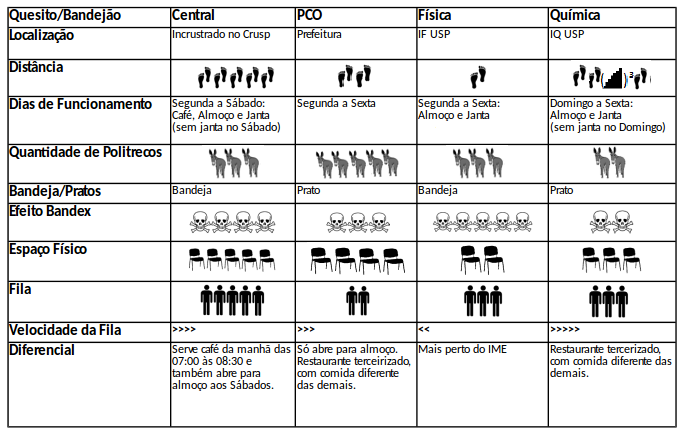
\includegraphics{img/src/bandex.png}
\end{center}
\end{figure}

O horário das refeições ANTES da pandemia da Covid-19 era o seguinte: %REFTIME %PANDEMIA

Café da manhã: 7h às 8h30min (somente no Central, aos sábados fica aberto das
7h às 9h e aos domingos das 8h às 9h30)\\
Almoço: 11h15min às 14h15min (exceto de segunda a sexta na Química, que é das 11h às 14h)\\
Jantar: 17h30 às 19h45 (não tem no PCO)\\

Já o horário das refeições ATUALMENTE, ou seja, período em que vocês bixes 2022 estão 
ingressando, é o seguinte:
Café da manhã: 7h às 8h30min (somente no Central, de segunda a sexta; não sabemos se será
oferecido aos fins de semana)\\
Almoço: 11h15min às 14h15min (em todos os bandejões)\\
Jantar: 17h30 às 19h45 (somente na Química, na Física e no Central)\\

IMPORTANTE: o funcionamento dos bandejões pode ser alterado ao decorrer do ano, por isso
recomendamos que vocês fiquem atentos ao aplicativo e às placas informativas presentes nos
bandejões.

Para mais informações, visitem o site do SAS: {\tt http://sites.usp.br/sas/} ou
utilizem o aplicativo ``Cardápio+ USP''.

\end{subsecao}

\begin{subsecao}{Outros lugares para comer na USP}

Caso vocês, bixes, não queiram comer no bandejão, seja porque estão com medo do
prato do dia ou simplesmente porque querem comer algo diferente (e
possivelmente de sabor melhor), saibam que há alguns outros lugares na USP onde
vocês podem comer; por exemplo, os que estão nesta lista.

%REFTIME
Importante: grande parte das informações a seguir não está tão certa porque já
fazem (pelo menos) três anos que verificamos pela última vez, então sempre que estiver
escrito ``custa R\$ $x$'' interpretem como ``vai custar um tanto a mais que R\$ $x$''.

\textbf{Lanchonete da Física}

Fica um pouco antes do bandejão da Física, nela vocês podem almoçar pagando R\$
40,90 o quilo, sempre tem uma razoável quantidade de saladas e pratos
quentes, além disso, tem churrasco com uma boa variedade de opções.
Além do almoço por quilo, lá vende alguns salgados e lanches como sanduíches e
beirutes. E um pouco antes da lanchonete, há um lugar que vende cookies por R\$
3,50 (3 unidades). Vocês vão sentir o cheiro dos cookies quando forem bandejar.

\textbf{Restaurante do IPEN}

Fica na parte de cima da rua entre o IF e o Parque Esporte Para Todos, para
entrar lá vocês precisam da carteirinha USP. Lá o quilo é R\$ 24,50, porém não
tem uma variedade muito grande de comida, tem marmitex também que é R\$ 11,70.
Ele só abre para pessoas de fora às 13h e antes de ir para o restaurante vocês
devem se identificar.

\textbf{Lanchonete da FAU}

Localizada dentro da FAU assim que você sobe a rampa. Lá além de lanches é
servido almoço tanto por quilo (custa R\$ 43,90) como prato feito. Tirando o por
quilo, qualquer outra coisa deve ser paga no caixa antes de retirar. Além
disso, no terceiro andar da FAU tem a mesinha de doces que os alunos deixam lá
para vender, a variedade e quantidade de doces varia bastante com o dia e o
preço deles costuma ser no máximo R\$2,50.

\textbf{Restaurante da FEA}

Fica atrás da FEA, lá o quilo tem bastante coisa diferente e algumas até que
sofisticadas, porém o preço do quilo lá é R\$61,90, provavelmente é o mais caro
da USP. Geralmente é frequentado por professores e funcionários da USP. Além do
self-service, há algumas opções de prato feito que custam R\$22,00.
\pagebreak

\textbf{Trailers de lanche da \sout{ECA} Química}

Ficam na calçada com a Avenida Lineu Prestes, em frente ao Instituto de
Química. Nesses carrinhos vende pastel, sanduíches, churros, tapioca e salgados
em geral. Os preços dos lanches variam entre R\$3,00 e R\$10,00. As opções de
sanduíches e a quantidade de sabores de tapioca é bem grande e todos em geral
são muito bons. Já o pastel você pode escolher de 1 a 5 ingredientes para pôr
no pastel, portanto o preço varia de acordo com a quantidade de ingredientes que
vocês vão querer.

\textbf{Cachorro-quente da Reitoria}

Fica na rotatória da biblioteca Brasiliana (ou a rotatória depois do CEPE, se assim preferir),
lá o cachorro-quente pode ser feito tanto no pão de cachorro-quente como na baguete. Além disso,
há a opção de pôr catupiry e de pôr uma salsicha adicional. O preço do cachorro-quente varia
entre R\$9,00 e R\$12,00.

\textbf{Poke da Reitoria}

Tem um lugar que vende Poke (um prato havaiano que mistura peixe cru em cubos,
arroz, shoyu e frutas) ao lado do cachorro-quente. Esta iguaria custa
aproximadamente R\$23, e você pode escolher os ingredientes que vão no seu prato,
tipo Spoleto. Dá pra fazer um Poke vegano, com cogumelos em vez de peixe. Além de
Poke, também vende Temakis, Hot Rolls, e até Açaí. A qualidade é boa, mas as filas
podem ser demoradas.

\textbf{Pastel do IEE}

Esse lugar maravilhoso fica a apenas alguns passos do IME. Apenas às terças-feiras,
em um canto escondido do IEE (pergunte a um veterane como chegar!) fica o famoso pastel do IEE.
Há muitas opções de sabores, além de poder comprar um caldo de cana para acompanhar (também tem várias opções de sabores!).

\end{subsecao}

\end{secao}


% Um Pouco Sobre o DCE ---------------------------------------------------------
\begin{secao}{Um Pouco Sobre o DCE}

O Diretório Central dos Estudantes Livre da USP ``Alexandre Vannucchi Leme'' é a
entidade que nos representa: estudantes de todos os campi e cursos da nossa universidade.
Entidade que tem sua história marcada pela defesa da educação pública, liberdade
de organização e atuação política, sobreviveu na clandestinidade por alguns anos
da ditadura militar, por proibição do regime.

No entanto, a ditadura não conseguiu acabar com o movimento estudantil. Contribuiu,
ao contrário, para que os estudantes percebessem seu papel importantíssimo como
protagonistas das mudanças que queriam. A partir dessa união, garantiu-se a
refundação do DCE da USP, em 1976, com caráter LIVRE, que representa a autonomia
dos estudantes e a não vinculação às estruturas do Estado e da reitoria.

No ano de 1973, Alexandre Vannucchi Leme, tinha 22 anos e cursava o quarto ano
de Geologia na USP. ``Minhoca'', como foi apelidado por seus amigos de curso, participava
do movimento estudantil e lutava pela democracia no país. Na manhã do dia 16 de março,
foi levado pelo exército, torturado e morto dois dias depois nos porões do DOI-CODI,
órgão responsável pela perseguição e repressão política na época, em São Paulo.

Em homenagem a ele e a todos os seus semelhantes, vítimas de repressão, o DCE recebe este nome.

Em tempos mais recentes, a necessidade pela defesa da USP pública, gratuita, de qualidade
e democrática se faz cada vez mais necessária e urgente. Para que nós consigamos
garantir essas reivindicações na USP, todos devem ser protagonistas dessa defesa,
por entendermos que é fundamental a existência de uma educação pública com qualidade
em um país marcado pela desigualdade.

Para conhecer melhor o DCE da USP, visite a página no Facebook,
\url{http://www.facebook.com/DCEdaUSP}.

\end{secao}


\quadrinhos{5}

% Hospital Universitário -------------------------------------------------------
\begin{secao}{Hospital Universitário}
   \begin{quote}\emph{O HU USP é o hospital de ensino de excelência utilizado
pelos Cursos de Atenção à Saúde da USP.  O hospital privilegia as pesquisas
relacionadas aos problemas de saúde  mais comuns da população brasileira. O
atendimento é regionalizado para o bairro do Butantã, sempre com enfoque no
ensino e pesquisa''}- trecho obtido da página do HU (\url{http://www.hu.usp.br/})
\textit{alguns} anos atrás.
   \end{quote}

Isso significa que os estudantes de Medicina, Ciências Farmacêuticas,
Odontologia, Saúde Pública, da Escola de Enfermagem e do Instituto de
Psicologia, mantendo contato direto também com os Institutos de Ciências
Biomédicas, de Biologia, de Química, a Faculdade de Arquitetura e Urbanismo,
a Escola Politécnica e a Escola de Comunicações e Artes precisam de cobaias para
suas atividades/experiências. O \sout{USPital} HU é um santo lugar que recebe alguns 
fracos de espírito que bebem demais e ficam incapacitados de fazer qualquer 
atividade fisiológica. Para fazer o cartão do hospital, vocês devem levar:

\begin{itemize}
   \item a carteirinha USP;
   \item um documento oficial com foto (RG, CNH...);
   \item o CPF; e
   \item o CNS (Cartão Nacional de Saúde, do SUS).
\end{itemize}

Assim vocês possuirão alguns privilégios no atendimento, em situações de
emergência vocês são atendidos rapidamente (algo entre 600 minutos, como
diz na senha de espera) e não precisam soletrar o nome da mãe enquanto
estiverem desmaiados.

\begin{description}
\item [Endereço:] Av. Prof. Lineu Prestes, 2565 - Butantã, São Paulo - SP, 05508-000
\item [Telefone:] (11) 3091-9200
\end{description}

\end{secao}


% Tudo Que Vai Volta -----------------------------------------------------------
\begin{secao}{Tudo Que Vai Volta (até bixes)}

\begin{subsecao}{Ônibus}

Se vocês não têm como ir nem como voltar, temos algumas dicas:

\begin{enumerate}
\vspace{-15pt}
  \item Trabalhem muito para comprar um carro,
  trabalhem mais para pagar a gasolina,
  venham para a USP de carro e, obrigatoriamente, deem carona a um veterane;

  \item Peçam a uma pessoa amiga para trazê-los e buscá-los durante seus
  longos anos de IME;

  \item Conheça alguém que, por sorte, mora perto da sua casa, estuda na USP,
  tenha o mesmo horário que você, seja legal e tenha carro. Traduzindo, s-o-n-h-e;

  \item Estiquem o dedão e esperem, esperem, esperem, esperem... a boa vontade
  de alguém para dar carona;

  \item Mudem-se para uma casa perto da USP;

  \item Peguem uma bicicleta e pedalem.

\end{enumerate}
\vspace{-15pt}
OK, vocês decidiram ser bixes normais e pegar ônibus! Nesse caso, vocês
provavelmente estão em uma das seguintes opções:
\vspace{-15pt}
\begin{enumerate}
  \item Vocês vêm de metrô pra USP;
  \item Vocês são super sortudos e acharam um ônibus que vai de casa pra USP.
\end{enumerate}
\vspace{-15pt}
Se vocês vão usar ônibus para ir ou voltar da USP, vocês precisam conhecer
os quatro pontos de ônibus perto do IME: FAU I, Oceanografia, FAU II e FEA.
Até 2019, esses quatro pontos tinham placas com os nomes escritos, mas
agora foram reformados e não têm mais as placas. Mesmo assim, a localização deles
não poderia ser mais intuitiva, veja só:

Tanto o ponto FAU I quanto o ponto da Oceanografia se localizam na Rua do
Matão - FAU I é o ponto que fica mais próximo da FAU, e o da Oceanografia é o
que fica do mesmo lado da calçada que o IO (pronuncia-se i-ó), Instituto de
Oceanografia; os pontos FAU II e FEA ficam na Av. Prof. Luciano Gualberto (que a
partir de agora será chamada de Rua dos Bancos, para todo e todo o sempre),
e, como você já deve estar imaginando, são na frente da FAU e da FEA,
respectivamente. São muitos nomes para lembrar? Fiquem tranquilos: mais
cedo ou mais tarde vocês vão conhecer esses lugares e não vão nem se preocupar
mais com os nomes.


Como você viu ali em cima, nós damos apelidos também intuitivos para as principais
avenidas do campus:
\begin{itemize}
	\item Av. Prof. Luciano Gualberto = Rua dos Bancos;
	\item Av. Prof. Lineu Prestes = Rua do HU;
	\item Av. Prof. Mello Moraes = Rua da Raia.
\end{itemize}

Aqui está a lista de ônibus que passam em cada um dos pontos. Para mais detalhes
sobre cada linha, vocês podem usar o site da SPTrans ou o Google Maps.

\begin{subsubsecao}{Linhas municipais}

{\bf Ponto FAU I}

\begin{center}
	\begin{tabular}{|c|c|c|}
      \hline
	  Letreiro & Cor & Interligações (em ordem)\\
	  \hline
	  8012-10 - Metrô Butantã* & Laranja & Metrô: L4\\
      \hline
	\end{tabular}
\end{center}

{\bf Ponto da Oceanografia}

\begin{center}
	\begin{tabular}{|c|c|c|}
      \hline
	  Letreiro & Cor & Interligações (em ordem)\\
	  \hline
	  8022-10 - Metrô Butantã* & Laranja & Metrô: L4\\
      \hline
	\end{tabular}
\end{center}

{\bf Ponto FAU II}

(Esses os levam pra fora da USP)
\begin{center}
	\begin{tabular}{|c|c|c|}
      \hline
	  Letreiro & Cor & Interligações (em ordem)\\
	  \hline
	  177H-10 - Metrô Santana & Azul & Metrô: L4, L2, L3 e L1\\
	  7181-10 - Term. Princ. Isabel & Laranja & CPTM: L9\\
	  7411-10 - Praça da Sé & Laranja & Metrô: L4, L2, L3 e L1\\
	  7725-10 - Rio Pequeno & Laranja & - \\
	  809U-10 - Metrô Barra Funda & Laranja & L2 \\
	  8022-10 - Metrô Butantã* & Laranja & Metrô: L4\\
      \hline
	\end{tabular}
\end{center}

Esses dois ônibus passam no ponto, mas estão CHEGANDO na USP, preste 
atenção!

\begin{center}
	\begin{tabular}{|c|c|}
	  \hline
	  Letreiro & Cor\\
	  \hline
	  701U-10 - Butantã-USP & Azul\\
	  702U-10 - Butantã-USP & Laranja\\
	  \hline
	\end{tabular}
\end{center}

{\bf Ponto FEA}

(Esses os levam pra fora da USP)
\begin{center}
	\begin{tabular}{|c|c|c|}
      \hline
	  Letreiro & Cor & Interligações (em ordem)\\
	  \hline
	  701U-10 - Metrô Santana & Azul & Metrô: L4, L2, L3 e L1\\
	  702U-10 - Term. Pq. D. Pedro II & Laranja & Metrô: L4, L2 e L3\\
	  7725-10 - Terminal Lapa & Laranja & CPTM: L8\\
	  8012-10 - Metrô Butantã* & Laranja & Metrô: L4\\
	  8032-10 - Metrô Butantã* & Laranja & Metrô: L4\\
      \hline
	\end{tabular}
\end{center}

Novamente, esses quatro ônibus passam no ponto, mas estão CHEGANDO na USP!
\begin{center}
	\begin{tabular}{|c|c|}
	  \hline
	  Letreiro & Cor\\
	  \hline
	  177H-10 - Butantã-USP & Azul\\
	  7181-10 - Cidade Universitária & Laranja\\
	  7411-10 - Cidade Universitária & Laranja\\
	  809U-10 - Cidade Universitária & Laranja\\
	  \hline
	\end{tabular}
\end{center}

As linhas marcadas com um * são as linhas circulares da SPTrans. Segue abaixo suas descrições!

\end{subsubsecao}

\begin{subsubsecao}{Circulares}

Também conhecido como ``circulenda'' ou ``secular'' (aos sábados, ``milenar'',
e aos domingos, ``anos-luz''), é o meio de transporte mais barato dentro da USP.
Foi criado para os USPianos se locomoverem dentro do Campus, mas em muitas vezes
é melhor andar do que ficar esperando. Existem 3 itinerários distintos: 2 deles têm
trajetos aproximadamente reversos e que cobrem todo o Campus, e o outro é uma "versão
expressa" de um deles, que só passa pelas partes do Campus que ficam entre os portões
P1 e P2 (isso inclui o IME, como vocês devem ter visto na tabela do ponto da FEA aí
em cima). Isso já vai ser explicado melhor. Fiquem atentos para não se perderem, hein?

%REFTIME
Em 2021 houve uma grande mudança no trajeto dos circulares, porque agora eles têm um
ponto final no Portão 3 (e tecnicamente não são mais circulares, será que o nome vai ficar?).
Como essa mudança ocorreu durante a pandemia, até mesmo veteranes podem ser surpreendidos,
então prestem atenção nos mapas!

Em 2012 foram implantadas as linhas 8012/10 (circular 1) e 8022/10 (circular 2)
- Metrô Butantã/Cidade Universitária; mais recentemente, em abril de 2019, foi
criada a linha 8032/10 (circular 3), com o mesmo letreiro. Essas linhas funcionam
dentro da USP, e nós alunos não pagamos, pois elas aceitam o bilhete USP
(BUSP - Retire logo o seu!!).

Para acompanharem as rotas dos circulares e acompanhá-los em tempo real, bem como
ver os portões do campus que estão abertos e seu horário de funcionamento, pode-se
usar o aplicativo “Portões USP", disponível para Android e escrito por ex-alunos
do IME.

Para os bixes que não gostam de ler (preferem imagens) colocamos o
mapa das três linhas nas próximas páginas.

\mapa{8012_ida.png}
\mapa{8012_volta.png}
\mapa{8022_ida.png}
\mapa{8022_volta.png}
\mapa{8032_circular.png}

\end{subsubsecao}

\begin{subsubsecao}{Como ir e vir do IME pelo metrô Butantã}

Como sabemos que vocês, bixes, chegam muito perdidos, e muitos pularam todas essas informações
sobre os pontos de ônibus e por isso podem não saber como fazer seu trajeto, resolvemos colocar
aqui um dos trajetos mais comuns que boa parte de vocês vão usar.

Para chegar no IME a partir do metrô Butantã, vocês devem pegar o circular 1 (8012-10) ou o
circular 3 (8032-10). Se vocês pegarem o circular 2 (8022-10), em algum momento vocês vão
chegar no IME, mas os circulares 1 e 3 são muito mais rápidos.

O circular 1 vai fazer o seguinte trajeto: Faculdade de Educação, CEPEUSP, Praça do Relógio
Solar, Biblioteca Brasiliana e Faculdade de Economia, Administração e Contabilidade. A partir
daí, deverão descer no ponto da FEA. O circular 3 faz praticamente o mesmo trajeto até o IME,
sem passar pela Praça do Relógio Solar - isso não significa que você vai sempre demorar
menos para chegar no IME se pegar o circular 3 em vez do 1!

Quando estiverem indo embora, vocês têm duas boas opções: pegar o circular 2 (8022-10) no
ponto da Oceanografia, ou o circular 3 (8032-10) no ponto da FEA. CUIDADO: não peguem o
circular 1 aqui se estiverem querendo ir para o metrô Butantã!!! Lembrem que ele passa na FEA
logo no começo do trajeto (e provavelmente foi nesse ponto que vocês desceram do ônibus quando
chegaram). Se vocês pegarem o circular 1 (8012-10) no ponto FAU I, também vão (em algum
momento) chegar no metrô Butantã, mas boatos dizem que os outros circulares vão mais rápido.
Aí, basta ficar no ônibus sentado (se conseguir um lugar!) até chegar no metrô Butantã, onde
todos do ônibus vão descer.

\end{subsubsecao}

\begin{subsubsecao}{Linhas intermunicipais}

Agora, se vocês moram mais longe ainda (outra cidade, outro estado, outro país,
outra dimensão...) e não querem ou não podem se mudar para São Paulo, existem
algumas linhas de ônibus fretados para cidades mais próximas (ou não). Se a cidade
de vocês não estiver aí, procurem se informar a respeito, pois não significa
necessariamente que não haja ônibus da USP para lá. Aí estão elas:

\begin{itemize}
  \item {\bf Empresa Urubupungá}\\
    Tel: 0800 11 4777
    Site: {\tt www.urubupunga.com.br}\\
    280BI1- São Bernardo do Campo (Centro)\\
    Cor: Cinza\\
    Onde pegar para sair da USP: ponto FAU II\\
    Para mais informações sobre a rota e a tarifa dessa linha, acesse
    \url{http://itinerario.urubupunga.com.br:8080/itinerario/ItinerarioLinha.aspx?lin=46\&emp=1}

  \item {\bf Fretados Jundiaí - USP}\\
    Viação MIMO\\
    Tel: (11) 4606-8222\\
    {\tt www.viacaomimo.com.br}\\
    Principais horários:\\
    Ida: 6h00; 6h30; 7h00; 12h50; 18h00 (na Rodoviária de Jundiaí)\\
    Volta: 11h40; 15h00; 16h40; 17h05; 18h10; 21h00; 22h49 (No ponto FEA)

  \item {\bf ABC}\\
    Osmar: (11) 94710-8604\\
    Marcelo Antonio: (11) 94719-1783

  \item {\bf Santos}\\
    Arca Turismo\\
    (11) 5928-7961\\
    \url{http://www.arcaturismo.com.br}

\end{itemize}

\end{subsubsecao}

\end{subsecao}


\begin{subsecao}{Horário dos Portões: Veículos no Campus}

Saibam por onde entrar na USP. Lembrem-se de terem sempre a carteirinha USP, e-Card
ou comprovante de matrícula com RG em mãos, pois pode ser solicitado principalmente
nos horários de entrada controlada.
\begin{itemize}
  \item {\bf Portaria 1 (P1):} R. Afrânio Peixoto. Funciona 24h por dia todos os
    dias, mas a entrada é controlada para pedestres e carros nos seguintes horários:
    todos os dias das 20h às 5h, aos sábados após as 14h, aos domingos e feriados o
    dia inteiro. É por onde entram os ônibus municipais.

  \item {\bf Portaria 2 (P2):} Av. Escola Politécnica. De segunda a sexta, acesso
  livre das 5h às 20h e controlado das 20h às 0h. Aos sábados, liberada somente para
  pedestres das 5h às 14h e controlada somente para pedestres das 14h às 0h.
  Fechada aos sábados (para veículos), domingos e feriados. Única entrada para caminhões.

  \item {\bf Portaria 3 (P3):} Av. Corifeu de Azevedo Marques. Tem o mesmo horário
    de funcionamento do P1 para os pedestres. Para os carros, tem o mesmo horário do P1
    exceto aos domingos, feriados e madrugadas (0h às 5h), nas quais ele fecha, ao
    contrário do P1.

  \item {\bf Portaria P' (Plinha):} R. Eng. Teixeira Soares. Funciona de segunda a
  sexta das 6h às 18h. Fechado de sábados, domingos e feriados.

  \item {\bf Portarias de pedestre (Mercadinho, São Remo, HU, CPTM e
      Vila Indiana):} Funcionam de segunda a sexta das 5h às 20 h, e de sábado das 5h às 14h.
      Acesso controlado de segunda a sexta das 20h às 0h. Nas portarias do Mercadinho e Vila
      Indiana, pode entrar em quaisquer outros horários, incluindo domingos e feriados, mas o
      acesso é controlado.

\end{itemize}

As linhas de ônibus municipais que passam por dentro da USP não operam aos finais de semana,
com exceção aos circulares, que entram na Universidade a qualquer hora, e à linha 702U (Term.
Pq. D. Pedro II - Cid. Universitária), que funciona todos os dias das 5h às 0h
(aproximadamente!). Se vocês vêm de carro, saibam que a universidade dispõe de bolsões de
estacionamento gratuito em torno das Unidades.

\end{subsecao}
\pagebreak
\begin{subsecao}{Pontos de táxi}
Existem alguns pontos de táxi espalhados pela Cidade Universitária. As frotas
operam de segunda a sexta-feira, das 7h às 23h, além de aos sábados, das 7h às 17h.
Eis suas localidades:

\begin{itemize}
\item Praça das Agências Bancárias\\
Fone: (11) 3091-4488

\item Praça da Reitoria\\
Fone: (11) 3091-3556

\item Hospital Universitário\\
Fone: (11) 3091-3536
\end{itemize}
\end{subsecao}

\end{secao}


% Guia de jogos da Vivência ----------------------------------------------------
\begin{secao}{Guia de jogos da Vivência }

Bixes, como já foi dito muitas vezes, na USP, vocês não devem apenas estudar, mas
também aproveitar TUDO que é oferecido. Se você é alguém que gosta de jogar
baralho, no IME existem muitos veteranes que ficarão felizes em te chamar pra
jogar se estiverem precisando de mais um jogador.

A maior concentração desses veteranes acontece na Vivência, e lá eles jogam
principalmente os seguintes jogos: Truco, Fodinha, Pokeralho, Cagando, Copas, Espadas,
King e Bridge. Como eles sabem que vocês provavelmente nunca ouviram falar desses jogos,
tiveram a bondade de ensiná-los antes mesmo de vocês aparecerem por lá! Aí está um
pequeno manual de jogos de baralho da vivência. Não batam de mico* e
leiam-no com atenção. \footnote{Os termos marcados com um * são explicados no Glossário, no fim do guia de
jogos. Vocês, bixes, provavelmente não vão entender tudo o que está escrito aqui.
Nesse caso, é só ir até a Vivência e pedir, com muita educação, pra qualquer 
veterane que estiver sentado jogando baralho que te ensine o jogo X.}

Vamos então aos jogos!

\begin{subsecao}{Truco}

O Truco é um jogo de boteco, e você já deve ter jogado ou visto alguém jogar em
algum momento da sua vida (não era só você que passava o intervalo da escola ou
do cursinho, e até algumas aulas, jogando Truco...) Ele é jogado por quatro
jogadores formando duas duplas ou 6 jogadores formando 2 trios, que se sentam
alternados à mesa.

Utiliza-se um baralho sem as cartas 8, 9 e 10. No truco a carta mais alta é o 3,
seguido, em ordem, por 2, A, K, J, Q, 7, 6, 5 e 4. 

O carteador (também chamado de 'pé') embaralha o maço e dá ao jogador da
esquerda para que este corte o baralho (por cortar, entende-se dividir o baralho
em duas porções, para que apenas uma delas seja utilizada na distribuição das
cartas). Daí, distribui 3 cartas para cada
jogador e vira uma carta sobre a mesa. Essa carta determina qual será a manilha
do jogo - ou seja, a carta mais forte do jogo. A manilha será sempre a carta
seguinte, em ordem de tamanho, da virada. Por exemplo, se a carta virada for um J,
a manilha será o K. Isso significa que, no jogo atual, o
K passa a ser a carta mais forte. É importante ressaltar que,
entre as manilhas, existe uma hierarquia de naipe. A carta de paus $\clubsuit$ é
a mais forte, seguida da de copas $\heartsuit$, espadas $\spadesuit$ e ouros
$\diamondsuit$.

A pessoa à direita do carteador (também chamada de 'mão') será a primeira a
jogar uma carta. O jogo roda em sentido anti-horário. Todos os participantes
deverão jogar uma carta na mesa seguindo a ordem de jogadores. Aquele que jogar
a carta mais forte ganha a rodada e torna a jogar na próxima rodada. Ganha a
mão a dupla ou trio que fizer duas das três rodadas.

\textit{O truco:}

Na sua vez de jogar, um jogador pode pedir ``TRUCO!!'', aumentando o valor do
jogo para 3 pontos. A parceria adversária pode fugir (e perder apenas um
ponto), jogar valendo 3 pontos, ou pedir ``SEIS MARRECO!'', aumentando mais ainda
o valor do jogo. O valor da rodada pode ser aumentado gradualmente para ``Nove''
ou ``Doze'', sempre oferecendo a oportunidade para a equipe adversária fugir,
perdendo o valor atual da jogada (por exemplo, perdendo seis pontos ao fugir de
um pedido de ``Nove''). 

A rodada melada: Quando a primeira rodada empata, por exemplo, com dois Ases
jogados por duplas diferentes, a rodada é dita 'melada' e a segunda rodada
decide o jogo. Se na segunda rodada ocorrer mais um empate, é a terceira que decide
o jogo. Por fim, se ocorrer mais um empate na terceira rodada, nenhuma equipe leva
o ponto. Por outro lado, caso o empate ocorra apenas na segunda rodada (e não na
primeira), vence a equipe que tiver vencido a primeira rodada. É importante destacar
que, se as duas cartas que empataram a rodada forem manilhas, neste caso em
específico, existe um desempate, que se dá pela força dos naipes. 

A mão de onze: Quando uma das equipes está com 11 pontos, cada jogador dessa
equipe pode checar as cartas do seu parceiro antes de decidir se joga ou não.
No caso de aceitarem o jogo, a rodada vale imediatamente 3 pontos (e não pode
ser trucada, sob pena de perder o jogo). No caso de não aceitarem, a equipe
adversária ganha apenas um ponto. 

A mão de ferro: Quando as duas equipes estiverem com 11 pontos, é chamada
mão de ferro, e será a última mão da partida: aquela que vencê-la
vence o jogo. Esta mão é jogada no escuro, ou seja, nenhum jogador
pode ver as cartas que receber, deve deixá-las na mesa viradas
pra baixo até o momento que jogar a carta. 

O jogo continua assim até que uma das equipes atinja os 12 pontos (ou tentos) e
ganhe a partida.

\end{subsecao}

\begin{subsecao}{Fodinha}

Assim como Truco, Fodinha (Te fode, Se fode aí, entre outras variações de
como é chamado) é um jogo de boteco. Inclusive, Fodinha é o jogo
que você joga quando quer jogar Truco, mas tem uma quantidade ímpar de 
pessoas, pouco baralho para muita gente ou porque não vai dar tempo, entre
outros motivos. Mas, diferentemente do Truco, o Fodinha é um jogo individual,
jogado por 3 ou mais pessoas (o limite máximo é até o que o seu bom senso
permitir de jogadores).

Assim como Truco, também utiliza-se um baralho sem as cartas 8, 9 e 10. A sequência
de cartas é a mesma, sendo que a ordem, da mais forte para a mais fraca, é a seguinte:
3, 2, A, K, J, Q, 7, 6, 5, 4. Além disso, existe uma manilha (se você não sabe o que é,
mais pra frente a gente explica).

A cada mão é distribuído um número diferente de cartas para cada jogador. Os
jogadores começam o jogo com uma carta cada, e a cada mão aumenta em 1 a
quantidade da cartas recebidas até não ser possível mais distribuir essa quantidade de
cartas para os jogadores. A partir daí, o jogo começa a voltar, ou seja, em cada mão uma
carta a menos é distribuída até que uma carta apenas seja distribuída para 
cada um. Essa é a última rodada do jogo.

Após a distribuição, uma carta é virada. Ela determina qual será a 
manilha (mais uma semelhança com Truco) da rodada: dada a carta virada, a manilha será
a que tiver a numeração seguinte (ou seja, caso seja virado um 5, a manilha
será o 6). A manilha será sempre a carta mais mais forte da rodada. Entre as manilhas,
existe uma hierarquia de naipe. A carta de paus $\clubsuit$ é a mais forte, seguida da de
copas $\heartsuit$, espadas $\spadesuit$ e ouros $\diamondsuit$.

Em seguida, rodando no sentido anti-horário e começando pela direita do carteador (quem
distribuiu as cartas), cada jogador deverá "apostar", vendo as cartas que tem em mãos,
quantas rodadas ele acha que pode vencer. Após todos apostarem, começa a 1ª
rodada, na qual cada jogador (na mesma ordem que apostaram) devem descartar uma carta da sua
mão. Quando todos tiverem descartado, o jogador que jogou a maior carta vence a rodada e uma
nova rodada começa, seguindo no mesmo sentido, começando pelo jogador que venceu a última
rodada, até que acabem as cartas nas mãos dos jogadores.

Ao final da mão, cada jogador irá comparar o número de rodadas que fez com o que
apostou e receberá de pontos (ou fodes) o módulo da diferença entre os 2. No final do jogo,
perde aquele que tem mais pontos, e ganha o que tem menos.

Vale ressaltar que, em cada mão, o último jogador a apostar é obrigado a falar um número de
forma que não seja possível todo mundo acertar a aposta, ou seja, se por exemplo está na 7ª rodada
e a soma das apostas dos jogadores até agora é 5, o último jogador não pode apostar que faz 2.

Durante uma rodada, se um jogador joga uma carta de número igual a um que já saiu naquela
rodada, as duas se cancelam e saem da disputa, mesmo que sejam as maiores cartas da rodada,
de forma que uma carta menor faça a rodada. Essa regra não vale para manilhas, pois existe uma
hierarquia entre elas.

A primeira e a última mão são especiais, ou seja, nas duas mãos com apenas uma 
carta, os jogadores colocam a carta que receberem na testa de forma que todos os outros jogadores 
vejam sua carta menos ele próprio. Assim, ele deve fazer sua aposta baseado na cartas dos outros e
não na sua.

\end{subsecao}


\begin{subsecao}{Pokeralho}

Um dos jogos mais jogados da vivência em seu passado, retornando a ser jogado ultimamente, o
Pokeralho é uma mistura de Presidente (também conhecido como milionário) com
Poker. No pokeralho, cada jogador recebe 13 cartas. Quem embaralha e distribui é
selecionado de forma randômica, sendo bixes uma das prioridades quando este sabe
como fazer isso. A ordem das cartas é: 2 A K Q J 10 9 8 7 6 5 4 3, do mais forte
para o mais fraco, exceto nos jogos de Straight, que será explicado mais a
frente. Os naipes também possuem uma ordem, que é: Espadas, Copas, Paus e Ouros,
do mais forte para o mais fraco.

As mãos utilizadas são, em ordem de força e separadas pelo número de cartas:

\begin{itemize}

\item \textbf {1 carta:}
\begin{itemize}
\item Conhecido como \textbf{single}, é uma carta qualquer.
\end{itemize}
\item \textbf {2 cartas:}
\begin{itemize}

\item \textbf{Par:} Quaisquer duas cartas de mesmo valor.
\end{itemize}
\item \textbf {3 cartas:}

\begin{itemize}
\item \textbf{Trinca:} Quaisquer três cartas de mesmo valor.
\end{itemize}
\item \textbf {5 cartas:}

\begin{itemize}
\item \textbf{Straight [Sequência]:} Cinco cartas seguidas, de qualquer naipe,
aqui há uma regra especial, a carta Ás só pode começar ou terminar uma
sequência.
\item \textbf{Flush:} Cinco cartas de um mesmo naipe.
\item \textbf{Full House:} Uma trinca e um par.
\item \textbf{Quadra:} Quatro cartas de mesmo valor, com direito a um descarte
para completar 5 cartas.
\item \textbf{Straight Flush:} Cinco cartas seguidas do mesmo naipe. O Ás só
pode começar ou terminar uma sequência. 
\end{itemize}

\end{itemize}

O jogo se inicia com aquele que tem o $\diamondsuit$3, a carta mais fraca. Ele
então joga uma das mãos acima (não é necessário que ele utilize
o $\diamondsuit$3 nessa jogada, só que ele a tenha), e em ordem, os jogadores
jogam uma mão de mesmo número de cartas e maior força que a anterior ou passam
a vez (ou seja, se alguém abriu uma dupla, as pessoas só podem responder com
uma dupla, se alguém abrir com um jogo de $5$ cartas, então só podem ser
jogadas mãos de $5$ cartas dentre as descritas acima). 

Para os jogos de 1 e 2 cartas, a força é dada primeiro pelo valor da carta e
depois pelo naipe da mesma, assim um $\clubsuit$3  pode ser jogado sobre
um $\diamondsuit$3, mas não sobre $\heartsuit$ 3 ou uma carta de valor 4 ou
maior de qualquer naipe. Para jogos de 3 cartas, a força é dada só pelo valor
da carta. Para jogo de 5 cartas, primeiro vem a força do tipo de
jogada (Straight $<$ Flush $<$ FullHouse $<$ Quadra $<$ Straight Flush). Para duas
jogadas iguais, temos os seguintes critérios:
\begin{itemize}
	\item Straight : a maior carta da sequência é que determina a força.
	\item Flush: o naipe é o primeiro desempate, seguido pela carta de maior
valor.  \footnote{ $\clubsuit$5 $\clubsuit$8 $\clubsuit$9 $\clubsuit$10 $\clubsuit$K é
maior que $\diamondsuit$2 $\diamondsuit$J $\diamondsuit$Q $\diamondsuit$K
$\diamondsuit$A e menor que $\clubsuit$3 $\clubsuit$4 $\clubsuit$6 $\clubsuit$7
$\clubsuit$2 ou qualquer FLUSH de $\heartsuit$  ou $\spadesuit$ }
	\item Full House: é visto pelas cartas da trinca.	
	\item Quadra: valor da quadra. Ignore a carta de descarte.
	\item Straight Flush, quando aparecer um alguém lhe ensina direito.
\end{itemize}

Quando 3 jogadores passarem a vez, o último a jogar torna, podendo escolher
qualquer mão para jogar, inclusive com mais ou menos cartas que a anterior, e o
jogo prossegue assim até que alguém acabe com todas as cartas da sua mão. 

Quando um jogador bate*, as cartas nas mãos dos outros jogadores são contadas e
cada jogador recebe pontos de acordo com o número de cartas que sobrou na mão,
esse número é dobrado se a pessoa tiver entre 7 a 10 cartas, e triplicado se
forem 11 ou mais. Acaba o jogo quando alguém alcançar 51 pontos ou mais, nesse
momento quem tiver menos pontos ganha.

Há uma vertente do pokeralho que é o pokeralho em dupla, onde cada jogador faz
dupla com a pessoa a sua frente, o jogo é procedido normalmente, com algumas
diferenças: 
\begin{itemize}
\item Depois que cada jogador recebe as 13 cartas e as arruma, ele então
escolhe 3 cartas para passar para a dupla, e a dupla escolhe 3 cartas para
passar para o outro jogador (essa escolha deve ser feita sem troca de mensagem
entre os parceiros). 
\item Quando alguém bate, primeiro cada jogador faz a conta do total de pontos
da própria mão (dobrando / triplicando da mesma forma que no pokeralho padrão)
e depois cada dupla soma o total de pontos. 
\item O jogo termina quando uma das duplas faz 102 ou mais, essa dupla perdeu o
jogo. 
\pagebreak
\end{itemize}
\end{subsecao}

\begin{subsecao}{Cagando}

O ``Cagando'', ou ``Cagando no Bequinho'' é um jogo rápido e dinâmico, para ser
jogado em 4 pessoas, que provavelmente vai ser muito jogado nos intervalos das
suas aulas. Como a maioria dos jogos da Vivência, é um jogo de vazas*, onde todos
os jogadores começam com o mesmo número de cartas e jogam uma por vez, no sentido
horário.

Além de ser classificado como um jogo de vazas, o Cagando também testa sua noção
de quão forte está sua mão* e, principalmente, faz você ferrar e rir da
cara dos seus novos amiguinhos bixes.

A cada rodada é distribuído um número diferente de cartas para cada jogador. Os
jogadores começam o jogo com uma carta cada, e a cada rodada aumenta em 1 a
quantidade da cartas recebidas. Na última rodada, cada jogador terá treze cartas.

Depois da distribuição, uma carta é virada e o naipe dessa carta será o trunfo*
da rodada. Rodando para a esquerda a partir do carteador* (sentido horário), cada
jogador chuta o número de vazas que vai ganhar naquela mão (de 0 ao número de
cartas distribuídas).

Para que seja impossível que todos ganhem pontos, o último jogador nunca pode
pedir um número de vazas que faça somar o número de cartas totais. Assim, se 7
cartas foram distribuídas para cada jogador, e as pedidas anteriores foram 3, 0
e 2, o último jogador não pode pedir 2 vazas (completando 7 vazas totais). O
jogo continua, sendo que em cada rodada o primeiro que falou na rodada anterior
será o último a escolher um número de vazas.

Ganha uma vaza a maior carta do naipe da primeira carta, a não ser que um
trunfo seja jogado. O jogador que ganhou a vaza, torna a abrir a próxima vaza. 

No fim da mão, contam-se quantas vazas foram feitas por cada
jogador. Os jogadores que fizeram o número exato de vazas que haviam
dito que iriam fazer, ganham esse número como pontuação. Os jogadores
que erraram perdem o módulo da diferença entre o número de vazas pedidas e feitas
(é, bixes, até na vivência tem matemática; se vocês não sabem o que é isso,
possivelmente um veterane irá te explicar\dots).

Duas rodadas são especiais: a primeira e a última. 

Na primeira rodada, ficaria muito fácil escolher se vocês vão fazer ou não suas
vazas vendo suas cartas, então ninguém pode ver sua própria carta. Em
compensação, vocês podem ver as cartas das outras 3 pessoas, que, assim como
vocês, devem colocar a carta na testa, com a face para os adversários.

Na última rodada, não sobra nenhuma carta para ser virada como trunfo (todas
as 52 cartas foram distribuídas), então a mão é jogada sem trunfo. Além disso,
o carteador dessa rodada é sempre aquele que está em último na pontuação.

\end{subsecao}

\begin{subsecao}{Copas}

Sim, esse jogo é mesmo aquele que você joga no seu computador e sempre acha que
ganha com mais de 100 pontos!! Copas é um jogo muito jogado na vivência e que
vale a pena conhecer.

Copas também é um jogo de vazas, mas aqui todas as mãos são compostas por 13
cartas para cada jogador. Portanto, esse é um jogo a ser jogado por 4 pessoas.

14 das 52 cartas são especiais e valem pontos: cada carta de copas vale 1
ponto, e a dama de espadas (Moça, Mulher, Procurada, Vadia, Pudim...) vale 13
pontos. Portanto, em cada mão são distribuídos 26 pontos.

O jogo termina quando um jogador alcança 100 pontos e o vencedor é aquele que
tem menos pontos.

No começo de cada mão, todos os jogadores devem escolher 3 das suas 13 cartas
recebidas para passar para um adversário previamente determinado. A ordem de
passada é a seguinte: jogador da esquerda, jogador da direita, jogador da
frente e não passar. Ou seja, caso em uma mão as 3 cartas tenham sido passadas
para o jogador da esquerda, na próxima mão elas deverão ser passadas para o
jogador da direita. Por outro lado, caso elas tenham sido passadas ao jogador
à frente, na próxima nenhuma carta deverá ser passada.

Depois da passagem simultânea de todos os jogadores, o jogador com
o $\clubsuit$2 abre o jogo com essa carta.

Em sentido horário, cada jogador, respondendo o naipe*, joga uma carta. Em
outras palavras, um jogador deve respeitar o naipe da vaza caso consiga. Caso
contrário, pode descartar uma carta de outro naipe. O vencedor da vaza é aquele
que jogar a carta de maior valor que respeite o naipe da vaza. Ele recebe todos
os pontos que estiverem na mesma.

Na primeira vaza do jogo, é proibido que os jogadores, se não tiverem nenhuma
carta de paus, joguem uma das 14 cartas de valor do jogo. A partir da segunda
vaza, jogar uma das cartas de valor já é permitido.

Adicionando uma tensão extra ao jogo, um jogador só pode abrir copas (ou seja,
iniciar uma vaza com uma carta de copas) depois que algum outro jogador já
tenha jogado uma carta de copas em uma vaza anterior, de outro naipe.

O jogo prossegue até todas as cartas serem jogadas, contando-se os pontos de
cada um e anotando no placar.

\textbf{Acertando a lua:} Se você conseguir, em uma mesma mão, pegar todos os
pontos em jogo, 26 pontos são adicionados para seus adversários, enquanto você
não ganha nenhum! Se isto levar ao fim do jogo (estourar um jogador com mais
de 100 pontos) e você NÃO FOR GANHAR A PARTIDA, então todos os jogadores
permanecem com seus pontos e você perde 26!

\end{subsecao}

\pagebreak
\begin{subsecao}{Espadas} 

Bixes, se vocês já leram sobre o Cagando, e entenderam meio por cima como é o
jogo de Copas, então Espadas será fácil pra vocês.

Para começar, 13 cartas são distribuídas para cada um dos jogadores, que jogam
em parceria com o jogador à frente. Neste jogo o naipe de espadas será sempre o
trunfo.

Seguindo a partir da esquerda do carteador, cada jogador escolhe o número de
vazas que acha que vai fazer. Como é um jogo de duplas, as pedidas de cada
parceria serão somadas e ambos devem jogar para cumprir esse contrato*. 

Além disso, qualquer jogador pode dizer que não fará nenhuma vaza, um contrato
chamado de NIL, que é especial, pois separa o jogo de seu parceiro, tendo cada
um o seu contrato.

Nesse jogo, um jogador só pode abrir espadas depois que algum outro jogador já
tenha jogado uma carta de espadas em uma vaza de outro naipe.
\begin{description}

\item[Pontuação:]

Para cada vaza de um contrato são atribuídos 10 pontos. Se a parceria falha em
cumprir tal contrato, a dupla perde o valor do contrato. Se a parceria consegue
cumprir tal contrato, ela ganha o valor do contrato, e mais um ponto
na bolsa* da parceria para cada vaza feita a mais que o estipulado.
Se o jogador que fez a vaza tenha pedido Nil, a dupla não ganha mais pontos.
Apenas sobe o valor da bolsa*.

\item[Bolsa:]

Para evitar que os contratos sejam feitos muito baixos, e estimular a precisão
nas escolhas iniciais, cada equipe mantém uma bolsa, que é uma pontuação
separada que vai enchendo conforme vazas a mais que o contrato são feitas. Uma
bolsa estoura quando 10 vazas são adicionadas, tirando 100 pontos da parceria
que fez essas vazas a mais.

\item[O Nil:]
Quando alguém diz que não irá fazer vaza alguma, essa jogada é chamada de Nil.
Tal jogada separa o contrato de seu parceiro, e vale por si só 100 pontos. Um
nil cumprido ganha 100 pontos, enquanto um nil perdido, além de perder tais
pontos, adiciona as vazas feitas na bolsa e não ganha nenhum ponto extra por
vaza.

\item[O Blind Nil:]
Situações dramáticas pedem por atitudes dramáticas, e o Blind Nil é uma delas.
Como o nome já diz, o Blind Nil é pedido sem ver as cartas e por isso, vale o
dobro dos pontos!

\end{description}
Ganha o jogo a equipe que chega em 500 pontos primeiro, ou vocês ainda podem
perder o jogo chegando a -200 pontos. Essa pontuação pode ser alterada pelo
veterane em virtude dos horários de aula ou outros fatores limitantes de
tempo...

\end{subsecao}

\pagebreak
\begin{subsecao}{King}

O King é o jogo mais jogado por nós, IMEanos e também um dos mais mais difíceis.
Originalmente ele é um jogo individual, mas no IME todos nós jogamos em
dupla. É um jogo de vazas e jogado com um baralho de 52 cartas por quatro
pessoas.

O jogo é composto por 10 mãos, 4 positivas e 6 negativas. Em cada uma delas,
cada participante recebe 13 cartas. Cada dupla tem direito a 2 posis e 3 negs.

A cada rodada, um jogador embaralha e distribui as cartas. A pessoas a esquerda
do carteador pedirá posi ou neg* e a pessoa a direita naipe ou tipo. A dupla do
carteador é quem dará a saída do jogo.

Nas mãos positivas do King, o objetivo é fazer o maior número de vazas, e nas
mãos negativas queremos não fazer alguma coisa específica da vaza.

Quando um jogador pede Posi, seu parceiro vai escolher, baseado na própria mão,
um naipe para ser o trunfo. Além dos 4 naipes conhecidos,  os jogadores podem
pedir NT, que é a mão sem trunfo. Geralmente pedimos um naipe em que temos 5
cartas ou mais. Costuma-se pedir NT se o jogador não tiver nenhum naipe longo.

Após a escolha do naipe é jogada essa mão. A dupla que fizer mais vazas ganhará
pontos.

Nas mão negativas do King não existe trunfo e em cada uma delas queremos negar
alguma coisa em específico. As 6 mãos negativas são: Vazas, Copas, Homens,
Mulheres, Duas Últimas (2U) e King.


\begin{list}{\textbf{ (\arabic{qcounter}$^{o}$ mão:)}}{\usecounter{qcounter}}

\item \textbf{Vazas -} O objetivo é fazer o menor número de vazas.

\item \textbf{Copas -}  Nessa neg, deve-se evitar fazer vazas em que tenham
cartas de copas. Nessa mão, os jogadores só podem abrir copas quando só tiverem
cartas de copas na mão.

\item \textbf{Homem -} Nessa mão, deve-se evitar fazer as vazas que tenham Reis
ou Valetes.

\item \textbf{Mulheres -} Nessa mão, deve-se evitar fazer as vazas que tenham
Damas.

\item \textbf{2U -} Nessa neg, deve-se evitar fazer apenas as últimas duas
vazas. Fazer ou não as 11 primeiras não interfere na pontuação.

\item \textbf{King -} Nessa mão, deve-se evitar fazer a vaza que contenha o rei
de copas. Aqui também só é permitido abrir copas quando o jogador só tiver
cartas de copas na mão.

\end{list}

O sistema de pontuação é um pouco complicado. Essa parte pode ser pulada, mas
estará aqui como referência:
\begin{itemize}

\item Vazas:	  20 pontos por vaza
\item Copas:	  20 pontos por carta de copas
\item Homens:	  30 pontos por homem
\item Mulheres: 50 pontos por mulher
\item 2U:	  90 pontos por cada uma das 2 últimas vazas
\item King:    160 pontos pelo $\heartsuit$ K
\item Posi:	  25 pontos por vaza

\end{itemize}

E para aqueles que procuram segredos e leram até aqui: strogonoff

Como jogamos muito mesmo esse jogo, até uma sociedade para jogarmos King foi
criado por alunos daqui do IME. Ela se chama Sociedade Brasileira de King (SBK),
e tem até membros IMEanos já formados. A SBK organiza torneios e variantes do
jogo pra que vocês possam se divertir muito com o seu jogo favorito.

Então, não deixem de aparecer na Vivência e botar em prática todos esses jogos
que vocês acabaram de aprender!

\end{subsecao}

\begin{subsecao}{Bridge}

O Bridge é um jogo pouco conhecido aqui no Brasil mas que é muito jogado em
vários outros países pelo mundo. Usa a mesma dinâmica de vazas dos outros jogos
citados anteriormente e ainda adiciona um contrato* a ser cumprido por uma das
parcerias.

Apesar da sua falta de popularidade no Brasil, uma quantidade significativa de 
veteranes do IME conhecem e jogam o jogo.

O jogo é dividido em duas partes: leilão e carteio. A parte do carteio é bem
parecida com uma Posi no King porém com uma diferença fundamental: as 13 cartas
de um dos jogadores fica à vista, tanto para o seu parceiro quanto para os seus
adversários. Além disso, durante o leilão, várias informações são trocadas entre
as parcerias para tentar se chegar ao melhor número de vazas que podem ser
feitas.

Como já deu pra perceber, o jogo é bastante diferente dos outros e seu
aprendizado é um pouquinho mais complicado, então não vamos explicar nesse Guia
todas as regras, pontuação e convenções utilizadas.

Mas se vocês se interessaram e gostariam de entender o que esse bando de
gente vê nesse jogo, ou o que são aqueles cartões que as pessoas usam antes de
começar a jogar de verdade, não deixem de entrar em contato com os DMs do
Bridge (sim temos Bridge na atlética).

\end{subsecao}

\begin{subsecao}{Glossário:}

Mico: Carta de um naipe que somente um jogador tem.

Bater mico: Jogar um mico. Pode ser uma jogada boa, mas normalmente é
ruim. Ela requer uma percepção de jogo bastante avançada que bixes,
como você, ainda não tem.

Cortar o baralho: Tirar uma quantidade de cartas de cima do baralho para mudar
o ponto onde começa a distribuição das cartas.

Bater: Acabar com suas cartas, terminando, assim, o jogo.

Vaza: Conjunto de 1 carta de cada jogador, jogadas em sentido horário. Todos
devem jogar o mesmo naipe da primeira carta, ou jogar qualquer outra carta se
não tiverem esse naipe.

Mão: Conjunto de (normalmente) 13 cartas que cada jogador recebe várias vezes
durante o jogo. Pode também ser usado como sinônimo de rodada, como
em ``Ganhei 3 pontos na mão anterior''.

Carteador: Aquele que distribui as cartas. Na verdade é mais relacionado com
quem começa jogando (normalmente começa o jogo aquele à esquerda do Carteador),
já que normalmente as cartas são embaralhadas por qualquer um.

Trunfo: Naipe escolhido para ser mais forte que os outros. Em uma vaza, a carta
mais alta do primeiro naipe aberto ganha, a não ser que uma carta com naipe do
trunfo tenha sido jogada. Nesse caso, ganha o trunfo mais alto.

Responder o naipe: Jogar uma carta do mesmo naipe que abriu a vaza, ou jogar
qualquer carta se não tiver uma carta de tal naipe.

Contrato: Número de vazas que uma parceria diz que vai fazer antes das cartas
serem jogadas.

Bolsa: Continua lendo que já chega nessa parte.

Posi(tiva) ou Neg(ativa): Para determinarmos se a mão é boa para jogar Posi ou
Neg usamos uma regrinha em que: o A vale 4 pontos, o K vale 3, o Q vale 2 e o J
vale 1 ponto. A soma de todos os pontos do jogo é igual a 40 que dividido por 4
dá 10 pontos para jogador em média. Assim, se você tem um pouco mais de 10
pontos na mão, é uma boa idéia pedir Posi, e se tiver poucos pontos, é bom
então pedir Neg.

Touchar: É quando um jogador não tem mais cartas do naipe que foi aberto e
descarta uma carta desfavorável aos seus adversários. Por exemplo, em uma Neg
Homens, ele pode jogar um valete em uma vaza que seus adversários estão fazendo.

Cortar:  É quando um jogador não tem mais cartas do naipe que foi aberto e joga
um trunfo.

Baldar: É quando um jogador não tem mais cartas do naipe que foi aberto e
descarta uma carta.

Destrunfar: É abrir uma mão com uma carta do trunfo e fazer com que todos
respondam o naipe com o objetivo de diminuir o número de trunfos dos
adversários.

Void: É quando o jogador vem sem cartas de um determinado naipe ou elas acabam
no decorrer do jogo. “Vim void em paus”. Quer dizer que quando o jogador
recebeu suas 13 cartas, nenhuma delas era do naipe de paus.

Quinto/Quarto/Terceiro: É a distribuição dos naipes em nossa mão. Se temos 3
cartas de copas, por exemplo, dizemos que estamos terceiro em copas. Se tem 1
carta de espadas, dizemos que estamos primeiro em espadas.

Finesse: É uma aposta estatística no posicionamento das cartas para
fazer sua jogada.

\end{subsecao}


\end{secao}


%FIXME GAMBIARRA para não quebrar página num lugar zuado
\pagebreak

% Dicas ------------------------------------------------------------------------
\begin{secao}{Dicas}

Como todos os bixes chegam perdidos, aqui vão algumas dicas pra vocês não
ficarem perguntando o tempo todo:

%TODO Checar isso aqui.
{\bf Bancos e Caixas Eletrônicos:} agências do Santander, Bradesco,
Banco do Brasil, Caixa Econômica e Itaú na Av. Prof. Luciano Gualberto. 

{\bf MatrUSP:} é um site criado por alunos do BCC para simular grades horárias
para matrículas de disciplinas. Assim, vocês conseguem saber direitinho se suas
disciplinas vão coincidir e quanto tempo livre vocês vão ter para ficar na
vivência entre as aulas. Acessem: \url{http://bcc.ime.usp.br/matrusp}

{\bf USPAvalia:} outro site criado por alunos do BCC (pois é, olha só!) que
contém inúmeras avaliações da comunidade sobre disciplinas oferecidas e
seus respectivos professores. Ótimo para saber se vale a pena ou não pegar
essa ou aquela turma de uma dada disciplina, e vocês mesmos podem contribuir com
suas próprias avaliações e comentários! Acessem: \url{https://uspavalia.com}

{\bf Banco de Provas do CAMat:} uma pasta compartilhada com várias provas de
anos anteriores, que é muuuito boa para estudar. Quando estiver chegando aquela
prova daquela matéria difícil, vale a pena dar uma olhada se tem uma prova antiga,
e depois de passar (ou não) também vale colocar a prova que você fez pra ajudar
as próximas turmas! Acessem: \url{https://tinyurl.com/provas-camat}

\begin{subsecao}{Cultura na USP}

Importante lembrar que a entrada em vários desses museus é gratuita para alunos da
USP, então vale muito a pena visitar!

{\bf Museu de Arqueologia e Etnologia (MAE):} ao lado da Prefeitura do Campus,
possui um dos maiores acervos de artefatos arqueológicos e etnográficos do Brasil.

{\bf Museu de Arte Contemporânea (MAC):} próximo ao CRUSP, nele são expostas
produções artísticas nacionais e estrangeiras.

{\bf Museu do Brinquedo:} fica na Faculdade de Educação, Bloco B. Seu acervo conta 
com itens datados do início do século XX, incluindo brinquedos, jogos, materiais
pedagógicos e um acervo fotográfico. Tem a exposição ``Cenas Infantis'', que fica na
biblioteca da Faculdade de Educação.

{\bf Museu do Crime da Polícia Civil:} na Academia de Polícia perto do P1. Seu acervo
reúne ferramentas, objetos e documentos utilizados em delitos de grande repercussão, 
além da história de criminosos cujos atos ficaram marcados na imprensa e na sociedade
brasileira.

% REFTIME
{\bf Museu do Instituto Oceanográfico:} adivinha? Esse museu mantém uma exposição
voltada à dinâmica, à estrutura e à biodiversidade dos oceanos. Até o começo de
2023 ele estava fechado para reformas e sem previsão de abertura.

{\bf Museu da Geociências:} lá mesmo. Conta com amostras de rochas, gemas, meteoritos 
e fósseis. Tecnicamente não faz parte dele, mas o instituto tem um Tiranossauro Rex no
saguão do térreo.

{\bf Instituto Butantan:} próximo à História. É um dos maiores acervos de pesquisa
biológica do mundo, conta com a presença de diversas cobrinhas. % \#VacinaSim \#VacinaJá

{\bf Museu de Anatomia Veterinária:} perto do P3 (portão da Corifeu). Seu acervo
possui uma coleção de dados e fotos de esqueletos, além de modelos anatômicos e
animais preservados.

{\bf Museu de Anatomia Humana:} do lado do HU, seu acervo conta com inúmeras peças
de partes do corpo humano, reais e preservadas, além de modelos anatômicos.

{\bf Orquestra Sinfônica da USP (OSUSP):} faz ensaios abertos no Anfiteatro
Camargo Guarnieri, perto do CRUSP.

{\bf Teatro da USP (TUSP):} fora da USP e próximo do Mackenzie (estação
Higienópolis-Mackenzie), o teatro conta com apresentações frequentes e às vezes
um processo seletivo no final do ano.

{\bf CoralUSP:} realiza apresentações em vários locais de São Paulo, mas geralmente
pode ser encontrado no Anfiteatro Camargo Guarnieri, perto do CRUSP. Ocasionalmente
abrem inscrições.

{\bf Museu Paulista, vulgo Ipiranga:} também fora da USP, no Parque da
Independência - S/N - Ipiranga.

{\bf Museu de Zoologia:} novamente fora da USP, na Av. Nazaré, 481 -
Ipiranga. Sua exposição abriga uma série de animais empalhados, fósseis,
réplica de fósseis etc.

{\bf Museu Histórico da Faculdade de Medicina:} fora da cidade universitária e
dentro da faculdade de medicina da USP, perto da estação Clínicas, o museu contêm
principalmente itens históricos e documentos.

{\bf CinUSP Paulo Emílio:} Dentro do campus, próximo ao bandejão Central,
existe uma sala de cinema. Durante todo o ano ocorrem várias mostras
cinematográficas, nas quais são exibidos inúmeros filmes. As sessões são gratuitas
e a programação pode ser conferida no seguinte site: \url{http://www.usp.br/cinusp/}

\end{subsecao}

\begin{subsecao}{Onde beber?}
	
\quadrinhos{9}
Se vocês são dos bixes que curtem entornar os canecos de vez em quando, então
agora devem estar pensando ``até que enfim vamos falar de algo que presta!'' --
só lembre-se de levar um veterane para pagar a ele algumas doses, pois é graças
a eles que vocês estão recebendo essas dicas. Então sem mais delongas, aqui vão
alguns lugares para se fazer isso à vontade:

{\bf FAU:} na vivência da FAU sempre vende cerveja. Para chegar, basta ir no 
primeiro andar à direita até o fim.

{\bf Física:} embora seja a Física, lá é um lugar gostoso para comer alguns
salgados na lanchonete e tomar algumas cervejas na atlética.

{\bf FFLCH:} vá até o prédio da História e Geografia e vá até o Aquário, fica 
logo à esquerda na entrada do vão, se estiver alguém lá dentro eles vendem cerveja.

{\bf FEA:} entrando na FEA, ande até o final, siga reto depois da biblioteca,
passe por um portãozinho, vire à esquerda e tem uma entrada antes do restaurante.
Lá é a vivência da FEA onde vendem as cervejas geladinhas.

%FIXME Qual é a situação atual do QiB?
{\bf ECA:} famosa Quinta i Breja, adivinha que dia da semana isso acontece?
Acertou, toda quinta-feira na prainha da ECA a partir das 19h!

{\bf Rei das batidas:} muito famoso não só por quem estuda na USP, o Rei,
como é carinhosamente chamado, fica fora da USP, saindo pelo P1. Vende
diversas batidas e, é claro, cerveja. Era mais popular, mas parece que já
perdeu a posição como o \textit{point} de encontro para o Beco (veja abaixo).

% {\bf Bar do frango:} não se sabe qual é o verdadeiro nome desse bar, mas ele é
% uma alternativa ao Rei, quando este se encontra muito lotado. Apesar do péssimo
% atendimento e do aspecto horrível do lugar é bom para beber sem tumulto.
% É frequentado principalmente no começo do ano. Se encontra atrás do Rei.

{\bf Beco da USP:} o famoso ``Beco''. Localizado perto da estação de metrô
Butantã, mais precisamente na Av. Valdemar Ferreira, 55. É um famoso boteco onde
muitos universitários costumam se reunir para descontrair, relaxar e desfrutar de
um menu de cervejas e porções mistas.

É claro que também têm as festas, que ocorrem em qualquer lugar da USP e quase
todas as sextas, e nelas há ainda outras misturas alcoólicas impossíveis. 
No instagram do \url{https://www.instagram.com/rolesdausp/} eles compartilham as 
festas da semana geralmente (mas nem sempre todas).

Por fim, é nosso dever informar que o álcool é uma substância altamente viciante
e, quando bebida em excesso, pode trazer graves consequências à sua saúde, às
vezes à saúde de outra pessoa, à sua família e principalmente ao seu bolso.
Lembrem-se também que é proibida a venda de bebidas alcoólicas dentro da USP,
então não saiam da vivência dos respectivos lugares com a latinha na mão.

\end{subsecao}
\end{secao}


%FIXME GAMBIARRA para não quebrar página num lugar zuado

% Melodias para a bixarada -----------------------------------------------------
%\pagebreak
\begin{secao}{Músicas para a Bixarada}

\begin{subsecao}{Hino Cabeção}
\begin{verse}

Ó IME USP, meu amor\\
Para sempre campeão\\
Cálculo só me traz dor\\
E a REC emoção

Com a cachaça na mão\\
Para teus times vou torcer\\
Jogar com raça e coração\\
Vermelho e branco até morrer

ôôô ôôÔÔ ôôÔÔ ôôÔÔ

Eu vim aqui\\
Só pra gritar\\
Dá-lhe! IME! USP!
\end{verse}
\end{subsecao}

\begin{subsecao}{Musiquinhas de inter}
\begin{verse}

``O IME é o IME do IME"

``IME chupa IME lambe"

``IME ao contrário é M. M de Mackenzie"

``O IME é uma droga, vamos fumar o IME"

``Eu sou do IME, sou mais meu time\\ 
\,Não uso drogas e assisto anime"

\end{verse}
\end{subsecao}
\pagebreak

%\begin{comment}\begin{subsecao}{Caboclo da MAT}

% {\em Cantar como ``Faroeste Caboclo'' da Legião Urbana. Essa música é em memória 
% à FUVEST, quando Matemática Aplicada e POLI pertenciam à mesma carreira}

% \begin{verse}
% \footnotesize{
% Cheio de medo em setembro Joãozinho viu que seus dedos tremiam pra fazer a
% inscrição\\
% Deixou pra trás a namorada, a motoca, o futebol e as festinhas pra rachar na
% revisão\\
% Quando criança só pensava em ser engenheiro ainda mais com o dinheiro que
% sonhava em ter na mão\\
% Era o CDF lá do colégio onde estudava e todo mundo admirava o boletim desse
% cuzão\\
% Ia pra igreja só pra rezar pro seu santo pra pedir a sua ajuda pra prestar
% vestibular\\
% Sabia mesmo que ia ser barra pesada porque tinha muito japa pra tomar o seu
% lugar\\
% O ano todo se propôs a estudar, passava o dia sem ligar a televisão\\
% Nos feriados não ia viajar, ficava em casa treinando redação\\
% Fazia todos os exercícios da apostila e no fim de cada aula ia falar com o
% professor\\
% Às quinze horas ia pro laboratório ver as mitocôndrias da aula anterior\\
% Não entendia como o militarismo dominou nosso país por vinte anos de terror\\
% Ficou cansado de tentar achar resposta e desceu pra lanchonete pra afogar a sua
% dor\\
% E lá chegando foi tomar um cafezinho e encontrou um concorrente com quem foi
% falar\\
% E o concorrente aumentou seu desespero pois manjava muita coisa que ele tinha
% que estudar\\
% Dizia ele, eu vou prestar o ITA... Nesse país prova pior não há\\
% E se não der eu vou pegar engenharia, lá na POLI eu vou tomar o seu lugar\\
% E João não gostou dessa proposta, ele disse ``ai que bosta, eu tô passando mal''\\
% Ele ficou bestificado com a ideia de pegar lista de espera só depois do carnaval\\
% Meu Deus, é pior ainda, no ano novo eu posso estar lá na Mauá\\
% É brincadeira querer ser engenheiro e só descolar emprego em Taguatinga\\
% Na sexta-feira ele morria de vontade de correr pro banheiro se borrando de pavor\\
% E conhecia muita gente arrogante que passava do seu lado se dizendo um terror\\
% Ele estudava o relevo da Bolívia, função quadrática e modular\\
% E nos domingos então ele fazia tarefa mínima e complementar\\
% E Joãozinho até a morte se esforçava e o tempo mal sobrava pr'ele se alimentar\\
% E via às duas horas o Vestibulando que passava todas as dicas sobre o vestibular\\
% Mas ele não queria mais conversa e decidiu que em novembro era hora de rachar\\
% Ele pirou que precisava estudar tanto, virou um bitolado e começou a delirar\\
% E logo, logo os malucos da sua idade viram a calamidade, tem babaca novo aí\\
% E o nosso Joãozinho ficou louco e bateu em todos os japoneses dali\\
% Seus amigos preocupados com a sua sorte deram uma fita de rock pr'ele relaxar\\
% Mas de repente sob uma má influência dos boyzinhos lá do fundo começou a zoar\\
% Já na primeira fase ele penou e só passou porque o corte foi sessenta e três\\
% A demência tomou a sua mente: ``Vocês vão ver, eu vou pegar vocês!!!''\\
% Agora Joãzinho era fodido e estava decidido que não ia se dar mal\\
% Sacava toda a trigonometria e manjava de limites, derivada e integral\\
% Foi quando conheceu uma menina e de toda aquela zona ele se arrependeu\\
% Maria Lúcia era uma bitola linda e o coração dele pra ela o Joãzinho prometeu\\
% Ele dizia que devia estudar, pois engenheiro ele queria ser\\
% Maria Lúcia, pra sempre vou te amar, Engenharia com você quero fazer\\
% O tempo passa e um dia chega a hora de fazer segunda fase coitadinho do João\\
% E ele faz uma prova perigosa diz que espera uma resposta, pode ser um sim ou não\\
% Não vou correndo pra banca de jornal nem pra pátio do cursinho isso eu não faço
% não\\
% Pois eu prefiro ficar na minha casa esperando o resultado com o cu na mão\\
% Maria Lúcia vai comprar o tal jornal e logo após achar seu nome ela procura o de
% João\\
% Mas ela volta com tristeza no olhar, olha pra ele e diz ``você pegou a quarta
% opção''\\
% Você passou na sua quarta opção, você passou na sua quarta opção\\
% Bacharelado em Matemática é um tesão, eu vou sofrer as consequências como um cão\\
% Não é que Joãozinho estava certo, seu futuro era incerto mas foi se matricular\\
% Matriculou-se e no meio da zoeira descobriu que tinha muitos como ele no lugar\\
% Fez inscrição pro remanejamento e talvez no fim do ano transferência ia tentar\\
% E Joãozinho mantinha a esperança de um dia ir pra Poli estudar química\\
% Mas acontece que um tal Professorzzini terrorista de renome apareceu por lá\\
% Ficou sabendo dos planos de Joãozinho e decidiu que com suas notas ele ia se
% ferrar\\
% E ele teve que largar Cálculo 2 mesmo sabendo derivar e integrar\\
% E decidiu deixar Estat pra depois que o Moretin voltasse a lecionar\\
% Professorzzini, professor mais sem vergonha com sua prova enfadonha fez todo
% mundo dançar\\
% Desvirginava bixetes inocentes e o nabo era tão quente que nem dava pra sentar\\
% E Joãozinho há muito não via sua amada, e a saudade começou a apertar\\
% Eu vou pra Poli eu vou ver Maria Lúcia, já está em tempo de a gente se encontrar\\
% Chegando à Poli então ele chorou quando viu Maria Lúcia namorando um japonês\\
% Oh, Maria Lúcia, quanto que você mudou, que estrago que a Poli te fez\\
% Joãozinho era só ódio por dentro e então o japonês para um duelo ele chamou\\
% Amanhã às duas horas no Biênio, ou na Praça do Relógio, seja lá onde for\\
% E você pode escolher as suas armas: derivadas ou matrizes de qualquer versor\\
% Que eu provo que o sub-espaço nulo é o coração dessa piranha a quem jurei o meu
% amor\\
% E Joãozinho não sabia o que fazer quando escutou um papo lá no bandejão\\
% Onde falavam dum duelo que iam ver dizendo a hora, o local e a razão\\
% No sábado então às duas horas toda a Poli sem demora foi lá só pra assistir\\
% Um japa que botava pelas costas, encoxou Maria Lúcia e começou a sorrir\\
% Sentindo um ódio na garganta João olhou pros cabacinhos e pros trouxas a
% aplaudir\\
% E olhou pros pipoqueiros e as bancas de cachorro-quente que passavam por ali\\
% E se lembrou de quando era uma criança e de tudo que vivera até ali\\
% E decidiu entrar de vez naquela dança, se a Poli é um circo, e daí\\
% E nisso o céu abriu seus olhos e então Maria Lúcia ele reconheceu\\
% Ela queria fazer Álgebra 2 pra provar que a Poli não a emburreceu\\
% Politécnico, eu sou homem coisa que você não é, e não me contento em por nas
% costas não\\
% Some daqui filha da puta sem vergonha vai pra casa tocar bronha o seu destino é
% ser bundão\\
% E Joãozinho deu as costas para os dois, foi pra Pura onde encontrou o seu valor\\
% Maria Lúcia se arrependeu depois prestou Fuvest mas no IME não entrou\\
% E a todos declarava que o nosso Joãozinho era gênio que escapou de se foder\\
% Que na alta burguesia lá da Poli todo mundo é bunda mole ninguém sabe o que
% fazer\\
% E foi dar monitoria no cursinho pra avisar aos molequinhos pra não esquecer\\
% Ele queria era avisar toda essa gente engenharia é pra demente que só quer
% sofrer.\\
% }
% \end{verse} \end{comment} 
%\end{subsecao}

\end{secao}


% Utilidades -------------------------------------------------------------------
\begin{secao}{Utilidades}

\begin{subsecao}{Na WEB}

\url{https://usp.br} - Página da USP. Aqui vocês encontrarão notícias e eventos da
universidade, bem como informações gerais.

\url{https://ime.usp.br} - Página do IME. Nesse link, vocês poderão ver detalhes sobre
os cursos e obter informações sobre a faculdade.

\url{https://uspdigital.usp.br/jupiterweb} - Sistema JúpiterWeb. Aqui vocês vão
encontrar a grade horária e, mais tarde, poderão fazer matrícula nas matérias
que irão cursar no semestre. Além disso, podem acompanhar o pagamento de
bolsas e auxílios por ele, e também ter acesso ao seu histórico escolar com
as suas notas.

\url{https://portalservicos.usp.br} ou \url{https://olimpo.usp.br} - Portal com todos os
serviços digitais da USP. Vocês vão reparar que a aba ``Graduação'' na verdade
é o JúpiterWeb disfarçado, então na prática vocês podem só acessar o link acima
que dá na mesma (só é um pouco menos bonito porque é um site mais antigo).

\url{https://edisciplinas.usp.br} - É bixes\dots acham que vai ser essa moleza pra
sempre? Se vocês acham, estão muito enganados! Daqui a pouco vocês vão receber
uma senha para poder enviar seus EPs (vide glossário) nesse endereço\dots
(e não adianta fazerem chantagem emocional que o e-disciplinas só vai aceitar
até 23h59\dots não entendeu? vocês vão entender\dots)

\url{https://facebook.com/SpottedImeUsp} - Viu alguém interessante? Quer mandar uma
cantada pro crush mas tem vergonha? Manda um spotted! Afinal, só o $x$ deve
ficar isolado. Ou achou alguém bacana e com gostos parecidos, que tal mandar um
spotted para fazer novas amizades?

% \url{ www.xkcd.com} - Webcomic sobre matemática e computação. Origem de muitas
% piadas que vocês ouvirão por aí.

E por fim\dots

\url{https://google.com.br} - Tudo o que vocês precisam tá no google. Se não
estiver, então não existe. Aproveitem e procurem o Código de Ética da USP (ou
baixem ele em \url{http://www.prg.usp.br/wp-content/uploads/CodigoEtica.pdf})

\end{subsecao}

\begin{subsecao}{Apps}
	
Alguns dos apps disponíveis na AppStore e PlayStore oferecidos pela própria USP
que podem ajudar. Para ver a lista completa, procure pelo desenvolvedor
``Universidade de São Paulo'' em qualquer uma das duas lojas.

{\bf e-Card USP} - Esse é o app mais importante nesse começo de ano, enquanto
sua carteirinha não chega (ver seção Cartão USP no Júpiter). O aplicativo é uma
carteirinha virtual que te dá acesso a tudo que o cartão físico permite,
inclusive comer no bandejão.

{\bf Cardápio+ USP} - Contém o cardápio dos bandejões e mais outros serviços
da SAS, como creche, saúde mental e moradia. Avisa se o bandejão está fechado
ou com horário reduzido.

{\bf Guia USP} - Mapa dos lugares principais da USP, incluindo os institutos,
restaurantes, bancos e mais. Mostra a localização dos circulares em tempo quase
real, mas não é muito preciso e às vezes trava.

{\bf Campus USP} - Permite acessar a central da Guarda Universitária
diretamente no caso de uma emergência. Contém um mapa com as ocorrências
recentes de segurança.

{\bf Disque Trote USP} - Use esse app para denunciar caso sofra um trote
violento. Se preferir conversar mesmo, também pode ligar para o número de
telefone que está mais embaixo.

\end{subsecao}

\begin{subsecao}{Telefones}

{\bf Disque Trote:} {\tt 0800-012-1090} --
\underline{Não deixe de ligar se você sofrer algum trote violento!!}

{\bf SAS:} Seção de Passe Escolar: {\tt (11) 2648-1863} ou {\tt (11) 2648-1865}

{\bf Serviço de Graduação do IME (mais conhecido como Seção de Alunos:} {\tt (11) 3091-6149}

{\bf Superintendência de Tecnologia da Informação (STI):} {\tt (11) 3091-6400}

%{\bf Plantão de Cálculo e Álgebra Linear (serviço gratuito):} {\tt 3037-1773}
%Diziam que era o orelhão do ime, vai que isso volta, resolvi só comentar^^

\end{subsecao}
\end{secao}


\pagebreak
% Glossário --------------------------------------------------------------------
\begin{secao}{Glossário}

Esta parte é, sem dúvida, uma das mais importantes do guia. Aqui vocês
encontrarão todas as explicações para as maiores dúvidas do universo, apesar de
já sabermos que a resposta para a vida, o universo e tudo mais é 42. Com
certeza, após lerem este trecho sua vida vai mudar: vocês saberão, por exemplo,
porque o céu é azul e com quantos paus se faz uma canoa.

\begin{subsecao}{Sobre as matérias}

{\bf Teorema:} um teorema é uma afirmação que pode ser provada. Provar
teoremas é a principal atividade de quem estuda matemática. Deles surgem Lemas,
Corolários, Proposições, e tantas outras coisas que você só vai entender
completamente o que significam quando precisar escrever sobre eles, o que vai
acontecer logo, logo!

{\bf IC (Iniciação Científica):} grupo de estudantes que se dedicam a um
determinado assunto, sob orientação de alguém da área, paralelamente ao curso.
No caso de estudantes que queiram bolsas de estudo, é adotada uma abordagem
mais rigorosa.

{\bf P1, P2, P3:} \sout{provas} um dos maiores sofrimentos da graduação. 
A intensidade depende de quem ministra a disciplina.

{\bf SUB:} prova que você faz quando vai mal nas P1, P2 e P3, ou quando você
simplesmente não vai. Sua aplicação e utilidade depende de quem é responsável
pela matéria.

{\bf REC:} prova que você faz quando vai mal na SUB. Para fazer a REC, precisa
ter pelo menos média 3 nas outras avaliações.

{\bf DP:} matéria que você faz quando vai mal na REC.
\end{subsecao}

\begin{subsecao}{Sobre programas}

{\bf Computador:} objeto com vontade própria, sensível, que requer muito
carinho e atenção.

{\bf EP:} Exercício-Programa. Algo que você vai ter que fazer muitas vezes, e
vai dar muito trabalho.

{\bf GCC:} compilador mais recomendado para seus EP's, por suas inúmeras
qualidades. Atenção: ele ainda fará você se sentir incompetente.

{\bf Hello World:} um clássico da programação universal.

{\bf Segmentation Fault:} efeito computacional aleatório causado pela ``véspera
de entrega de EP''. Desenvolvido por Murphy.

{\bf Stack Overflow:} mensagem que aparece na tela do computador
quando ele se recusa a funcionar. Também é um site com todas as respostas
para todas as perguntas sobre programação: \url{https://stackoverflow.com/}.

{\bf Teorema Fundamental do EP:} ``O EP só funcionará no dia da entrega.'' Não
confunda com o Corolário 42 da Lei de Murphy: ``O EP só {\bf não} funcionará no
dia da entrega!''

{\bf Linux:} sistema operacional criado totalmente em linguagem C, graças a um
esforço mundial de milhares de experts em programação e informática, composto
por aproximadamente 7 mil arquivos e 5 milhões de linhas, e com o qual você não
tem capacidade para trabalhar.

{\bf Windows:} Vírus. Porém tão bem mascarado que parece até a coisa correta a
se usar.
\end{subsecao}

\begin{subsecao}{Sobre a USP}

{\bf CEPE:} Centro de Práticas Esportivas - lugar onde você poderá praticar
todos os esportes que quiser.

{\bf SAS:} Superintendência de Assistência Social. É onde estudantes fazem as
carteirinhas de passe de ônibus, EMTU e metrô, além de solicitar os auxílios
eteceteras que estão explicados na respectiva seção.

{\bf CRUSP:} Conjunto Residencial da USP. Se você se inscrever, torça para
pegar um apartamento num dos blocos já reformados, ou então torça para não
conseguir nenhum.

% {\bf Colmeia:} conjunto de favos.

% {\bf Favos:} um monte de prédios hexagonais encravados no meio do CRUSP.

{\bf CINUSP:} Cinema da USP, localizado no favo 4 da Colmeia. Toda semana ele
passa um filme de qualidade. Informe-se sobre a programação em
\url{https://www.usp.br/cinusp}.

{\bf Pelletron:} prédio da Física que na realidade é um acelerador de
partículas.

{\bf P1, P2, P3:} não confundir com as do item das matérias. Aquelas eram
{\bf as} P1, P2, P3; estes aqui são {\bf os} P1, P2, P3. São os portões da USP.
O P1, que é o principal, se localiza no cruzamento da Av. Afrânio Peixoto com a
Rua Alvarenga, além de ser por ele que entram os circulares vindos do metrô.
O P2 fica na Av. Escola Politécnica. Já o P3 fica na Av. Corifeu de Azevedo
Marques. Fique atento quanto aos horários dos portões, pois eles não ficam
abertos o tempo todo.

{\bf H.U. (Hospital Universitário):} para onde são mandades bixes que se
machucam na Semana de Recepção. Lá são realizados os tratamentos e experiências
com exposição à radiação, exposição a aspirantes a médicos, teste de
paciência/resistência a dor assim que pega a senha, alto nível de gesso no
estômago, queda espontânea (ou não) de cabelo etc.

{\bf Vet (Veterinária):} para onde são mandades biches que se machucaram na
Semana de Recepção.

{\bf Psico:} para onde são mandades bixes (e veteranes também) que querem
plantões psicológicos, porque saúde mental é importante e deve ser tratada com
seriedade. Ponto.

\end{subsecao}
\end{secao}


\pagebreak
% Considerações Finais ---------------------------------------------------------
\begin{secao}{Considerações Finais}

Este guia chegou ao fim. Vocês devem estar pensando ``E agora? O que nós, bixes,
vamos fazer, sozinhes nessa faculdade?''.

Se precisarem de alguma ajuda, basta procurarem alguém que entrou anteriormente
na USP, que essa pessoa te ajudará (provavelmente ela também não saberá a 
resposta, mas talvez conheça alguém que saiba).

Não esqueçam de comprar o kit-bixe para ajudar a Comissão e tornar a recepção
do ano que vem tão legal quanto a de vocês. Participem da Semana de Recepção,
carinhosamente preparada pelo Instituto e por veteranes devidamente
identificades. Último conselho: guardem este guia para o resto de sua graduação.
Por mais ``veteranes'' que sejam, vocês precisarão dele.

Sugestões, elogios, presentes, bajulações ou quaisquer outras coisas para a
Comissão podem ser enviadas para: \url{https://www.facebook.com/recepcaoimeusp} 
ou para o nosso instagram @imeusp.recepcao

Se encontraram algum dos vários erros espalhados como exercício pelo texto,
nos enviem uma mensagem, ou \textbf{participem da Comissão de Recepção 
no ano que vem} e ajudem vocês também na próxima edição do Guia de Bixe!

\end{secao}


%FIXME
%REFTIME
% O guia precisa ter um número de páginas totais múltiplo de 4, e a última
% página tem que estar vazia


\end{document}
